\documentclass[conference]{IEEEtran}
\IEEEoverridecommandlockouts
% DAS732 A2 report - Team Silica. Build: python build_report_assets.py && latexmk -pdf main.tex
\usepackage[utf8]{inputenc}
\DeclareUnicodeCharacter{221D}{\ensuremath{\propto}}
\DeclareUnicodeCharacter{2074}{\textsuperscript{4}}
\usepackage{cite}
\usepackage{amsmath,amssymb}
\usepackage{graphicx}
\usepackage[caption=false,font=footnotesize]{subfig}
\usepackage{booktabs}
\usepackage{algorithm}
\usepackage{algorithmic}
\usepackage{listings}
\usepackage{xcolor}
% siunitx clashes with the local MiKTeX kernel; minimal replacements:
\newcommand{\celsius}{\ensuremath{^\circ}C}
\newcommand{\degree}{\ensuremath{^\circ}}
\newcommand{\si}[1]{#1}
\usepackage{url}
\usepackage{array}
\usepackage{adjustbox}
\usepackage[hidelinks]{hyperref}
\graphicspath{{../images/}}

% float handling: many full-width figures
\extrafloats{250}
\renewcommand{\topfraction}{0.95}
\renewcommand{\dbltopfraction}{0.95}
\renewcommand{\bottomfraction}{0.6}
\renewcommand{\textfraction}{0.05}
\renewcommand{\floatpagefraction}{0.75}
\renewcommand{\dblfloatpagefraction}{0.75}
\setcounter{topnumber}{4}
\setcounter{dbltopnumber}{4}
\setcounter{totalnumber}{6}

\lstset{basicstyle=\ttfamily\scriptsize, breaklines=true, frame=single, columns=fullflexible,
        keywordstyle=\color{blue!60!black}, commentstyle=\color{green!40!black}, showstringspaces=false,
        numbers=left, numberstyle=\tiny\color{gray}, xleftmargin=1.5em}

\newcommand{\figfull}[3]{\begin{figure*}[!t]\centering\includegraphics[width=\textwidth]{#1}\caption{#2}\label{#3}\end{figure*}}
\newcommand{\figfullw}[4]{\begin{figure*}[!t]\centering\includegraphics[width=#4\textwidth]{#1}\caption{#2}\label{#3}\end{figure*}}
% file paths: robust in captions and tables (\path is not allowed in moving arguments); breakable after / and _
\makeatletter
\def\fpath@brk#1{\ifx#1\@nil\else\ifx#1/\string/\allowbreak\else\ifx#1_\string_\allowbreak\else\string#1\fi\fi\expandafter\fpath@brk\fi}
\DeclareRobustCommand{\fpath}[1]{\texttt{\expandafter\fpath@brk\detokenize{#1}\@nil}}
\makeatother
\newcommand{\Tmax}{T_{\max}}
\newcommand{\degC}{\si{\celsius}}

\begin{document}

\title{Scientific and Information Visualization of gridMET Weather (July--September 2024) and Reddit Top Posts\\[0.2em]
{\large DAS732 Data Visualization, Assignment~2 --- Team Silica}}

\author{\IEEEauthorblockN{Sidhanth Prabhu}
\IEEEauthorblockA{BT2024027\\IIIT Bangalore\\Bengaluru, India}
\and
\IEEEauthorblockN{Shrey Modi}
\IEEEauthorblockA{BT2024125\\IIIT Bangalore\\Bengaluru, India}
\and
\IEEEauthorblockN{Parthsarati Samanta}
\IEEEauthorblockA{BT2024083\\IIIT Bangalore\\Bengaluru, India}}

\maketitle

\begin{abstract}
We apply six visualization techniques to two datasets. The scientific-visualization (SciVis) part uses daily 4\,km gridMET fields over the
contiguous United States (CONUS) for 1~July--30~September~2024. We sample eight dates with a documented hybrid rule
anchored on events that we verified in the data: the July western heat wave and Hurricanes Beryl, Debby, Francine and
Helene. On these dates we study (S1) colour mapping of maximum temperature and precipitation: continuous vs.\ rainbow,
discrete, logarithmic and diverging maps, and global vs.\ local normalisation. We study (S2) contour mapping of vapour pressure
deficit with our own vectorised Marching Squares implementation. It resolves saddles with the asymptotic decider and matches
\texttt{scikit-image} segment for segment (21,715 of 21,715 segments). We also compare it with filled contours. Finally we study
(S3) quiver plots and streamlines of the 10\,m wind, covering grid sampling, aliasing, proportional vs.\ uniform arrows and three
streamline seeding strategies. The information-visualization (InfoVis) part derives four new structures from our A1 dataset of
49,266 all-time top posts of 50 subreddits. (I1) A 671-node bipartite subreddit--domain network is drawn with five
layouts and compared on runtime, edge crossings and community separation, with filtering and an interactive version. (I2)
D3.js parallel coordinates with cluster-based edge bundling, brushing and axis reordering, and a zoomable treemap with three
hierarchy remodels and five tiling strategies. (I3) Hand-built horizon plots and ridgeline plots at several groupings and
granularities. Every figure comes with data-grounded inferences, and a cross-task discussion relates heat, moisture and wind on
the same dates.
\end{abstract}

\begin{IEEEkeywords}
scientific visualization, colour mapping, marching squares, quiver plot, streamlines, gridMET, network layout, parallel
coordinates, edge bundling, treemap, horizon graph, ridgeline plot
\end{IEEEkeywords}

% ============================================================================================
\section{Introduction}
\label{sec:intro}
Assignment~2 asks each team to practise scientific visualization (SciVis) on a gridded geophysical dataset and
information visualization (InfoVis) on the tabular dataset it used in Assignment~1 (A1). There are three tasks per
domain. Each member owns exactly one SciVis and one InfoVis task, with no joint ownership apart from the shared data
preparation (Table~\ref{tab:contrib}).

\textbf{SciVis.} We use gridMET~\cite{abatzoglou2013,gridmet_site} for the three-month slice 1~July--30~September 2024
(92 days). % TODO verify: slice confirmed via the TA Google form
Late summer 2024 was meteorologically rich over CONUS. Four landfalling Atlantic hurricanes (Beryl, Debby, Francine and
Helene~\cite{nhc_tcr}) and a long western heat wave give spatially sharp, physically interpretable structure in all
three quantities we visualize: temperature (S1), atmospheric dryness (S2) and wind (S3). A quiet summer would be dominated
by smooth climatological gradients. These events instead put local extremes next to large-scale patterns, which is
exactly what tests colour normalisation, contour placement and vector sampling.

\textbf{InfoVis.} Our A1 dataset holds the roughly 1,000 all-time top posts of each of 50 large subreddits, 49,266 posts in
total, posted 2011--2024~\cite{kaggle_reddit}. Each post has a score (net upvotes), upvote ratio, comment and crosspost
counts, a timestamp, a post type and a link domain. None of the required structures (a network, hierarchies, a
multivariate table and time series) exists as such in the data. Section~\ref{sec:data} documents how each was derived.

\textbf{Tooling.} The work uses Python with xarray~\cite{hoyer2017}, Matplotlib~\cite{hunter2007}, Cartopy~\cite{cartopy},
scikit-image~\cite{vanderwalt2014} and NetworkX~\cite{hagberg2008}, plus D3.js v7~\cite{bostock2011} for the
browser views and Playwright~\cite{playwright} for scripted high-resolution screenshots. Every figure regenerates with one
command per task (README). Figures are numbered as in \fpath{images/}, and the figure index is
Table~\ref{tab:figindex} in the appendix.

\begin{table}[!t]
\centering
\caption{Contribution table. Each member owns one SciVis and one InfoVis task; only data preparation is shared.}
\label{tab:contrib}
\footnotesize
\begin{tabular}{p{1.9cm}p{2.9cm}p{2.8cm}}
\toprule
Member & Owned tasks & Shared data-preparation part \\
\midrule
Sidhanth Prabhu (BT2024027) & S1 colour mapping (+ GIFs); I1 node-link diagram, layouts, filtering, GEXF/PyVis & gridMET download, schema inspection, subsetting and unit conversion \\
Shrey Modi (BT2024125) & S2 Marching Squares, filled contours (+ GIF); I3 horizon and ridgeline plots & A1 cleaning; network, hierarchy, multivariate and time-series derivations \\
Parthsarati Samanta (BT2024083) & S3 quiver and streamlines (+ GIF); I2 D3 parallel coordinates and zoomable treemap & Wind decomposition, statistics tables and evidence-based date selection \\
\bottomrule
\end{tabular}
\end{table}
% TODO verify: split of the shared preprocessing between members (assigned by us; edit if different)

\subsection{The gridMET dataset}
gridMET combines the spatial detail of PRISM climatologies with the daily temporal attributes of the North American Land
Data Assimilation System (NLDAS-2)~\cite{mitchell2004nldas} to give daily surface meteorology on a
$1/24^\circ$ (about 4\,km) grid~\cite{abatzoglou2013}. Our files cover 25.07--49.40\,$^\circ$N and 124.77--67.06\,$^\circ$W
with $585\times1386$ cells, of which 483,879 (59.7\,\%) are land cells inside the CONUS mask. Wind speed and direction in gridMET
come from NLDAS-2 at about 1/8$^\circ$ and are interpolated to the 4\,km grid,
so wind is smoother than temperature or precipitation. Every value is a \emph{daily} aggregate: a daily mean
for wind and VPD, a daily maximum for temperature and humidity, and a daily total for precipitation. The global attributes state that a gridMET day
ends at midnight MST (07~UTC of the next calendar day). This matters for timing a hurricane landfall
(Sec.~\ref{sec:dates}).

\subsection{Choice of the eight time instances}
\label{sec:dates}
The assignment allows uniform or random sampling of 5--10 instances. We use a \emph{hybrid} rule so that the dates are
both spread over the season and centred on interpretable events. Each candidate event was first checked in the
data, not assumed. For every day we computed (Fig.~\ref{fig:01}, \fpath{daily_evidence.csv}):
\begin{itemize}
\item the CONUS maximum of $\Tmax$, and the share of western-US land (31--49.4\,$^\circ$N, 124.8--104\,$^\circ$W) with
  $\Tmax\ge40$\,\degC;
\item the area-mean precipitation and the maximum daily-mean wind in four landfall boxes. The boxes are TX coast
  (27--32\,$^\circ$N, 97.8--93.5\,$^\circ$W), FL--GA--SC (26--34\,$^\circ$N, 84--78.5\,$^\circ$W), Louisiana
  (28.8--33\,$^\circ$N, 93.8--88.5\,$^\circ$W) and Southeast (29--37\,$^\circ$N, 86--80\,$^\circ$W);
\item the CONUS maximum and 99th percentile of wind speed.
\end{itemize}
The rule takes \textbf{six event anchors}, each the seasonal maximum of its indicator. To these it adds \textbf{two
fillers} that split the only long event-free gap (5~Aug--11~Sep, 37 days) into thirds. Consecutive dates are therefore
12--16 days apart, close to uniform sampling (92/8 = 11.5 days). The one exception is the deliberate Helene
landfall/inland pair, which lets S3 show the storm moving. Table~\ref{tab:dates} lists the dates and their evidence. All
three SciVis tasks use the same dates (D1--D8) so that results can be compared across tasks.

\figfull{Fig_01_date_selection_timeline.png}{Daily evidence used to choose the eight analysis dates (vertical lines,
labelled D1--D8), gridMET 1~Jul--30~Sep 2024. (a) Hottest CONUS cell (solid) and share of western land with
$\Tmax\ge40$\,\degC{} (dashed). (b) Area-mean daily precipitation in four landfall boxes. (c) Maximum daily-mean 10\,m wind
in the same boxes. (d) CONUS maximum and 99th percentile of daily-mean wind.}{fig:01}

\input{generated/tab_dates}

\textbf{Inferences from Fig.~\ref{fig:01}.}
(i) The heat wave is the dominant July signal. The hottest CONUS cell stays above 52.5\,\degC{} from 4 to 12~July and peaks at
53.85\,\degC{} on 6~July at 36.48\,$^\circ$N, 116.89\,$^\circ$W (Death Valley). The western area above 40\,\degC{} peaks
twice, at about 12--13\,\% around 6--11~July and at 13.6\,\% on 24~July (D2), so D2 is the date with the most
\emph{widespread} heat, not the hottest single cell.
(ii) Each hurricane box has exactly one dominant rain spike, and it matches the landfall date: Texas 40.0\,mm on 8~July (Beryl),
FL--GA--SC 60.1\,mm on 5~August (Debby), Louisiana 54.4\,mm on 11~September (Francine) and the Southeast 93.5\,mm on
26~September (Helene). Helene's area-mean rain is 1.6 times Debby's and covers the largest box. This matches its reported
catastrophic inland rainfall~\cite{nhc_tcr}.
(iii) Daily averaging damps hurricane winds strongly. The highest daily-mean wind of the whole season (16.1\,m/s) occurs
both on 26~September in Florida (Helene) and on 18~September over Wyoming (42.69\,$^\circ$N, 106.06\,$^\circ$W, a
non-tropical mountain-wind event). Only Helene lifts the CONUS 99th percentile above 10\,m/s. Hurricane winds in gridMET
are therefore an order of magnitude below reported peak gusts; we interpret the S3 wind fields as storm-scale circulation,
not as damaging-wind maps.
(iv) Late September is clearly cooler. The CONUS maximum stays at or below 42.6\,\degC{} from 12 to 22~September (minimum 38.2\,\degC{} on 16~September) and the western area
$\ge40$\,\degC{} drops to 0\,\%, so the season moves from heat-dominated in July to storm-dominated in September. This
contrast drives the global-vs-local normalisation discussion in S1.
(v) Day boundaries matter. Helene made landfall as a Category~4 hurricane about 10~miles west-southwest of Perry,
Florida, at 03:10~UTC on 27~September (11:10~pm EDT on the 26th)~\cite{nhc_tcr},
which falls inside gridMET day 26~September. That is why D7 has the landfall rain and wind maximum while D8 shows the inland
decay.

\subsection{The A1 dataset}
The A1 table merges 50 CSVs (871--1,000 posts each) with 19 columns. A1 established, and we re-checked, several facts.
There are no duplicate ids. Timestamps use two formats (48,279 ISO, 987 \texttt{M/D/YYYY H:MM} in AskReddit). Coverage
is strongly skewed in time: 2011--2015 contribute only 778 posts, while 2020 alone contributes 11,493, because the
corpus is the all-time top tail and recent years have had less time to accumulate votes. Five columns are uninformative
or almost empty and are dropped (Sec.~\ref{sec:a1clean}).

% ============================================================================================
\section{Data Handling and Preprocessing}
\label{sec:data}
Every decision below is also logged, with counts, in \fpath{notes/preprocessing_log.md} (reproduced in
Appendix~\ref{app:log}).

\subsection{gridMET download and inspection}
\textbf{Download.} \fpath{download_gridmet.py} fetches \texttt{vs, th, tmmx, pr, vpd, rmax, srad} for 2024
(28--205\,MB each, about 820\,MB in total) from the repository listing, which we verified rather than assumed. It shows
a progress bar and resumes partial downloads with HTTP \texttt{Range} requests; one interrupted download was resumed
successfully. Because the files are small, server-side OPeNDAP subsetting was not needed.

\textbf{Raw schema.} \fpath{inspect_raw.py} prints each file without CF decoding, so we see what is on disk.
Every variable is stored as \texttt{uint16} with \texttt{\_FillValue}=32767, under a long CF name that differs from the
file abbreviation. The names are \texttt{air\_temperature}, \texttt{precipitation\_amount}, \texttt{wind\_speed},
\texttt{wind\_from\_direction}, \texttt{mean\_vapor\_pressure\_deficit}, \texttt{relative\_humidity} and
\texttt{surface\_downwelling\_shortwave\_flux\_in\_air}. The packing is variable-specific:
temperature uses \texttt{scale\_factor}=0.1 and \texttt{add\_offset}=220\,K; VPD uses 0.01; direction uses 1.0; the
others use 0.1. Dimensions are \texttt{(day, lat, lon)} = (366, 585, 1386), \texttt{day} is ``days since 1900-01-01'',
and \textbf{latitude is stored in descending order} (49.40\,$\rightarrow$\,25.07\,$^\circ$N).

\subsection{Subsetting, masking and unit conversion}
\textbf{Lazy loading.} Files are opened with dask chunks equal to the on-disk chunking $(61, 98, 231)$, and one variable
is processed at a time, so the full year (594\,MB per variable when decoded) is never in memory at once.

\textbf{Temporal subset.} 1~Jul--30~Sep~2024 gives 92 days. \texttt{day} is renamed \texttt{time}.

\textbf{Orientation.} We \emph{sort latitude ascending} once during preprocessing. Every downstream routine then uses
the same convention: image origin at the bottom, \texttt{streamplot} requiring increasing $y$, and Marching-Squares row
0 being the southern edge. This removes a whole class of flipped-map errors.

\textbf{Masking.} CF decoding applies the scale and offset and turns the fill value into NaN. The land mask is
\emph{identical} for all seven variables and constant across all 92 days: 483,879 of 810,810 cells, checked cell by cell.
NaN cells (ocean, Canada, Mexico) are never interpolated. Plots show them in a neutral blue-grey labelled ``No data''.

\textbf{Units.} Temperature is converted with
\begin{equation}
T[\si{\celsius}] = 0.1\,n + 220 - 273.15,
\end{equation}
where $n$ is the stored integer. Precipitation stays in mm\,day$^{-1}$, wind in m\,s$^{-1}$, VPD in kPa, $r_{\max}$ in \%
and $s_{rad}$ in W\,m$^{-2}$. Outputs are float32 NetCDF with zlib compression
(\fpath{data/processed/gridmet_<var>_2024JAS.nc}).

\textbf{Plausibility of extremes.} No values were clipped, because all extremes have a physical explanation. The maximum
$\Tmax$ is 53.85\,\degC{} (6~Jul, Death Valley). The \emph{minimum} daily maximum is $-6.35$\,\degC{} (23~Aug,
41.40\,$^\circ$N 122.18\,$^\circ$W), which is the summit of Mt~Shasta at about 4,300\,m, so the 4\,km grid resolves
high-elevation cold spots. The largest daily rain total is 401.4\,mm (4~Aug, 27.40\,$^\circ$N 82.39\,$^\circ$W, Sarasota--Manatee
coast) in Debby's rain band.

\subsection{Wind decomposition}
gridMET stores the \emph{meteorological} direction $\theta$: where the wind blows \emph{from}, in degrees clockwise from
north. Quiver plots and streamlines need the vector the air moves \emph{toward}, so
\begin{equation}
u = -v_s\sin\theta,\qquad v = -v_s\cos\theta \qquad(\theta\ \text{in radians}).
\label{eq:wind}
\end{equation}
The built-in sanity check gives the following. A westerly ($\theta=270^\circ$) at 10\,m/s gives $u=+10$, $v=0$ (air
moving east). A northerly ($\theta=0^\circ$) gives $v=-10$. $\theta=90^\circ$ gives $u=-10$, and $\theta=180^\circ$ gives
$v=+10$. Values $\theta=0$ (63,867 cell-days) and $\theta=360$ (42,580) are equivalent and decompose identically. Only 39
cell-days have $v_s<0.5$\,m/s, so undefined calm-wind directions are negligible. Over Florida on D7 this gives
$(u,v)\approx(-6,+11)$\,m/s at Tampa from $\theta=151^\circ$, $v_s=12.5$\,m/s. That is a south-south-easterly wind blowing
toward the north-north-west, consistent with Helene's counter-clockwise circulation east of its centre. The u/v fields are
stored in \fpath{gridmet_wind_2024JAS.nc}. Cartopy then rotates the geographic east/north components into the Lambert
conformal map frame.

\subsection{Statistics and derived fields}
For every variable and day we store $n$, min, max, mean, standard deviation and the 1st/5th/25th/50th/75th/95th/99th
percentiles (\fpath{stats_per_day.csv}), plus the same over the whole period (Table~\ref{tab:global}).
Table~\ref{tab:perdate} lists the values on the eight dates. The anomaly used for diverging maps is
\begin{equation}
a_{ij}(t) = \Tmax{}_{ij}(t) - \frac{1}{92}\sum_{t'}\Tmax{}_{ij}(t'),
\label{eq:anom}
\end{equation}
so it is relative to each cell's own Jul--Sep 2024 mean. This removes the elevation and latitude signal and leaves only
weather.

\input{generated/tab_global}
\input{generated/tab_perdate}

\textbf{Normalisation formulas used in S1--S3.} A colour map $C:[0,1]\rightarrow\mathrm{RGB}$ is applied to a normalised
value $\hat{x}$. We use linear normalisation $\hat{x}=(x-x_{\min})/(x_{\max}-x_{\min})$ with either \emph{global} bounds
(over all 92 days) or \emph{local} bounds (the current day). Logarithmic normalisation is
$\hat{x}=(\log x-\log x_0)/(\log x_1-\log x_0)$ with $x_0=0.1$\,mm, applied only to $x>0$. The two-slope diverging
normalisation maps $[x_{\min},0]\rightarrow[0,0.5]$ and $[0,x_{\max}]\rightarrow[0.5,1]$, so zero always sits at the
neutral centre colour. Discrete classes use a \texttt{BoundaryNorm} with breaks $b_0<\dots<b_K$ and
$\hat{x}=k/(K-1)$ for $b_k\le x<b_{k+1}$.

\subsection{A1 cleaning}
\label{sec:a1clean}
\fpath{a1_preprocess.py} re-implements the A1 cleaning so that A2 is self-contained.
\begin{itemize}
\item Merge the 50 files (49,266 rows) and confirm there are no duplicate ids.
\item Parse both timestamp formats; the range is 27~Sep~2011 to 11~Sep~2024 UTC.
\item Drop five columns: \texttt{num\_awards} (all zero), \texttt{crosspost\_subreddits} (99.35\,\% missing),
  \texttt{is\_bot} (8.53\,\% missing), \texttt{is\_megathread} (21 True) and \texttt{body} (82.79\,\% missing).
\item \textbf{Drop no rows.} The corpus is the top tail by construction, so extreme scores are the object of study and
  are handled with log scales.
\end{itemize}
New variables are year, month, UTC hour, decimal year, title length, $\log_{10}$ score and a five-level era
(2011--16, 2017--18, 2019--20, 2021--22, 2023--24, chosen so the sparse early years are pooled).

\textbf{Domain normalisation.} Domain strings are lower-cased, mobile and \texttt{www} prefixes are stripped, platform
aliases are merged (\texttt{youtu.be}$\rightarrow$\texttt{youtube.com}, \texttt{i.imgur.com}$\rightarrow$\texttt{imgur.com},
Reddit's \texttt{i./v./preview.redd.it}, \texttt{reddituploads.com} and \texttt{redditmedia.com}$\rightarrow$\texttt{redd.it}),
and each host is reduced to its registrable domain. For example \texttt{cdna.artstation.com} becomes
\texttt{artstation.com}, and \texttt{bbc.co.uk} keeps its second-level suffix. This took 3,420 raw strings down to 3,082
domains. Without it, one platform appeared as several unconnected nodes; it was found when the first network had
\texttt{cdna} and \texttt{cdnb.artstation.com} as separate nodes. Each post is then classified as a self post,
Reddit-hosted media (15,079), imgur (4,112), YouTube (3,040), other video host (890) or external website (13,010).

\textbf{Topic categories.} We grouped the 50 communities by purpose into eight topics: Q\&A and advice (8),
Text humour and stories (4), News, science and tech (8), Memes and GIFs (4), Photos and curiosities (7), Creative and
lifestyle (5), Entertainment and media (10), and Knowledge and curiosity (4). The topics are the common colour key in
I1--I3.

\subsection{Derived InfoVis structures}
\label{sec:derive}
\textbf{(1) Network for I1.} The graph is bipartite: subreddits $\leftrightarrow$ external domains. Edge $(s,d)$ exists if
subreddit $s$ has a top post linking to $d$, and its weight $w_{sd}$ is the number of such posts. Self posts and Reddit's
own media host are excluded because they say nothing about where a community links \emph{out} to. Domains with fewer
than three top posts are removed (3,035 $\rightarrow$ 628 domains) to suppress one-off links. The result has 671 nodes
(43 subreddits, 628 domains), 2,350 edges and total weight 18,245 posts, which is well beyond a toy graph. The seven
text-only communities (AskReddit, LifeProTips, NoStupidQuestions, Showerthoughts, explainlikeimfive, personalfinance,
relationship\_advice) have no qualifying link. Their absence is itself a finding. The more obvious crosspost graph was
rejected because \texttt{crosspost\_subreddits} is 99.35\,\% missing.

\textbf{(2) Hierarchies for I2b.} Algorithm~\ref{alg:tree} nests the flat table by an ordered list of categorical
levels. Changing the order or the levels \emph{remodels} the tree:
H1 topic$\rightarrow$subreddit$\rightarrow$post type (135 leaves);
H2 post type$\rightarrow$hosting class$\rightarrow$topic$\rightarrow$subreddit (250 leaves);
H3 era$\rightarrow$year$\rightarrow$topic$\rightarrow$subreddit (486 leaves).
Each leaf stores three additive measures (posts, total score, total comments), so the size encoding can also be
switched. That gives $3\times3$ distinct trees.

\begin{algorithm}[!t]
\caption{Tabular-to-tree remodel (\texttt{to\_tree})}
\label{alg:tree}
\begin{algorithmic}[1]
\REQUIRE table $R$, ordered level list $\mathcal{L}=(\ell_1,\dots,\ell_m)$, measures $\mathcal{M}$
\ENSURE nested node $\{name, children\}$
\STATE \textbf{function} \textsc{Rec}$(S, k, label)$
\IF{$k = m$}
  \RETURN $\{name{:}\,label\} \cup \{\mu{:}\sum_{r\in S} r.\mu \mid \mu\in\mathcal{M}\}$
\ENDIF
\STATE $C \leftarrow [\,]$
\FORALL{distinct value $g$ of $\ell_{k+1}$ in $S$ (sorted)}
  \STATE append \textsc{Rec}$(\{r\in S : r.\ell_{k+1}=g\}, k+1, g)$ to $C$
\ENDFOR
\RETURN $\{name{:}\,label,\ children{:}\,C\}$
\STATE \textbf{return} \textsc{Rec}$(R, 0, \text{root})$
\end{algorithmic}
\end{algorithm}

\textbf{(3) Multivariate table for I2a.} A stratified random sample of 40 posts per subreddit (seed 42) gives 2,000
records, which is enough to show structure while keeping interactive SVG brushing fast. It has seven quantitative axes
(decimal year, UTC hour, title length, upvote ratio, score, comments, crossposts) and one ordinal axis (post type). The
grouping variables are topic, post type and a k-means~\cite{lloyd1982} cluster. k-means runs on min--max-normalised axes,
with $\log_{10}$ applied to score and $\log_{10}(x+1)$ to comments and crossposts, the same transforms as the axis
scales. $k=4$ maximised the silhouette~\cite{rousseeuw1987} over $k=3..8$ at 0.248, with values of 0.241, 0.248, 0.229,
0.221, 0.226 and 0.194 for $k=3..8$. The low value shows that the clusters are soft, which is expected for engagement data,
and we report it rather than hide it. The cluster sizes are 552, 675, 553 and 220.

\textbf{(4) Time series for I3.} We build monthly counts of top posts and the monthly median $\log_{10}$(score), both per
topic and per subreddit, for Jan~2016--Aug~2024 (104 months, 98.3\,\% of posts). Before 2016 there are fewer than 50 posts
per month in total, and September~2024 is cut off at 11~Sep, so neither is used. Quarterly and yearly aggregates provide
the temporal-granularity comparison. Months with no top post are true zeros for counts, and are left blank for medians.

% ============================================================================================
\section{S1: Colour Mapping (Owner: Sidhanth Prabhu, BT2024027)}
\label{sec:s1}
\textbf{Method.} Every map is drawn on a Lambert conformal conic projection (standard parallels 33 and 45\,$^\circ$N), which
preserves shape over CONUS. Natural Earth 1:50m state borders and coastlines are added with Cartopy~\cite{cartopy}. Each
grid cell is rendered as an image pixel (nearest-neighbour, no smoothing), so the colour is the cell value and not an
interpolation. Cells outside the land mask show a neutral blue-grey labelled ``No data'', which no data colour uses. The
primary scalar is $\Tmax$; precipitation is the second scalar because its skewed distribution
(Table~\ref{tab:global}: 71.3\,\% zeros, median 0, maximum 401\,mm) needs a different mapping. Script:
\fpath{scivis/s1_colormapping/run.py}.

\subsection{Continuous colour maps and perceptual uniformity}
Fig.~\ref{fig:02} shows the same field (D2, 24~July, linear 5.1--51.0\,\degC) with four palettes. Fig.~\ref{fig:03} and
Table~\ref{tab:lightness} measure the CIELAB lightness $L^*$ of each palette~\cite{borland2007,crameri2020}.

\figfull{Fig_02_tmmx_continuous_colormaps.png}{Continuous colour maps of $\Tmax$ on D2 (24~Jul~2024, western heat-wave
peak), identical linear normalisation (5.1--51.0\,\degC). (a) jet, a rainbow baseline; (b) viridis; (c) inferno; (d)
cividis, which is optimised for colour-vision deficiency~\cite{nunez2018}.}{fig:02}

\figfull{Fig_03_colormap_lightness_profiles.png}{(a) CIELAB lightness $L^*$ along each colour map used in S1. (b) Each
map as a colour strip (top) and as its lightness only (bottom), i.e.\ how it reads in greyscale.}{fig:03}

\input{generated/tab_s1_lightness}

\textbf{Inferences.}
(1) The palette alone changes what appears to be structure. In jet (Fig.~\ref{fig:02}a) a sharp cyan$\rightarrow$yellow
``front'' crosses the Midwest at about 28--30\,\degC, and a second sharp edge appears at about 38\,\degC{} in the Plains.
Neither is a physical discontinuity; the temperature changes smoothly there. They are hue boundaries at jet's bright
band, where $L^*$ jumps from about 60 to 95 within 10\,\% of the range (Fig.~\ref{fig:03}a).
(2) jet hides the hottest cells. Its lightness \emph{falls} to 25 at the top end, so the 45--51\,\degC{} Central Valley,
lower Colorado River and Death Valley cells are dark red and look \emph{less} salient than the 38--42\,\degC{}
Montana--Dakota hot spot in yellow-orange. In greyscale (Fig.~\ref{fig:03}b), jet's coldest and hottest values both appear
dark.
(3) viridis, inferno and cividis have monotone $L^*$ (0 turns). inferno has the largest range ($L^*$ 0.1--97.9), so it
separates the most steps. In Fig.~\ref{fig:02}c the cool Rockies ridges (10--20\,\degC), the cool Pacific coast
(15--20\,\degC), the warm Great Lakes and New England (22--27\,\degC) and the northern-Plains heat dome (38--42\,\degC) are
all readable at once. We therefore use inferno as the default $\Tmax$ map in the rest of S1.
(4) viridis and cividis compress the 25--35\,\degC{} bulk of the East into a narrow teal or grey band. That is honest but
gives low contrast exactly where most land cells lie (the median is 31.7\,\degC{} on D2). This is the inherent cost of a
uniform ramp over a long-tailed range.
(5) turbo improves on jet's darkening at the low end but still turns in lightness (1 turn), so the same caveats apply.
Rainbow maps are only acceptable for categorical reading, not for judging magnitude.

\subsection{Discrete (quantised) colour maps}
Fig.~\ref{fig:04} compares the continuous inferno map with two \texttt{BoundaryNorm} classifications. One uses
\emph{equal-interval} 5\,\degC{} classes; the other uses \emph{quantile} classes, the deciles of the day's land cells. The
histograms below each map show where the breaks fall.

\figfull{Fig_04_tmmx_discrete_equal_vs_quantile.png}{Continuous vs.\ discrete colour mapping of $\Tmax$ on D2. (a)
Continuous; (b) ten equal 5\,\degC{} classes; (c) ten quantile (decile) classes; (d--f) land-cell histograms with the class
breaks and the share of land per class.}{fig:04}

\textbf{Inferences.}
(1) Equal-interval classes are interpretable: each boundary is an isotherm (e.g.\ the 35\,\degC{} line), so the map can be
read like a contour map. But land is spread very unevenly across classes, from 0.0\,\% to 42.7\,\% per class
(Fig.~\ref{fig:04}e). The 30--35\,\degC{} class alone covers most of the East and Southeast, which become one flat colour.
(2) Quantile classes equalise area by construction (8.9--10.8\,\% per class) and maximise contrast. However, the breaks
(24.6, 26.9, 28.6, 30.2, 31.6, 32.7, 33.7, 34.8, 37.3\,\degC) are only 1--3\,\degC{} apart in the middle and about
20\,\degC{} apart at the ends. The map therefore exaggerates differences of 1\,\degC{} across the Plains and Southeast, while
treating a 37\,\degC{} Kansas cell and a 51\,\degC{} Death Valley cell as the same class.
(3) The histogram (Fig.~\ref{fig:04}d) is skewed. A main mode at 31--34\,\degC{} (the humid East and South) has a cool
shoulder at about 25\,\degC{} (the Pacific Northwest, Great Lakes and mountains) and a hot tail of 40--51\,\degC{} (the
desert Southwest and the northern-Plains heat dome). Any classification has to choose which of these to resolve.
(4) Our recommendation: equal intervals when values must be compared with physical thresholds or across dates; quantiles
when the task is ranking regions within one map; continuous when exact gradients matter and the reader can use a colour
bar.

\subsection{Logarithmic mapping of precipitation}
Fig.~\ref{fig:05} maps precipitation on the two heaviest landfall days with a linear map scaled to the daily maximum, a
linear map clipped at 25\,mm, and a \texttt{LogNorm} over 0.1--401\,mm. Zeros cannot be log-scaled. Rather than adding an
arbitrary $\epsilon$, we draw dry land ($p=0$) as a separate cream ``dry'' category beneath the colour layer, so ``no
rain'' and ``0.1\,mm drizzle'' are never confused.

\figfull{Fig_05_pr_linear_vs_log.png}{Precipitation with linear vs.\ logarithmic colour mapping on D3 (Debby, top) and D7
(Helene, bottom). Left: linear 0--(day maximum); middle: linear clipped at 25\,mm (the extend arrow marks saturation);
right: LogNorm 0.1--401\,mm with zeros shown in cream.}{fig:05}

\textbf{Inferences.}
(1) On D3 a linear map scaled to the 331\,mm maximum shows only Debby's swath along the Florida Gulf coast and the
Georgia--South Carolina coastal plain, where totals exceed 150\,mm. Everything else looks dry, even though 32.3\,\% of land
is wet: the median wet cell receives 3.5\,mm, about 1\,\% of the colour range.
(2) Clipping at 25\,mm reveals a second, frontal rain band across the Dakotas, Minnesota, Wisconsin and Michigan and into
New England. But the hurricane core saturates, so 30\,mm and 300\,mm look identical. Clipping trades one blind spot for
another.
(3) The log map shows both at once: Debby's core (more than 100\,mm), the frontal band (5--30\,mm), and monsoon
showers of 0.3--5\,mm over Colorado, New Mexico, Utah and Arizona that are invisible in both linear versions.
(4) On D7 the log map separates Helene's core (more than 100\,mm, a SW--NE stripe over Georgia, the Carolinas and the
southern Appalachians) from a broad 10--30\,mm shield over Alabama, Tennessee and Kentucky. It also shows unrelated rain in
Washington state and New England. Only 23.4\,\% of land is wet on D7, but the median wet cell receives 12.6\,mm, much more
than on D3, because the rain is concentrated in one organised system.
(5) The limitation: equal colour steps now mean equal \emph{ratios}, so a reader must not judge differences linearly.
Going from 1 to 10\,mm is as large a colour step as going from 30 to 300\,mm.

\subsection{Sequential vs.\ diverging maps on the anomaly}
Fig.~\ref{fig:06} maps the $\Tmax$ anomaly of Eq.~\eqref{eq:anom} on D2 and D7 with two diverging maps (RdBu\_r and coolwarm
with \texttt{TwoSlopeNorm} centred at 0, limits $\pm15$\,\degC) and with sequential viridis stretched min--max.

\figfull{Fig_06_tmmx_anomaly_diverging.png}{Daily $\Tmax$ anomaly relative to each cell's Jul--Sep 2024 mean on D2 (top)
and D7 (bottom). (a, d) RdBu\_r and (b, e) coolwarm, both centred at 0 with a two-slope norm; (c, f) sequential viridis
with min--max scaling, where the black tick on the colour bar marks 0.}{fig:06}

\textbf{Inferences.}
(1) D2 is anomalously warm over 69.3\,\% of land (mean $+2.05$\,\degC). Montana, northern Wyoming and the western
Dakotas reach $+10$ to $+15$\,\degC, which is the core of the late-July heat dome. The Great Basin and Pacific Northwest
run $+3$ to $+8$\,\degC.
(2) On the same day a cool band of $-3$ to $-8$\,\degC{} runs from south Texas through Louisiana and Mississippi into
Tennessee. This is the rain-cooled Gulf moisture plume that also appears in Fig.~\ref{fig:09}b. The diverging map shows that
these two regions have opposite \emph{signs}, which a sequential map cannot convey.
(3) D7 reverses the picture: only 22.1\,\% of land is warmer than usual (mean $-2.48$\,\degC), and 20.0\,\% is more than
5\,\degC{} colder. The strongest cold anomaly ($-10$ to $-13$\,\degC) is a narrow north--south band over Alabama, Georgia
and Tennessee directly under Helene's cloud and rain shield, while the northern Plains are $+5$ to $+8$\,\degC. So one
event depresses daytime maximum temperature locally by as much as the whole seasonal cooling from July to September.
(4) viridis has no visual zero. On D2 the value 0\,\degC{} falls on a dark teal, so a slightly warm and a slightly cool cell
look alike, and ``yellow'' only says ``highest anomaly of this map''. Diverging maps are right when the data have a
meaningful midpoint (an anomaly, a difference, a correlation). Sequential maps are right when the data are a magnitude
with a natural zero, such as temperature, VPD or rain~\cite{moreland2009}.
(5) RdBu\_r saturates more strongly than coolwarm. coolwarm's lighter extremes ($L^*\geq38$, Table~\ref{tab:lightness})
keep state borders legible, at the price of weaker emphasis on the $\pm10$\,\degC{} extremes.

\subsection{Global vs.\ local normalisation across timesteps}
Figs.~\ref{fig:07} and \ref{fig:08} show $\Tmax$ on all eight dates. Fig.~\ref{fig:07} uses one \emph{global} colour range,
the 92-day minimum and maximum ($-6.35$ to 53.85\,\degC). Fig.~\ref{fig:08} stretches each date to its own
\emph{local} minimum and maximum. Fig.~\ref{fig:09} applies a global logarithmic range to precipitation.\footnote{Animated
versions (8 frames, 1 frame/s, fixed colour-bar axis, date in the title):
\fpath{images/Fig_07_tmmx_global_norm.gif}, \fpath{images/Fig_08_tmmx_local_norm.gif},
\fpath{images/Fig_09_pr_global_log.gif}.} Table~\ref{tab:s1ranges} lists the local ranges.

\figfull{Fig_07_tmmx_global_norm.png}{$\Tmax$ on the eight dates with \emph{global} normalisation: a single colour bar
spanning the Jul--Sep 2024 minimum and maximum. All eight frames of the GIF \fpath{Fig_07_tmmx_global_norm.gif}.}{fig:07}

\figfull{Fig_08_tmmx_local_norm.png}{$\Tmax$ on the eight dates with \emph{local} normalisation: each panel has its own
colour bar from that day's minimum to maximum. All eight frames of the GIF \fpath{Fig_08_tmmx_local_norm.gif}.}{fig:08}

\figfull{Fig_09_pr_global_log.png}{Precipitation on the eight dates with one global logarithmic range (0.1--401\,mm);
dry land in cream. All eight frames of the GIF \fpath{Fig_09_pr_global_log.gif}.}{fig:09}

\input{generated/tab_s1_ranges}

\textbf{Inferences.}
(1) With global normalisation the same colour means the same temperature on every date, so the seasonal trend is
visible. D1 and D2 are the brightest frames (desert Southwest yellow, Plains orange). By D6--D8 the Pacific Northwest, the
northern Rockies and New England are clearly darker. The CONUS-mean $\Tmax$ falls from 31.2\,\degC{} (D1, D2) to
26.7--27.1\,\degC{} (D6--D8) (Table~\ref{tab:perdate}).
(2) Event signatures are comparable across dates only under global scaling. The darker band over the Upper Midwest on D3
(Debby day, frontal rain) and the dark patch over Alabama, Georgia and Tennessee on D7 and D8 (Helene) are recognisable
as \emph{the same} 20--25\,\degC{} level.
(3) The cost of global scaling is within-day contrast. The 60\,\degC{} global span means most land on any day falls into
25--40\,\degC, which is only a quarter of the colour range.
(4) Local normalisation uses the full palette every day (each local range is 64--80\,\% of the global range,
Table~\ref{tab:s1ranges}), so within-day patterns are sharper. Examples are the Central Valley vs.\ the coast on D1, and
the D5 contrast between the Southwest (above 45\,\degC) and the Pacific Northwest.
(5) But local normalisation \emph{misleads} across dates. The coolest region of each day turns near-black whatever its
actual value. D6's Rockies at $-2.7$\,\degC{} and D3's Upper Midwest at about 20\,\degC{} receive the same colour. The
seasonal cooling disappears completely in the local version of the GIF, and any comparison requires reading eight
colour bars.
(6) For precipitation (Fig.~\ref{fig:09}) a global log scale is essential: a single range spans D4's quiet 100\,mm maximum
and D7's 359\,mm. The panels tell the season's story directly. D1 shows Beryl's swath from the upper Texas coast through
Arkansas and Missouri to Michigan. D2 shows Southwest monsoon storms. D3 shows Debby. D6 shows Francine's core over
southern Louisiana and Mississippi. D7 and D8 show Helene's rain moving from Florida and Georgia onto the southern
Appalachians.

\subsection{Observations and limitations (S1)}
\begin{table}[!t]
\centering
\caption{Colour-map comparison for $\Tmax$ (qualitative judgement, supported by Figs.~\ref{fig:02}--\ref{fig:06}).}
\label{tab:cmapcomp}
\footnotesize
\begin{tabular}{p{1.4cm}p{1.2cm}p{2.2cm}p{2.3cm}}
\toprule
Map & Type & Strength & Weakness \\
\midrule
jet & rainbow & many hues & false fronts, dark top end, not CVD-safe \\
viridis & sequential & uniform, CVD-safe & low contrast at mid range \\
inferno & sequential & largest $L^*$ range & dark low end can hide cool mountains \\
cividis & sequential & CVD-optimised & muted, greyish middle \\
RdBu\_r & diverging & strong sign contrast & saturated extremes \\
coolwarm & diverging & softer, borders legible & weaker extremes \\
\bottomrule
\end{tabular}
\end{table}
Table~\ref{tab:cmapcomp} summarises the palettes. The main lessons are: use perceptually uniform maps for magnitude;
use diverging maps only around a meaningful centre; use a log scale for multiplicative, zero-inflated quantities such as
rain; and use global normalisation whenever the reader compares timesteps. Local normalisation is acceptable only with a
colour bar per panel and only for within-day questions. A limitation is that gridMET $\Tmax$ is a daily maximum on a 4\,km
grid, so urban heat islands and sub-grid cold-air pools are not resolved. Also, the anomaly baseline is a single season,
not a multi-decade climatology, so ``anomalous'' here means ``unusual for summer 2024''.

% ============================================================================================
\section{S2: Contour Mapping (Owner: Shrey Modi, BT2024125)}
\label{sec:s2}
\subsection{Choice of the scalar field}
We contour the daily mean \textbf{vapour pressure deficit (VPD)}. VPD is the difference between saturation and actual vapour
pressure, so it measures how strongly the air pulls water out of plants and fuels~\cite{novick2016,williams2019}. We screened
the three candidates from Sec.~\ref{sec:intro} (Fig.~\ref{fig:10}, Table~\ref{tab:s2choice}).
\begin{itemize}
\item \textbf{rmax} saturates: 21.3\,\% of cell-days equal exactly 100\,\%. Its isolines at the upper deciles fragment into
  118,998 segments along the edges of the plateau, which is noise rather than structure.
\item \textbf{srad} is smooth (roughness 0.121), but its pattern is transient cloud cover with a narrow dynamic range
  (p95/p5 = 2.6).
\item \textbf{VPD} has the largest dynamic range (p95/p5 = 11.0), no plateau and a strong, physically meaningful
  west--east gradient. It also has literature thresholds for plant stress, and it ties S1 (temperature) to moisture.
\end{itemize}

\figfull{Fig_10_s2_variable_candidates.png}{Screening of candidate contour variables on D2. Colour = field (1st--99th
percentile stretch); black lines = our Marching Squares at the 10/30/50/70/90th percentile of the day (also marked on the
colour bars).}{fig:10}
\input{generated/tab_s2_choice}

\subsection{Marching Squares implementation}
\fpath{scivis/s2_contours/marching_squares.py} implements the algorithm from scratch in NumPy, the 2-D analogue of marching
cubes~\cite{lorensen1987}. It is fully vectorised over all $584\times1385$ cells per isovalue (Algorithm~\ref{alg:ms}).
\begin{itemize}
\item \textbf{Case index.} Corners are bottom-left $z_{bl}=Z_{i,j}$, bottom-right $z_{br}=Z_{i,j+1}$, top-right
  $z_{tr}=Z_{i+1,j+1}$ and top-left $z_{tl}=Z_{i+1,j}$. A corner is ``inside'' if $z\ge c$, and the cell's case is
  $\kappa=1[z_{bl}{\ge}c]+2[z_{br}{\ge}c]+4[z_{tr}{\ge}c]+8[z_{tl}{\ge}c]\in\{0..15\}$ (Fig.~\ref{fig:11}).
\item \textbf{Lookup table.} Cases 0 and 15 produce nothing. Each remaining unambiguous case pairs two of the edges
  B, R, T, L, and complementary cases share their segment (e.g.\ 1 and 14 both give L--B).
\item \textbf{Interpolation.} On an edge from $(x_a,z_a)$ to $(x_b,z_b)$ the crossing lies at
  \begin{equation}
  x^\ast = x_a + t\,(x_b-x_a),\qquad t=\frac{c-z_a}{z_b-z_a}\in[0,1].
  \end{equation}
\item \textbf{Saddles (cases 5 and 10).} The two inside corners lie on a diagonal, and the four crossings can be paired
  in two topologically different ways. We resolve this with the \emph{asymptotic decider}~\cite{nielson1991}. Inside the
  cell the bilinear interpolant has a saddle value
  \begin{equation}
  s=\frac{z_{bl}z_{tr}-z_{br}z_{tl}}{z_{bl}+z_{tr}-z_{br}-z_{tl}},
  \label{eq:asym}
  \end{equation}
  and if $s\ge c$ the inside corners are \emph{joined} through the cell; otherwise they are separated. For comparison we also
  implemented the cell-centre mean decider, $\bar z\ge c$, and the fixed rules ``always join'' and ``always separate''.
  The fixed rules are what \texttt{skimage} calls \texttt{fully\_connected='high'} and \texttt{'low'}.
\item \textbf{NaN handling.} A cell with any NaN corner is skipped, so isolines stop at the coastline and the mask edge
  and never cross the ocean.
\end{itemize}

\begin{algorithm}[!t]
\caption{Vectorised Marching Squares with asymptotic decider}
\label{alg:ms}
\begin{algorithmic}[1]
\REQUIRE grid $Z\in\mathbb{R}^{n_y\times n_x}$ (NaN = no data), coordinates $x,y$, isovalue $c$
\ENSURE set of segments $\mathcal{S}$
\STATE $Z_{bl},Z_{br},Z_{tr},Z_{tl}\leftarrow$ the four shifted views of $Z$ \COMMENT{shape $(n_y{-}1)\times(n_x{-}1)$}
\STATE $V\leftarrow$ all four corners finite
\STATE $\kappa\leftarrow [Z_{bl}{\ge}c] + 2[Z_{br}{\ge}c] + 4[Z_{tr}{\ge}c] + 8[Z_{tl}{\ge}c]$
\STATE $P_e\leftarrow$ interpolated crossing on each edge $e\in\{B,R,T,L\}$ of every cell
\FORALL{unambiguous case $k$ with segment list $\mathrm{LUT}[k]$}
  \FORALL{$(e_1,e_2)\in\mathrm{LUT}[k]$}
    \STATE $\mathcal{S}\leftarrow\mathcal{S}\cup\{(P_{e_1}[q],P_{e_2}[q]) : \kappa[q]=k \wedge V[q]\}$
  \ENDFOR
\ENDFOR
\FORALL{saddle case $k\in\{5,10\}$}
  \STATE $s\leftarrow$ Eq.~\eqref{eq:asym} on cells with $\kappa=k \wedge V$
  \STATE add $\mathrm{JOIN}[k]$ segments where $s\ge c$ and $\mathrm{SEP}[k]$ segments elsewhere
\ENDFOR
\RETURN $\mathcal{S}$
\end{algorithmic}
\end{algorithm}

\figfullw{Fig_11_marching_squares_cases.png}{The 16-case lookup table. Orange corners are $\ge$ the isovalue. Green
segments join edge crossings (drawn at edge midpoints for clarity; the code interpolates linearly). For the ambiguous
saddles 5 and 10 the dashed purple pair shows the alternative resolution.}{fig:11}{0.62}

\subsection{Validation against reference implementations}
We compared the output with \texttt{skimage.measure.find\_contours}~\cite{vanderwalt2014} (polylines converted to segments)
and with \texttt{contourpy} on the full D2 VPD field, at three isovalues offset by half the 0.01\,kPa storage step so that
no data value equals the isovalue exactly (Fig.~\ref{fig:12}, Table~\ref{tab:msval}).

\figfull{Fig_12_ms_validation.png}{Validation on D2. (a) Our isolines (thick, coloured) under \texttt{skimage}'s (thin
black) at 1.005, 2.005 and 3.005\,kPa; they coincide everywhere. (b, c) A $9\times9$-cell window in Nebraska containing
saddle cells (red dashed squares) at 2.005\,kPa: (b) the fixed ``join'' rule used by \texttt{skimage}; (c) our asymptotic
decider.}{fig:12}

\input{generated/tab_msval}

\textbf{Inferences.}
(1) With the same saddle rule our implementation is \emph{identical} to \texttt{skimage}. All 17,993 / 21,715 / 11,877
segments match exactly at the three levels (100\,\%), with a maximum vertex distance of 0.000 cells, so the lookup table,
the interpolation and the NaN handling are correct.
(2) Saddles are rare but not negligible: 451, 386 and 179 cells, i.e.\ 2.5, 1.8 and 1.5\,\% of the cells crossed by each
isoline. The asymptotic decider joins 195, 177 and 84 of them (43--47\,\%); the centre-mean decider joins 186, 181 and 81. The
two deciders disagree on only a few saddles, because the cell mean is a reasonable estimate of the bilinear saddle value
when the field is smooth at 4\,km.
(3) The saddle choice changes topology, not geometry. Our asymptotic result differs from \texttt{skimage}'s fixed rule in
836--1,024 segments, yet total isoline length differs by only 1.0--1.5\,\%, and contourpy's length lies between the two.
In Fig.~\ref{fig:12}b the fixed rule draws small diamond-shaped closed loops around single cells. The asymptotic decider
(Fig.~\ref{fig:12}c) instead links them into continuous bands that follow the bilinear interpolant. Both are valid
contours of a piecewise-bilinear field, but only the decider is consistent with that interpolant.
(4) Speed: our NumPy version needs 0.08--0.13\,s per level on 810,810 cells, against 0.02--0.05\,s for the Cython
\texttt{skimage}. A 3$\times$ slowdown is acceptable for a pure-Python implementation.

\subsection{Isolines vs.\ filled contours}
The assignment allows Marching Squares and/or contour filling. We use both, and Fig.~\ref{fig:13} shows why. Our isolines
are drawn with Matplotlib \texttt{LineCollection}. Filled bands use \texttt{contourf}, computed on the projected grid
coordinates. Contouring in longitude/latitude and re-projecting made Cartopy invert some polygons with holes, filling the
whole map, so we avoid that path.

\figfull{Fig_13_isolines_vs_filled.png}{VPD on D1 (8~Jul) with ten levels (0.5--5\,kPa). (a) Isolines only (own Marching
Squares, coloured by level); (b) filled bands only (\texttt{contourf}); (c) filled bands plus isolines plus labels at 1--4\,kPa
(own label placement on the longest joined polylines).}{fig:13}

\textbf{Inferences and rationale.}
(1) Isolines encode \emph{gradient}: their spacing is inversely proportional to $|\nabla\mathrm{VPD}|$. In
Fig.~\ref{fig:13}a they pack tightly along the Sierra Nevada and Central Valley margin, the Mogollon Rim and the Wasatch,
where VPD changes by more than 3\,kPa over a few grid cells (topographic control: hot, dry valleys next to cooler
ridges). Isolines also leave the underlying field visible and suit overlays (Fig.~\ref{fig:16}). However, ten coloured
lines are hard to read as values, and in the humid East the 0.5 and 1.0\,kPa lines form a dense tangle of small closed
loops.
(2) Filled bands encode \emph{magnitude} and \emph{area}. Fig.~\ref{fig:13}b shows at once that the Mojave and Sonoran
deserts and the Central Valley exceed 5\,kPa, while almost everything east of about 97\,$^\circ$W is below 1--1.5\,kPa (the Gulf
moisture of D1, the day Beryl came ashore). The shading hides gradient steepness and makes noisy regions look blotchy.
(3) Combining them (Fig.~\ref{fig:13}c) gives magnitude from colour and gradient and exact values from labelled lines, so
this is our default. The rule we follow: use isolines when the task is locating thresholds or gradients, or overlaying a
second field; use filled contours when the task is reading magnitudes or comparing areas.

\subsection{Number and placement of contour levels}
Fig.~\ref{fig:14} and Table~\ref{tab:levels} compare uniform levels (every 0.5\,kPa), quantile levels (deciles of the day)
and domain thresholds (0.5/1/2/3/4\,kPa, which bracket common plant-stress and fire-weather categories).


\figfull{Fig_14_contour_levels.png}{Level placement on D2. (a--c) Filled contours plus our isolines for the three
schemes; (d--f) land-cell histogram with the levels (vertical lines) and the min/max share of land per band.}{fig:14}
\input{generated/tab_s2_levels}

\textbf{Inferences.}
(1) The VPD histogram on D2 is \emph{bimodal}, with peaks at about 0.9\,kPa (humid East) and about 2.2\,kPa (dry West and Plains)
(Fig.~\ref{fig:14}d). Uniform levels therefore put only two levels in the first mode but six in the sparse tail
above 2.5\,kPa. Band shares range from 0.7 to 26.4\,\%.
(2) Quantile levels give every band 9.6--10.2\,\% of land, but five of the nine levels fall between 0.53 and 1.37\,kPa. The
East breaks into many small contours (147,675 segments, the most). Meanwhile everything above 3.16\,kPa (the Great
Basin, the desert Southwest and the Montana heat dome) collapses into one dark class.
(3) Domain thresholds need the fewest segments (69,862) and give named categories. The 2\,kPa line cleanly separates the
semi-arid West and the northern-Plains heat dome from the humid East. The $\ge$4\,kPa band covers 3.5\,\% of land, exactly
the hot deserts. This is the most interpretable choice, and we use 1/2/3/4\,kPa for the time series (Fig.~\ref{fig:17}).

\subsection{Smoothing before contouring}
We apply a \emph{mask-aware} Gaussian filter, $\tilde f=G_\sigma*(f\,m)\,/\,G_\sigma*m$ with $m$ the land mask, so that ocean
NaNs do not bleed into the coast. Then we contour at 2 and 3\,kPa (Fig.~\ref{fig:15}, Table~\ref{tab:smooth}).

\figfull{Fig_15_contour_smoothing.png}{Effect of Gaussian pre-smoothing ($\sigma$ = 0, 1, 3, 6 cells $\approx$ 0, 4, 12,
24\,km) on the 2\,kPa (blue) and 3\,kPa (red) isolines on D2. Top: CONUS (box = zoom); bottom: Utah/Colorado
zoom.}{fig:15}
\input{generated/tab_s2_smooth}

\textbf{Inferences.}
(1) Unsmoothed isolines (33,599 segments) follow every ridge and valley. In the Utah/Colorado zoom they form 311 separate
polylines with about 17,700\,km of total length, most of them small closed loops around individual peaks and basins.
This is real terrain-driven VPD, but it is visual noise at CONUS scale.
(2) $\sigma=1$ cell already cuts the zoom to 58 polylines. $\sigma=3$ (12\,km) keeps the main structure, the dry Colorado
Plateau and Uinta Basin against the moist Colorado Rockies, with 13 lines and 42\,\% of the original length. This is the
best compromise.
(3) $\sigma=6$ (24\,km) leaves 9 lines. Separate dry basins merge, and the 3\,kPa line shifts into the mountains,
misplacing the threshold by tens of kilometres. Smoothing trades positional accuracy for legibility, so the smoothing
scale should be stated whenever smoothed contours are used for decisions.

\subsection{Overlay of contours on colour-mapped fields}
\figfull{Fig_16_contour_overlay.png}{Contours overlaid on colour maps for D1. (a) Labelled VPD isolines (1--4\,kPa) over the
VPD field; (b) the same isolines (coloured by level) over the $\Tmax$ field from S1, giving a bivariate map.}{fig:16}

\textbf{Inferences.}
(1) In Fig.~\ref{fig:16}a the 4\,kPa contour encloses the Mojave and Sonoran deserts and the southern Central Valley. The
1\,kPa contour meanders along about 100\,$^\circ$W and then follows the Appalachians.
(2) The bivariate overlay (Fig.~\ref{fig:16}b) shows that VPD tracks temperature in the West: the $\ge$3--4\,kPa areas sit
exactly on the $\ge$40\,\degC{} areas of California, Nevada and Arizona, as expected because saturation vapour pressure grows
exponentially with temperature. In the East it does not. Texas, Arkansas and the Southeast reach 33--38\,\degC{} on D1, yet
VPD stays below 1--2\,kPa because Beryl's tropical air mass is nearly saturated. ``Hot'' and ``dry'' are therefore
different stresses, and only the overlay shows where they diverge.

\subsection{Contour evolution over the eight dates}
Fig.~\ref{fig:17} uses \emph{fixed} levels (1/2/3/4\,kPa) on every date, which is required for frames to be
comparable.\footnote{Animation: \fpath{images/Fig_17_vpd_contour_evolution.gif} (8 frames, 1 frame/s).}
Table~\ref{tab:evol} gives the area above each level.

\figfull{Fig_17_vpd_contour_evolution.png}{VPD contours on the eight dates with fixed levels (1/2/3/4\,kPa): our isolines
plus filled bands. All eight frames of the GIF \fpath{Fig_17_vpd_contour_evolution.gif}.}{fig:17}
\input{generated/tab_s2_evol}

\textbf{Inferences.}
(1) The share of land with VPD $\ge$2\,kPa peaks on D2 (34.2\,\%), when the northern-Plains heat dome (Montana, Wyoming,
the Dakotas) reaches $\ge$3--4\,kPa, and declines to 16.3\,\% on D7. The extreme $\ge$4\,kPa class shrinks from 4.6\,\% (D1)
to 1.1--2.0\,\% in Aug--Sep.
(2) The $\ge$1\,kPa share barely moves (63.5--72.6\,\%). The arid West is persistently dry, and the season mainly changes
how \emph{intense} the dryness is, not \emph{where} it is.
(3) Tropical systems leave a clear moist footprint. On D3 the Southeast coast falls below 1\,kPa under Debby, and on D7 and D8
the whole Southeast and Appalachians do so under Helene. On D4 and D5 a dry tongue of 2--3\,kPa pushes east from Texas into
Oklahoma and Arkansas, a late-summer dry spell between the storms.
(4) The isoline segment count falls from 57,087 (D2) to 36,559 (D7). The September fields are smoother, with fewer
convective moisture patches.

\subsection{Observations and limitations (S2)}
Our Marching Squares reproduces the reference exactly and adds a principled saddle decider. Filled and line contours
answer different questions, so we combine them. Level placement should follow the data distribution \emph{and} the
domain, and smoothing must be reported because it moves thresholds. Limitations: VPD is a daily mean, so afternoon peaks are
higher than shown. Segments are drawn unjoined in the maps; we join them only for labelling and counting. Contouring on the
geographic grid ignores the slight cell-area change with latitude.

% ============================================================================================
\section{S3: Quiver Plots and Streamlines (Owner: Parthsarati Samanta, BT2024083)}
\label{sec:s3}
\textbf{Method.} Vectors are the 10\,m wind components from Eq.~\eqref{eq:wind}, i.e.\ the direction the air moves. They are
given as geographic east/north components and passed to Cartopy with \texttt{transform=PlateCarree}, which rotates them
into the Lambert map frame. Arrows use \texttt{pivot='middle'}, and a quiver key gives the 10\,m/s reference length. We did
both assignment options: (a) grid sampling with proportional vs.\ same-length arrows, and (b) streamlines vs.\ quiver with
three seeding strategies. We also added regional zooms of all four landfalls. D7 (Helene landfall) is the main test case
because it has the strongest and most structured winds of the season. Script: \fpath{scivis/s3_quiver_streamlines/run.py}.

\subsection{Grid sampling: stride and aliasing}
The native grid has 483,879 land vectors, about 4\,km apart, far too many to draw. Fig.~\ref{fig:18} shows plain striding
(every $k$-th cell) for $k$ = 10, 20, 40, giving 4,862, 1,219 and 295 arrows. Fig.~\ref{fig:19} compares striding with
$k\times k$ \emph{block averaging}:
\begin{equation}
\bar{\mathbf{v}}_B = \frac{1}{|B\cap\Omega|}\sum_{(i,j)\in B\cap\Omega}(u_{ij},v_{ij}),
\end{equation}
where $\Omega$ is the land mask. Blocks with less than 50\,\% land are dropped. Table~\ref{tab:alias} quantifies the
difference over all eight dates (code in Appendix~\ref{app:code}).

\figfull{Fig_18_quiver_stride.png}{Plain striding on D7: every 10th, 20th and 40th cell (about 40, 80 and 160\,km spacing);
magnitude-proportional arrows over the speed field (GnBu, 0--14\,m/s). Reference arrow 10\,m/s.}{fig:18}

\figfull{Fig_19_quiver_stride_vs_block.png}{Striding vs.\ block averaging in the Helene zoom on D7 for $k=20$ (top) and $k=40$
(bottom). (c) Direction difference between the point sample and the block mean, pooled over all 8 dates, vs.\ spacing.
(f) Speed difference and the ratio $|\bar{\mathbf{v}}|/\overline{|\mathbf{v}|}$, which measures vector cancellation inside a
block.}{fig:19}
\input{generated/tab_s3_alias}

\textbf{Inferences.}
(1) $k=10$ (4,862 arrows) produces a solid black texture. Arrows overlap in the 8--12\,m/s Florida flow, and the speed
background is hidden. $k=40$ (295 arrows) is clean but represents a hurricane-scale circulation over the Southeast with
only a few dozen arrows. $k=20$ (about 80\,km, 1,219 arrows) is the best compromise at CONUS scale. Clutter rises roughly
with $k^{-2}$, while the information that remains depends on the scale of the feature.
(2) Striding \emph{aliases}: one 4\,km cell stands for a 160\,km block. The median direction error against the block mean
grows from 1.1$^\circ$ ($k=5$) to 5.0$^\circ$ ($k=40$), and the 90th percentile from 5$^\circ$ to 21$^\circ$. At $k=40$,
2.5\,\% of sampled arrows point more than 45$^\circ$ away from the local mean flow, mostly in mountains and coastal
convergence zones. Their direction depends on which cell the stride happens to hit.
(3) Block averaging is a low-pass filter, so it is the correct choice before subsampling. In Fig.~\ref{fig:19} the
block-mean arrows over Georgia and the Carolinas turn smoothly with Helene's circulation. The strided arrows at $k=40$
include some arrows across the Appalachians that deviate visibly from their neighbours.
(4) Averaging has a cost: vectors cancel inside a block. The ratio of the block-mean vector's magnitude to the mean
speed falls from 0.999 to 0.975 at $k=40$. Averaged arrows are therefore slightly too short where the flow turns,
for example near a circulation centre. The speed background (from $v_s$, not $|\bar{\mathbf{v}}|$) is kept so this bias
is visible.

\subsection{Magnitude-proportional vs.\ uniform-length arrows}
\figfull{Fig_20_quiver_proportional_vs_uniform.png}{D7 wind with 20$\times$20 (CONUS) and 8$\times$8 (Helene zoom) block means.
(a, c) Arrow length proportional to speed; (b, d) unit-length arrows coloured by speed (plasma, 0--12\,m/s).}{fig:20}

\textbf{Inferences.}
(1) Proportional arrows (Fig.~\ref{fig:20}a, c) make the speed gradient obvious: the Florida peninsula arrows are 3--4 times
longer than those over the Great Basin. But the long arrows overlap their neighbours (the 8$\times$8 Florida zoom becomes a
black mass), and the direction of weak flow (below 2\,m/s across Nevada, Utah and Arizona) is nearly unreadable because
those arrows shrink to dots.
(2) Unit-length arrows (Fig.~\ref{fig:20}b, d) show direction everywhere at equal visual weight. They reveal flow
patterns that the proportional version hides: diffuse, variable flow over the interior West; a continuous belt of
southerly (northward-moving) flow from Texas through the Plains to the Dakotas; and the cyclonic turning of Helene's flow
from south-south-east over Florida to east and south-east over Georgia and the Carolinas.
(3) Colour carries the magnitude in the uniform version. It reads less precisely than length but never overlaps. The
peninsula mean is $(\bar u,\bar v)=(-5.3,+9.5)$\,m/s with mean speed 11.2\,m/s (yellow). The same arrows in panel (c) are
the longest of the map.
(4) Recommendation: use proportional arrows for quantitative comparison at coarse density; use uniform arrows plus colour
to show circulation patterns at high density.

\subsection{Regional zooms of the landfalls}
\figfull{Fig_21_hurricane_zooms.png}{The four landfall days: speed (colour) with 7$\times$7 block-mean vectors. The red X
marks the maximum of smoothed cyclonic relative vorticity $\zeta=\partial v/\partial x-\partial u/\partial y$ over land;
the star marks the maximum daily-mean speed.}{fig:21}
\input{generated/tab_s3_regional}

\textbf{Inferences.}
(1) \textbf{Beryl, D1.} A closed counter-clockwise circulation is centred over the upper Texas coast; the vorticity
maximum, $24\times10^{-5}$\,s$^{-1}$, is at 29.78\,$^\circ$N, 96.06\,$^\circ$W. The strongest daily-mean wind (12.0\,m/s) is
just east of it at 29.44\,$^\circ$N, 95.43\,$^\circ$W (south of Houston, near Freeport), consistent with the right-front quadrant of a
northward-moving storm. Beryl made landfall near Matagorda (about 28.7\,$^\circ$N, 96.0\,$^\circ$W) as a Category~1
hurricane at about 09~UTC on 8~July~\cite{nhc_tcr}. The daily-mean vortex sits about 120\,km further north because the
storm moved inland during the gridMET day, so a daily field places a moving storm along its track, not at landfall.
A broad band of 6--9\,m/s southerly inflow covers Louisiana.
(2) \textbf{Debby, D3.} The circulation centre (vorticity maximum $45\times10^{-5}$\,s$^{-1}$, the strongest of the four) is
over the Florida Big Bend at 30.23\,$^\circ$N, 83.35\,$^\circ$W. That is about 60\,km north of Debby's landfall near Steinhatchee
(Category~1, about 11~UTC on 5~August~\cite{nhc_tcr}). The daily-mean field keeps a tight closed vortex because the storm
was still close to its landfall point during most of the day. The fastest winds (12.0\,m/s) are on its east side on the Atlantic coast near the Florida--Georgia border, where southerly flow over
the peninsula curves north-west.
(3) \textbf{Francine, D6.} The vorticity maximum ($15\times10^{-5}$\,s$^{-1}$) is at 30.23\,$^\circ$N, 88.31\,$^\circ$W on the
Mississippi coast, and the maximum speed (9.8\,m/s) is over the Louisiana delta. Inland, the field is dominated by a uniform
easterly flow over Mississippi, Alabama and Georgia. Francine is the weakest of the four in gridMET daily means.
(4) \textbf{Helene, D7.} The centre passed over the Gulf and therefore lies outside the land mask. The land shows only the
\emph{eastern half} of the vortex: 11--16\,m/s south-south-easterlies over the whole peninsula turning to south-easterlies
over Georgia and the Carolinas. The land vorticity maximum is at the south-west Florida coast (26.57\,$^\circ$N), which is a
shear line at the coast, not the eye. This is a key limitation of a land-only dataset for tropical cyclones: the
circulation centre must be inferred from the curvature of the flow.
(5) Daily averaging smears a moving storm along its track. Peak daily means of 10--16\,m/s are far below sustained
hurricane-force winds (at least 33\,m/s), so these fields show the storm-scale circulation, not the hazard.

\subsection{Streamlines vs.\ quiver}
Streamlines are integral curves of the vector field, tangent to $\mathbf{v}$ everywhere. Matplotlib's \texttt{streamplot}
integrates them on a regular grid. Because the map is projected, we regrid $(u,v)$ (rotated into the map frame) onto a
regular grid in projected metres (360$\times$224 for CONUS) and mask points outside the land mask, so streamlines stop at
the coast. Cartopy's built-in regridding (30$\times$density points) was too coarse. One rendering pitfall was found and
fixed: Matplotlib's streamline arrowheads were drawn with wrong orientation on a GeoAxes. We verified segment directions
numerically (0 of 74 sampled segments reversed) and redraw the heads as quiver arrows in map coordinates.

\figfull{Fig_22_streamlines_vs_quiver.png}{D7: (a) quiver of 20$\times$20 block means over the speed field; (b) streamlines
(density 2.4, field coarsened 3$\times$3) with line width and colour proportional to speed.}{fig:22}

\textbf{Inferences.}
(1) Streamlines show \emph{continuity} that quivers leave to the reader. In Fig.~\ref{fig:22}b one can follow a single
air stream from the Gulf coast of Texas north through Oklahoma, Kansas and Nebraska to the Dakotas: the Great Plains
southerly flow. One can also follow Helene's inflow from the Florida peninsula curving west and north-west across Georgia and
the Carolinas towards Tennessee.
(2) Streamlines expose \emph{shear and rotation}. Along about 95\,$^\circ$W a sharp shear zone separates the northward Plains
flow over Kansas and Nebraska from southward flow over Missouri and Arkansas: neighbouring streamlines run in opposite
directions. Small closed eddies appear
over the Great Basin and Four Corners region, and over northern Lake Michigan. In the quiver plot these features appear only as
inconsistent arrow directions.
(3) What streamlines hide: line density reflects the seeding algorithm, not speed, so magnitude must be coded separately
(colour and width here). Values at a given location cannot be read, and in the slow interior West (below 3\,m/s) the lines
wander and suggest more coherent flow than the 4\,km data support. Quivers remain better for local, quantitative
reading at known positions.

\subsection{Streamline seeding strategies}
Fig.~\ref{fig:23} compares three seeding strategies with the \emph{same number of seeds} (112) in the Helene zoom, using
unbroken streamlines integrated in both directions from each seed~\cite{turk1996,jobard1997}.
\begin{itemize}
\item \emph{Uniform grid}: a 15$\times$13 lattice of land points.
\item \emph{Random}: uniform on land cells, seed 7.
\item \emph{Feature-based}: 88 seeds drawn with probability $\propto v_s^4$ plus a 24-seed ring of radius 1.2$^\circ$
  around the maximum of smoothed cyclonic vorticity.
\end{itemize}
\figfull{Fig_23_streamline_seeding.png}{Seeding strategies on D7 (Helene zoom), 112 seeds each (red dots); streamline
colour = speed, grey background = speed. Coverage = share of land cells within about 25\,km of a streamline.}{fig:23}
\input{generated/tab_s3_seed}

\textbf{Inferences.}
(1) Uniform seeds give the most even coverage (98.9\,\% of land) and an unbiased overview. Every region gets lines, including
the slow flow over Alabama and Kentucky, but the high-speed core is covered last (92.6\,\%).
(2) Random seeds give similar coverage (98.0\,\%) with visible clumping, for example several seeds close together near the Mississippi River at about 35\,$^\circ$N
that duplicate one another while gaps open elsewhere, and results change with the seed. They are useful only to show that
conclusions do not depend on a lattice.
(3) Feature-based seeds concentrate on the flow that matters, covering 97.8\,\% of the top-10\,\% speed cells with 48\,\% fewer
line segments. The ring makes the strong south-south-easterly current over the peninsula and its curvature toward the Big
Bend explicit. The price is 77\,\% land coverage: slow regions are left empty, which is fine for an event narrative but
misleading as a general overview.

\subsection{Wind evolution over the eight dates}
\figfull{Fig_24_wind_evolution.png}{10\,m wind on the eight dates: speed (fixed 0--14\,m/s) and 24$\times$24 block-mean vectors
(about 96\,km). All eight frames of the GIF \fpath{Fig_24_wind_evolution.gif}, which uses 20$\times$20 blocks.}{fig:24}
\input{generated/tab_s3_dates}

\textbf{Inferences.}\footnote{Animation: \fpath{images/Fig_24_wind_evolution.gif} (8 frames, 1 frame/s, fixed speed colour bar).}
(1) Mean CONUS speed rises through the season from 2.8\,m/s (D1) to 3.9--4.0\,m/s (D6--D8) (Table~\ref{tab:s3dates}), as
the westerlies strengthen and migrate south in early autumn. The 99th percentile jumps to 10.1--10.3\,m/s only on the
Helene days.
(2) The share of cells with an eastward component falls from 62\,\% (D1) to 41\,\% (D5, D6), and the mean meridional
component is northward on seven dates. Late summer over CONUS is dominated by southerly return flow around the
Atlantic subtropical high, not by westerlies, which a pure ``prevailing westerlies'' expectation would get wrong.
(3) Event signatures: Beryl's cyclone over east Texas and Louisiana (D1); a separate cyclone over Minnesota and Wisconsin plus
Debby in Florida (D3); 5\,m/s mean southerly flow over the northern Plains (D5, 35--48\,$^\circ$N, 95--102\,$^\circ$W).
(4) The clearest signal is on D8. Helene's remnant is a large closed counter-clockwise gyre centred over western Kentucky and
Tennessee (vorticity maximum near 36.6\,$^\circ$N, 87.2\,$^\circ$W) with 10--14\,m/s winds over Georgia and the Carolinas.
Between landfall (about 10~miles west-southwest of Perry, about 30.0\,$^\circ$N 83.7\,$^\circ$W~\cite{nhc_tcr}) and D8 the vortex has moved about 800\,km inland, which explains the inland flooding rain in Fig.~\ref{fig:09}h.

\subsection{Observations and limitations (S3)}
Block averaging before subsampling, uniform arrows plus colour for pattern, proportional arrows for magnitude, streamlines
for continuity and topology, and feature seeding for event narratives together give a complete toolkit. Limitations: daily
means lose diurnal reversals such as sea breezes and mountain--valley winds, and hurricane peaks. The wind source is coarser
than the 4\,km grid. Land-only coverage cuts every hurricane in half at the coast.

% ============================================================================================
\section{I1: Node-Link Diagram (Owner: Sidhanth Prabhu, BT2024027)}
\label{sec:i1}
\textbf{Graph.} The graph is the bipartite subreddit--domain network of Sec.~\ref{sec:derive}: 671 nodes and 2,350 weighted
edges. Communities come from Louvain modularity maximisation~\cite{blondel2008} (NetworkX, weighted, resolution 1, seed 42).
In every drawing the encoding is identical: \emph{size} $\propto\sqrt{\text{strength}}$ (weighted degree = number of top
posts), \emph{colour} = Louvain community, \emph{shape} = node type (square subreddit, circle domain), edge width
$\propto\sqrt{w}$ and edge opacity 0.12. Labels are placed with \texttt{adjustText} to avoid overlaps. Script:
\fpath{infovis/i1_network/run.py}.

\subsection{Network structure}
\figfull{Fig_25_network_statistics.png}{(a) Complementary cumulative degree distribution of the two node types (log--log);
(b) edge-weight histogram; (c) Louvain community sizes split into domains and subreddits (number = subreddits).}{fig:25}
\input{generated/tab_graph}
\input{generated/tab_communities}

\textbf{Inferences.}
(1) The degree distributions of the two node types differ completely (Fig.~\ref{fig:25}a). Domains have mean degree 3.7,
17.8\,\% of them are linked from a single subreddit, and no domain is linked from more than 27 subreddits. Subreddits have
mean degree 54.7 and a heavy tail led by the news-type hubs: UpliftingNews (227), Futurology (182), nottheonion (177),
todayilearned (167), books (161) and worldnews (158). The most shared domains are imgur (27 subreddits), cnn.com and
bbc.com (17 each), and youtube.com and nytimes.com (16). The graph is \emph{hub-and-spoke}: degree
assortativity is $-0.77$, meaning high-degree subreddits link mostly to low-degree domains.
(2) Edge weights are very skewed (median 2, maximum 893 posts, Fig.~\ref{fig:25}b). The five heaviest edges are videos$\rightarrow$youtube (893),
DIY$\rightarrow$imgur (892), listentothis$\rightarrow$youtube (846), Documentaries$\rightarrow$youtube (816) and
gifs$\rightarrow$imgur (545). Together they carry 22\,\% of the total weight of 18,245 posts.
(3) Louvain finds six communities with high modularity ($Q=0.611$), and they are \emph{semantically coherent}
(Table~\ref{tab:comm}). C0 contains the news and science-news subreddits and 391 news outlets (the Guardian, CNN, Business
Insider, Wikipedia, BBC). C1 contains 21 image and GIF communities around imgur, gfycat and giphy. C2 contains the video and
music subreddits around YouTube, Vimeo and SoundCloud. C3 contains movies and television around trade press (Variety,
Hollywood Reporter, Deadline). C4 is r/science alone with 74 journal and science-press domains. C5 groups space, anime and
long-form text communities around twitter.com, NASA and github.io.
(4) The single giant component (diameter 6) holds because a few platforms (imgur, YouTube, Wikipedia, Twitter) are shared
across topics. Without them the graph would split by topic. This shows the structural role of general-purpose hosts as
bridges.

\subsection{Five layouts on the same graph}
We compare five layouts: Fruchterman--Reingold~\cite{fruchterman1991}; Kamada--Kawai~\cite{kamada1989} with edge length
$1/w$; ForceAtlas2~\cite{jacomy2014} (NetworkX 3.7 implementation, scaling 2, gravity 1, distributed attraction, 600
iterations); a spectral embedding from the normalised Laplacian~\cite{shi2000,ng2001}; and a circular layout grouped by
community (Fig.~\ref{fig:26}). The force models are:
\begin{align}
\text{FR:}\ & F_a(d)=d^2/k,\quad F_r(d)=-k^2/d,\quad k=1.6/\sqrt{|V|};\\
\text{KK:}\ & E=\textstyle\sum_{i<j}\tfrac{1}{2}k_{ij}(\lVert p_i-p_j\rVert-\ell\,d_{ij})^2,\ k_{ij}=d_{ij}^{-2};\\
\text{FA2:}\ & F_a=w_{ij}\,d/\deg(i),\quad F_r=k_r\frac{(\deg i+1)(\deg j+1)}{d},
\end{align}
where $d_{ij}$ is the graph distance with weights $1/w$, and ``distributed attraction'' divides the attraction by the
degree, pushing hubs outward. The spectral layout uses eigenvectors 2--3 of
$L_{sym}=I-D^{-1/2}WD^{-1/2}$, rescaled by $D^{-1/2}$. Table~\ref{tab:layouts} and Fig.~\ref{fig:27} quantify each layout:
runtime, exact count of crossing edge pairs, coefficient of variation of edge length, the silhouette of the 2-D positions
grouped by community (a measure of visual cluster separation) and near-overlaps.

\figfull{Fig_26_network_layouts.png}{The same 671-node graph with five layouts and identical encoding (size =
$\sqrt{\text{strength}}$, colour = Louvain community, squares = subreddits, circles = domains, labels = eight strongest
nodes). Runtime under each title.}{fig:26}
\figfull{Fig_27_network_layout_metrics.png}{Quantitative layout comparison: (a) runtime (log scale); (b) edge crossings; (c)
coefficient of variation of edge length; (d) silhouette of node positions by Louvain community. Grey = NetworkX's
unnormalised spectral layout, not drawn in Fig.~\ref{fig:26}.}{fig:27}
\input{generated/tab_layouts}

\textbf{Inferences.}
(1) \textbf{Fruchterman--Reingold} (4.7\,s) gives the most readable overview. The news community C0 forms a large blue cloud
whose outlets surround worldnews and technology. Science (C4, purple) sticks out as its own lobe to the right, and the
image, video and entertainment hubs (C1--C3) stack in a central column. It has the most uniform edge lengths (CV 0.51) and a
positive silhouette (0.12).
(2) \textbf{Kamada--Kawai} is the slowest by two orders of magnitude (526\,s, because it needs all-pairs shortest paths and
$O(|V|^2)$ energy terms). It places the 628 domains on concentric rings by graph distance around a tight core of hubs. The
rings are an artefact of the bipartite distance structure (every domain is at distance 1 or 3 from the core). The result
has the most crossings among the force-based layouts (382,328) and a negative silhouette ($-0.15$), so community
structure is lost.
(3) \textbf{ForceAtlas2} (13.3\,s) with distributed attraction pushes the large subreddit hubs to the \emph{periphery}, each
surrounded by its own exclusive domains (r/science at the top with its 74 science outlets, the news subreddits around the
edge). Shared domains (imgur, YouTube) are pulled to the centre. This ``authorities in the middle, hubs outside'' picture is
the most informative for asking which domains are shared. It has few crossings (226,342), but because shared domains mix in
the centre its silhouette is near zero ($-0.02$).
(4) \textbf{Spectral} (normalised) is the fastest real layout (0.08\,s) and separates communities best (silhouette 0.49,
fewest crossings 220,414). It arranges the communities as \emph{arms}: video and music at the top, images and DIY to the
right, news at the bottom left, and science at the bottom tip. The cost is 469 near-overlapping nodes along each arm, so
individual domains cannot be read. NetworkX's \emph{unnormalised} spectral layout collapses: 666 near-overlaps, CV 12.1,
silhouette $-0.11$. Its Fiedler vectors localise on a few weakly attached nodes, which is why the normalised Laplacian is
required on hub-dominated graphs.
(5) \textbf{Circular} grouped by community is instant and orders nodes perfectly (silhouette 0.19 by construction), but it
has 4.3$\times$ more crossings (966,270) than the force layouts. Inter-community links become a dense hairball of chords,
mostly from the news arc to imgur and YouTube.
(6) Overall: FR for a first look, FA2 to study shared versus exclusive sources, spectral for community separation, and
KK not at all at this size. No layout reduces crossings below about $2.2\times10^5$, which is inherent to a graph with
hubs of degree over 200.

\subsection{Node filtering}
\figfull{Fig_28_network_filtering.png}{Filtering with ForceAtlas2. (a) Full graph (671 nodes, 2,350 edges); (b) after removing
edges with weight $<2$ and then keeping the 2-core (269 nodes, 1,003 edges). Colours are the communities of the unfiltered
graph, and 16 labels are shown on the filtered view.}{fig:28}

\textbf{Inferences.}
(1) The filter removes 60\,\% of nodes and 57\,\% of edges: one-off links (weight 1, 42.4\,\% of edges) and domains linked from a
single community. The remaining backbone is readable enough for 16 labels without overlap.
(2) Removing the spoke domains reveals the macro-structure (Fig.~\ref{fig:28}b). The news hubs (worldnews, news,
nottheonion, technology, Futurology, UpliftingNews, todayilearned) share a dense core of outlets. A chain of image
subreddits (gifs, DIY and others) hangs off imgur and gfycat. Video and music (videos, Documentaries, listentothis) attach
through youtube.com, and television connects the entertainment trade press.
(3) The filter also hides information. r/science's 74 specialised outlets mostly disappear because few of them are shared,
which makes science look more peripheral than it is in Fig.~\ref{fig:26}. The threshold should always be reported.

\subsection{Subreddit similarity projection}
To compare communities directly we project the bipartite graph onto subreddits. Each subreddit is a vector of
TF-IDF-weighted link counts, $x_{sd}=\log(1+w_{sd})\cdot\log(|S|/n_d)$, which down-weights ubiquitous hosts such as imgur.
An edge is drawn where the cosine similarity is at least 0.15 (Fig.~\ref{fig:29}). The positions come from Kamada--Kawai
on distance $1-\cos$, so closeness on the page means similar link profiles.

\figfull{Fig_29_subreddit_projection.png}{One-mode projection: 43 subreddits, an edge where the TF-IDF cosine similarity of
linked domains is at least 0.15 (266 edges, 5 Louvain communities). Colour = A1 topic category; node size = number of top
posts linking externally.}{fig:29}

\textbf{Inferences.}
(1) Two large blocs emerge. One is an \emph{image-sharing} bloc at the top left: pics, aww, gifs, funny, memes,
OldSchoolCool, interestingasfuck, creepy, Art, DIY, food and GetMotivated. The other is a \emph{news/link} bloc at the
bottom right: news, worldnews, nottheonion, technology, Futurology, UpliftingNews and todayilearned, together with
movies, television, books and Music, which link to the same news and trade outlets.
(2) Topic labels and link behaviour disagree in instructive ways. gaming and sports (Entertainment) sit in the image bloc,
because their top posts are images and clips. todayilearned (Knowledge) sits with the news bloc because it links
Wikipedia and newspapers.
(3) The video subreddits (videos, Documentaries, listentothis) form a bridge between the blocs through YouTube and Vimeo.
science, askscience, InternetIsBeautiful and dataisbeautiful are peripheral, each with a distinctive set of sources.
(4) Some similarities of 1.0 (memes, Jokes, WritingPrompts, mildlyinteresting) come from very sparse vectors: these
communities link out only a few times, all to the same host. The projection should be read together with node size,
which is small for them.

\subsection{Interactive version and Gephi export}
\figfull{Fig_30_network_interactive.png}{The interactive PyVis/vis-network page (\fpath{interactive/network.html}).
Physics is ForceAtlas2-based. Interactions: hover tooltips (type, topic or hosting class, posts, partners, community),
scroll zoom, pan, node drag, ``Select a Node'' to highlight a neighbourhood, and a filter by any node attribute (type,
community, category), plus navigation buttons.}{fig:30}
The page (Fig.~\ref{fig:30})~\cite{pyvis} supports all the interactions the assignment requires. With the filter, for
example, \texttt{type = subreddit} isolates the 43 hubs, and \texttt{community = C4} shows r/science's exclusive outlets.
The same graph and a filtered version are exported as GEXF with all node attributes. The README gives step-by-step
instructions to reproduce the ForceAtlas2, Fruchterman--Reingold and Yifan Hu layouts in Gephi; Appendix~\ref{app:gephi}
holds the slots for those screenshots.

\subsection{Observations and limitations (I1)}
The network shows that Reddit's largest communities fall into link ecosystems (news outlets, image hosts, video
platforms, trade press, science press) that only partly match their topics. A few general-purpose platforms hold the whole
graph together. Limitations: the network is built from \emph{top} posts only, so it describes what succeeds, not what is
posted. The $\ge3$-post domain threshold removes the long tail of rare sources. Louvain is stochastic. Across seeds 0--9 it finds 6--8 communities with $Q=0.611$--$0.616$, and the adjusted
Rand index against seed 0 is 0.77--0.95. The large blocs are stable; the small communities (C5) split or merge.

% ============================================================================================
\section{I2: Browser Visualizations in D3.js (Owner: Parthsarati Samanta, BT2024083)}
\label{sec:i2}
Both views are plain HTML/CSS/JavaScript with D3 v7.9.0~\cite{bostock2011} vendored locally, so there is no build step
(\fpath{infovis/i2_web/}, served with \texttt{python -m http.server}). Screenshots are produced by
\fpath{screenshots.py}. It drives Chromium through Playwright~\cite{playwright} at $1600\times900$ CSS pixels with device
scale factor 2, calling the same functions the UI controls call, so every screenshot state can be reproduced exactly.

\subsection{I2a: Parallel coordinates with edge bundling}
\textbf{Design.} There are eight axes~\cite{inselberg1985}, each with a scale suited to its data: linear for date, hour,
title length and upvote ratio; logarithmic for score ($\ge$1,115); symmetric-log for comments and crossposts, which contain
zeros; and a point (ordinal) scale for post type. The 2,000 records are those of Sec.~\ref{sec:derive}.

\textbf{Edge bundling.} We follow the cluster-based bundling idea for parallel coordinates~\cite{zhou2008,heinrich2013},
in the spirit of Holten's bundling strength $\beta$~\cite{holten2006}. For each group $g$ (k-means cluster, topic or post
type) we compute the centroid $\bar y_g^{(a)}$ of every axis $a$ in \emph{pixel space}, so log and ordinal axes are handled
uniformly. Between adjacent axes $a$ and $b$, each polyline gets two control points at $t\in\{0.25, 0.75\}$ of the gap:
\begin{equation}
y_t=(1-\beta)\,[\,y^{(a)}+t\,(y^{(b)}-y^{(a)})\,]+\beta\,[\,\bar y_g^{(a)}+t\,(\bar y_g^{(b)}-\bar y_g^{(a)})\,].
\end{equation}
The path is a monotone cubic (\texttt{d3.curveMonotoneX}) through the axis values and the control points. $\beta=0$ gives
plain polylines; $\beta\rightarrow1$ pulls every line between the axes onto its group's centroid line, while the line still
meets the axes at the record's true values (Algorithm~\ref{alg:bundle}). A slider changes $\beta$ live, and an option draws the
group centroid lines (dashed).

\begin{algorithm}[!t]
\caption{Cluster-centroid edge bundling for parallel coordinates}
\label{alg:bundle}
\begin{algorithmic}[1]
\REQUIRE records $R$, axis order $(a_1..a_m)$, scales $y_a$, group $g(r)$, strength $\beta$
\FORALL{groups $g$, axes $a$} \STATE $\bar y_g^{(a)}\leftarrow\mathrm{mean}_{r: g(r)=g}\; y_a(r_a)$ \ENDFOR
\FORALL{$r\in R$}
  \STATE $P\leftarrow[\,]$
  \FOR{$i=1$ \TO $m$}
    \STATE append $(x_{a_i}, y_{a_i}(r))$ to $P$
    \IF{$i<m$}
      \FORALL{$t\in\{0.25,0.75\}$}
        \STATE $s\leftarrow y_{a_i}(r)+t\,(y_{a_{i+1}}(r)-y_{a_i}(r))$; \ $c\leftarrow \bar y_{g(r)}^{(a_i)}+t\,(\bar y_{g(r)}^{(a_{i+1})}-\bar y_{g(r)}^{(a_i)})$
        \STATE append $(x_{a_i}+t\,(x_{a_{i+1}}-x_{a_i}),\ (1-\beta)s+\beta c)$ to $P$
      \ENDFOR
    \ENDIF
  \ENDFOR
  \STATE draw monotone-cubic path through $P$
\ENDFOR
\end{algorithmic}
\end{algorithm}

\textbf{Interactions.}
\begin{itemize}
\item \emph{Brushing} on every axis with \texttt{d3.brushY}. Several brushes combine with AND; selected lines keep the group
  colour and are raised, the rest fade to grey.
\item \emph{Drag-to-reorder}: dragging an axis title moves the axis, and lines are redrawn on the fly.
\item Colour/bundle grouping selector, hover tooltip with the post title and all values, a Reset button, a live count of
  selected records, per-group selected/total counts in the legend, and a text summary of the active brushes.
\end{itemize}

\begin{figure*}[!t]
\centering
\subfloat[Unbundled ($\beta=0$), k-means colour]{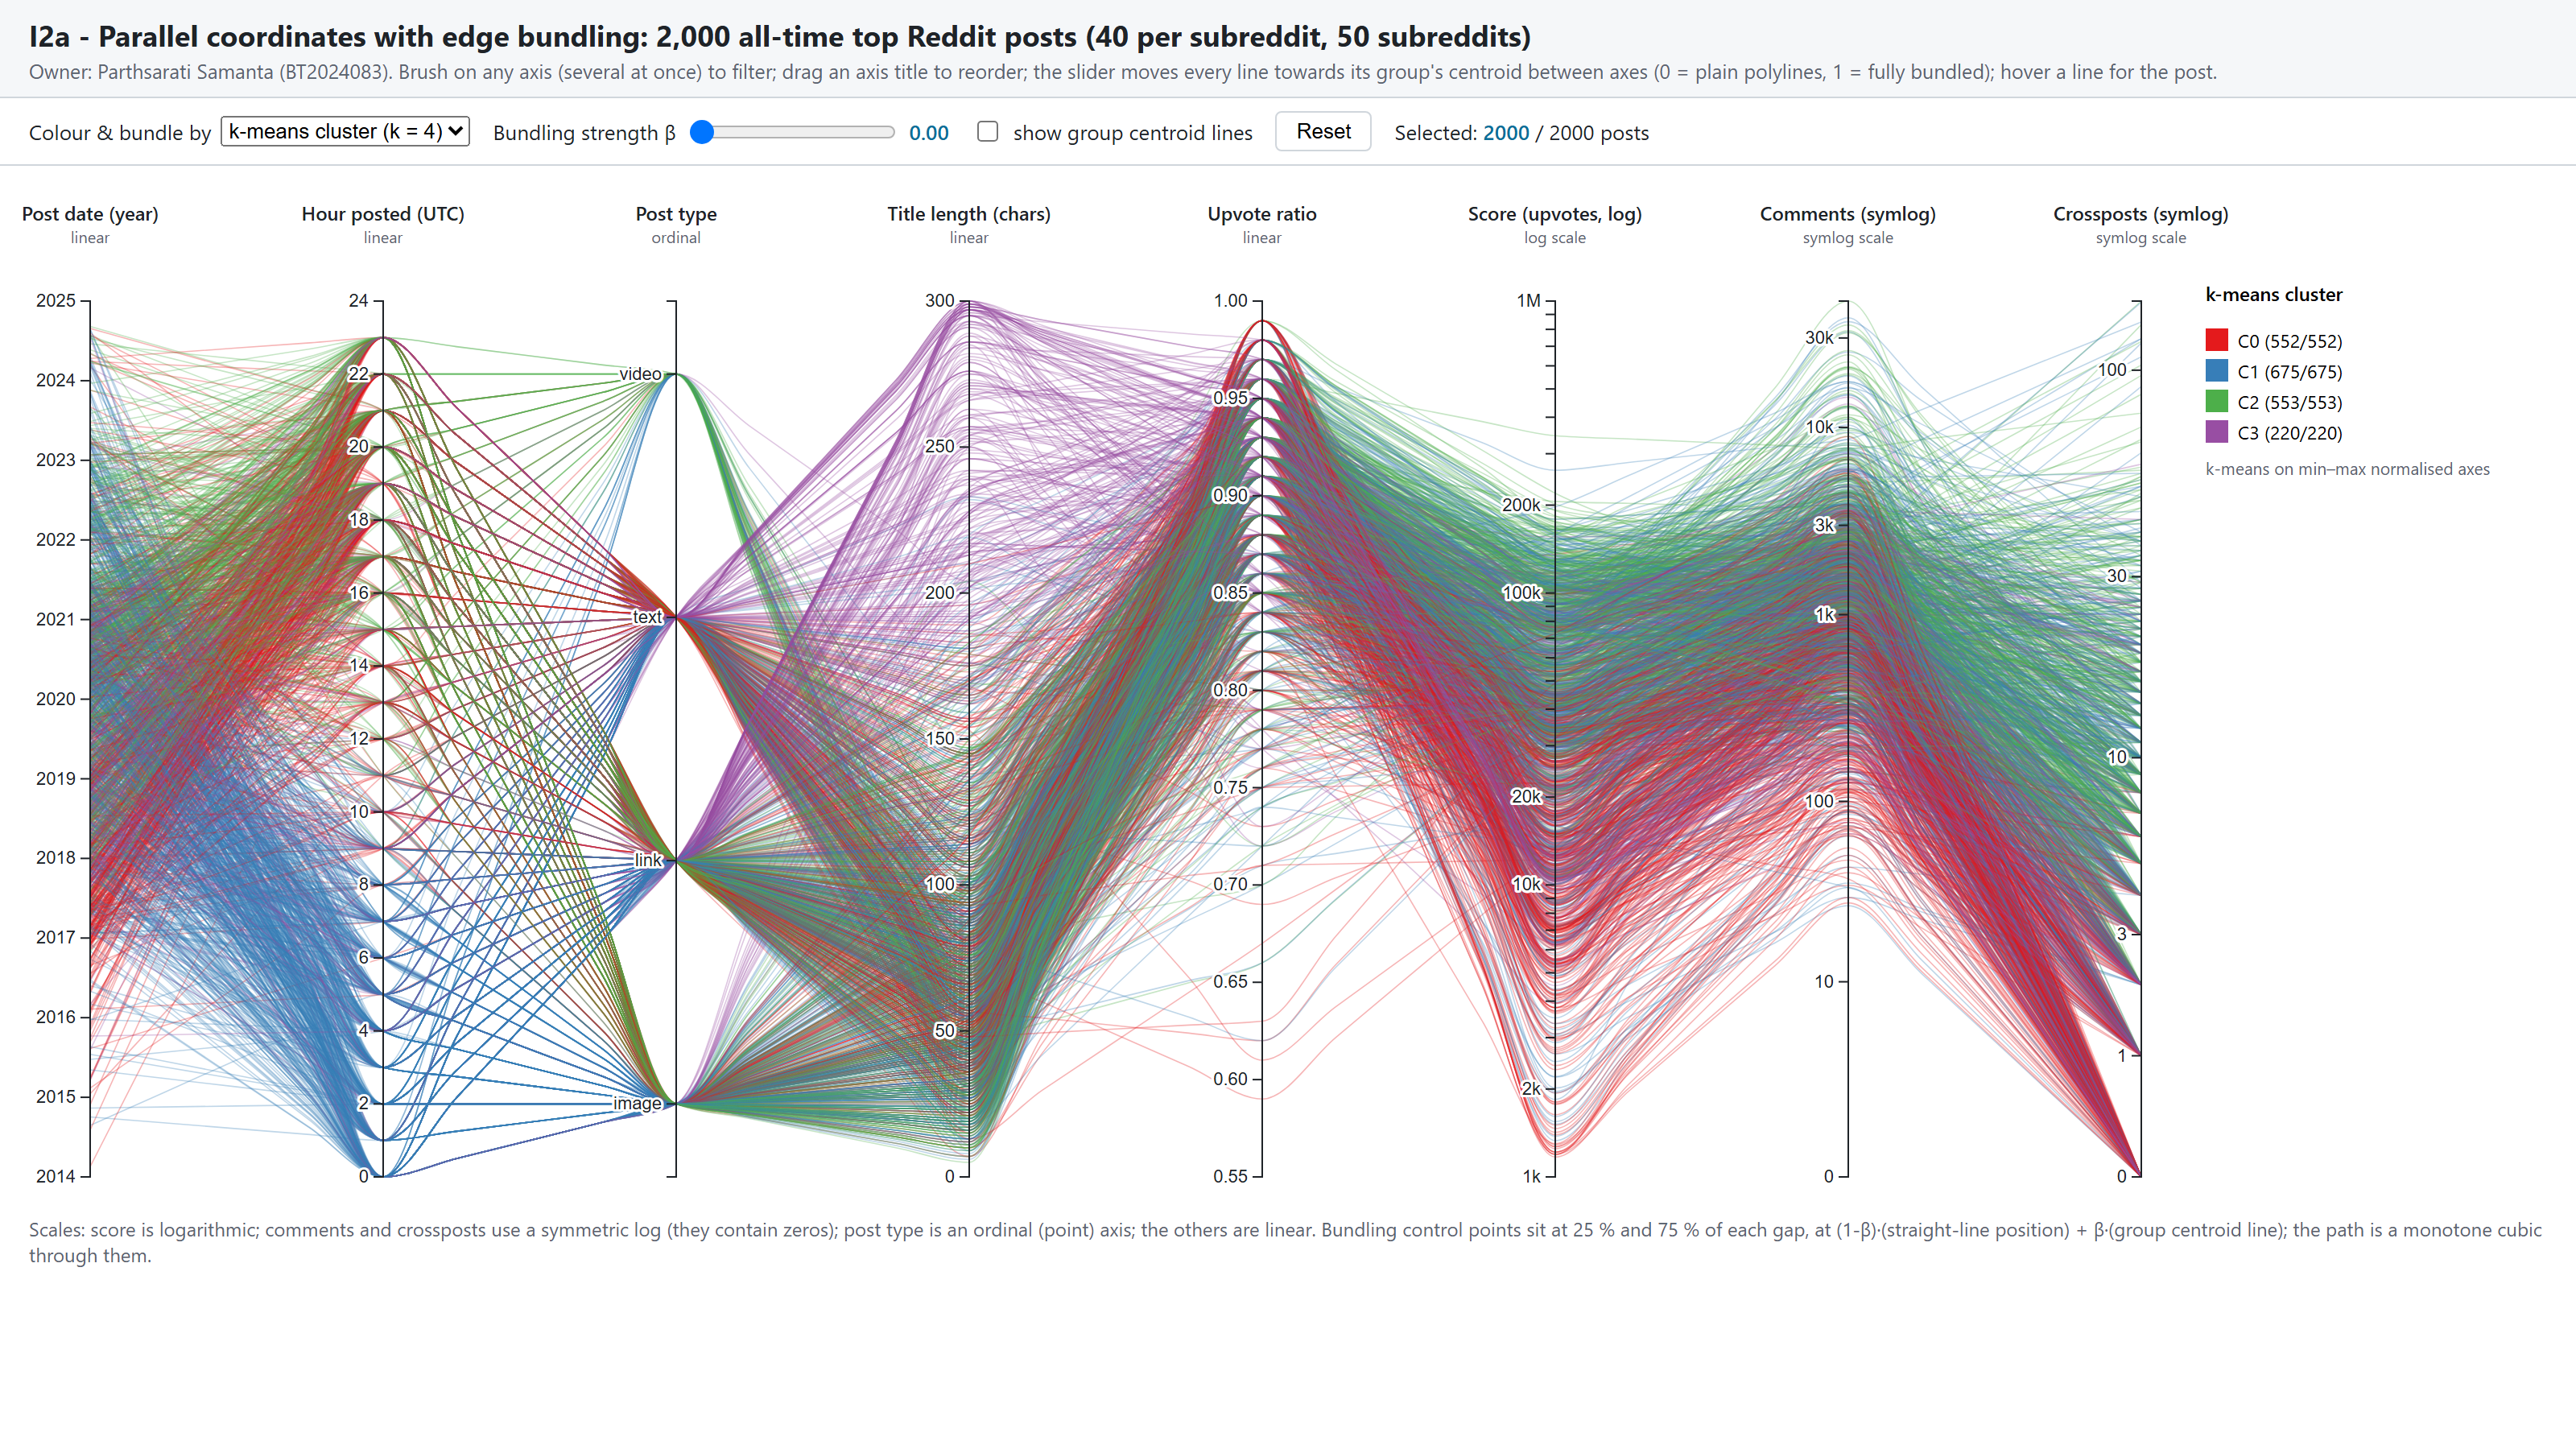
\includegraphics[width=0.495\textwidth]{Fig_31a_parcoords_unbundled.png}}\hfill
\subfloat[Bundled ($\beta=0.85$), k-means colour]{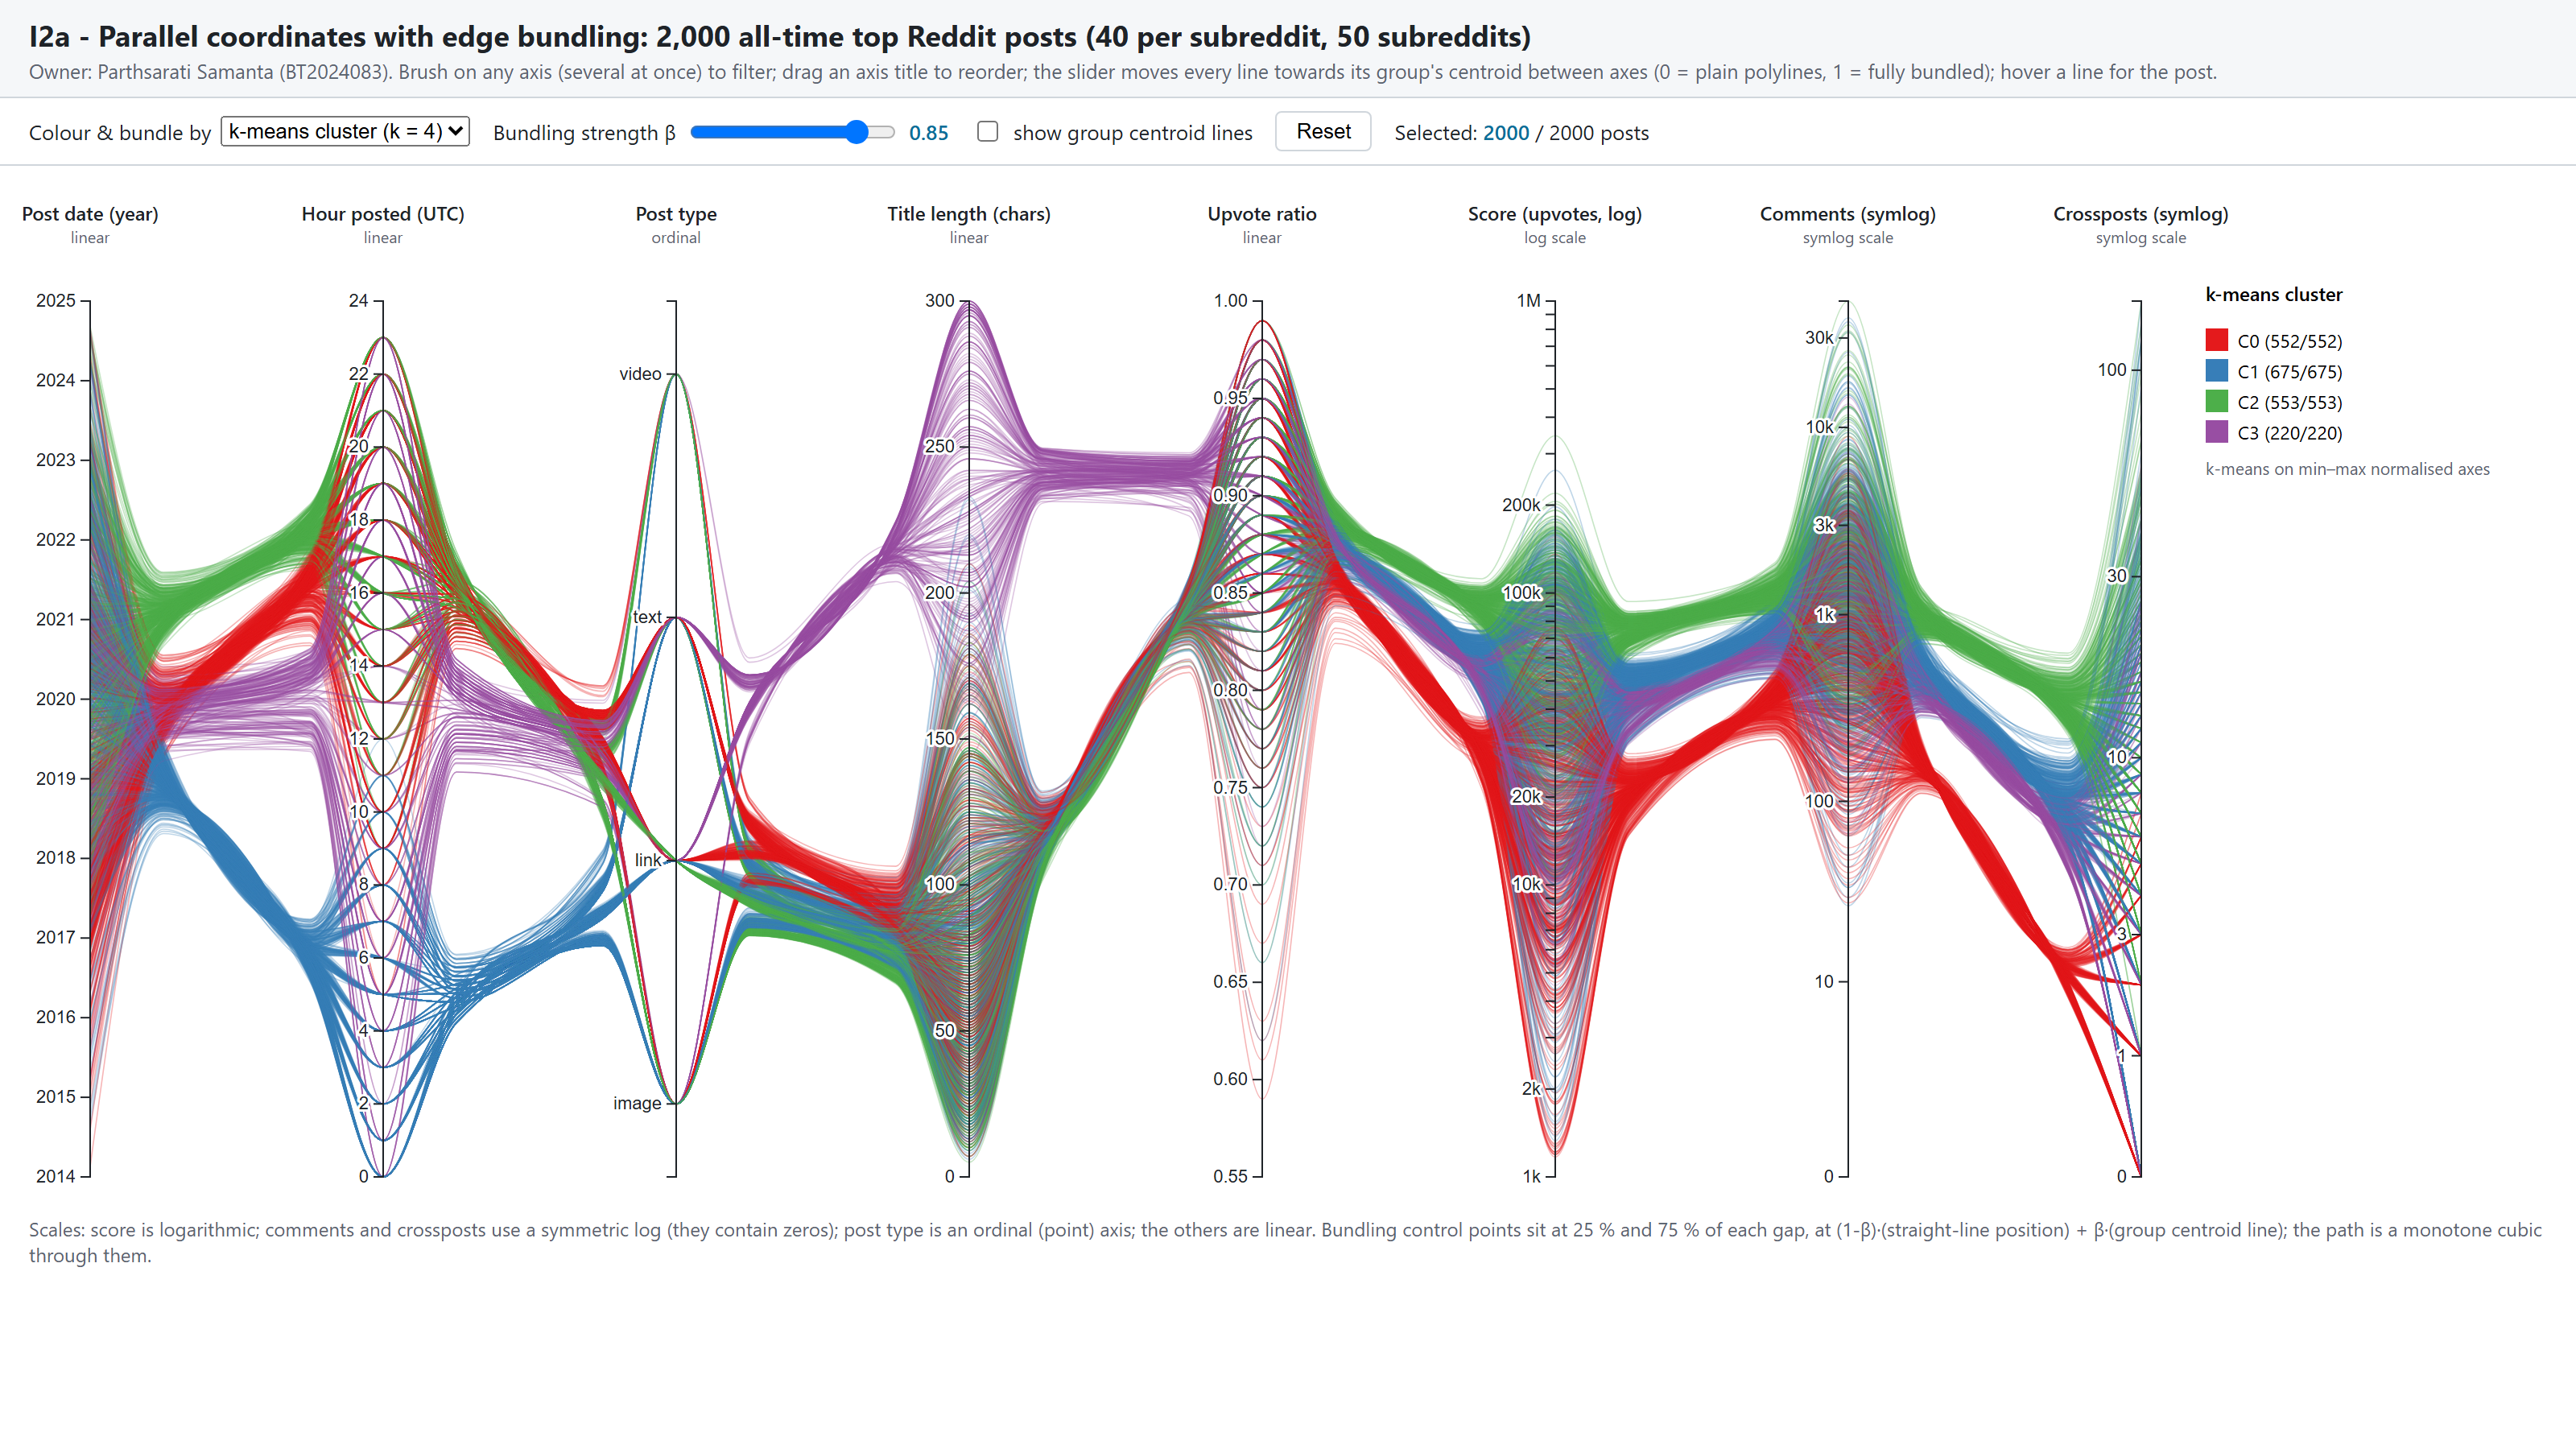
\includegraphics[width=0.495\textwidth]{Fig_31b_parcoords_bundled_kmeans.png}}\\
\subfloat[Bundled ($\beta=0.85$) by topic, with dashed centroid lines]{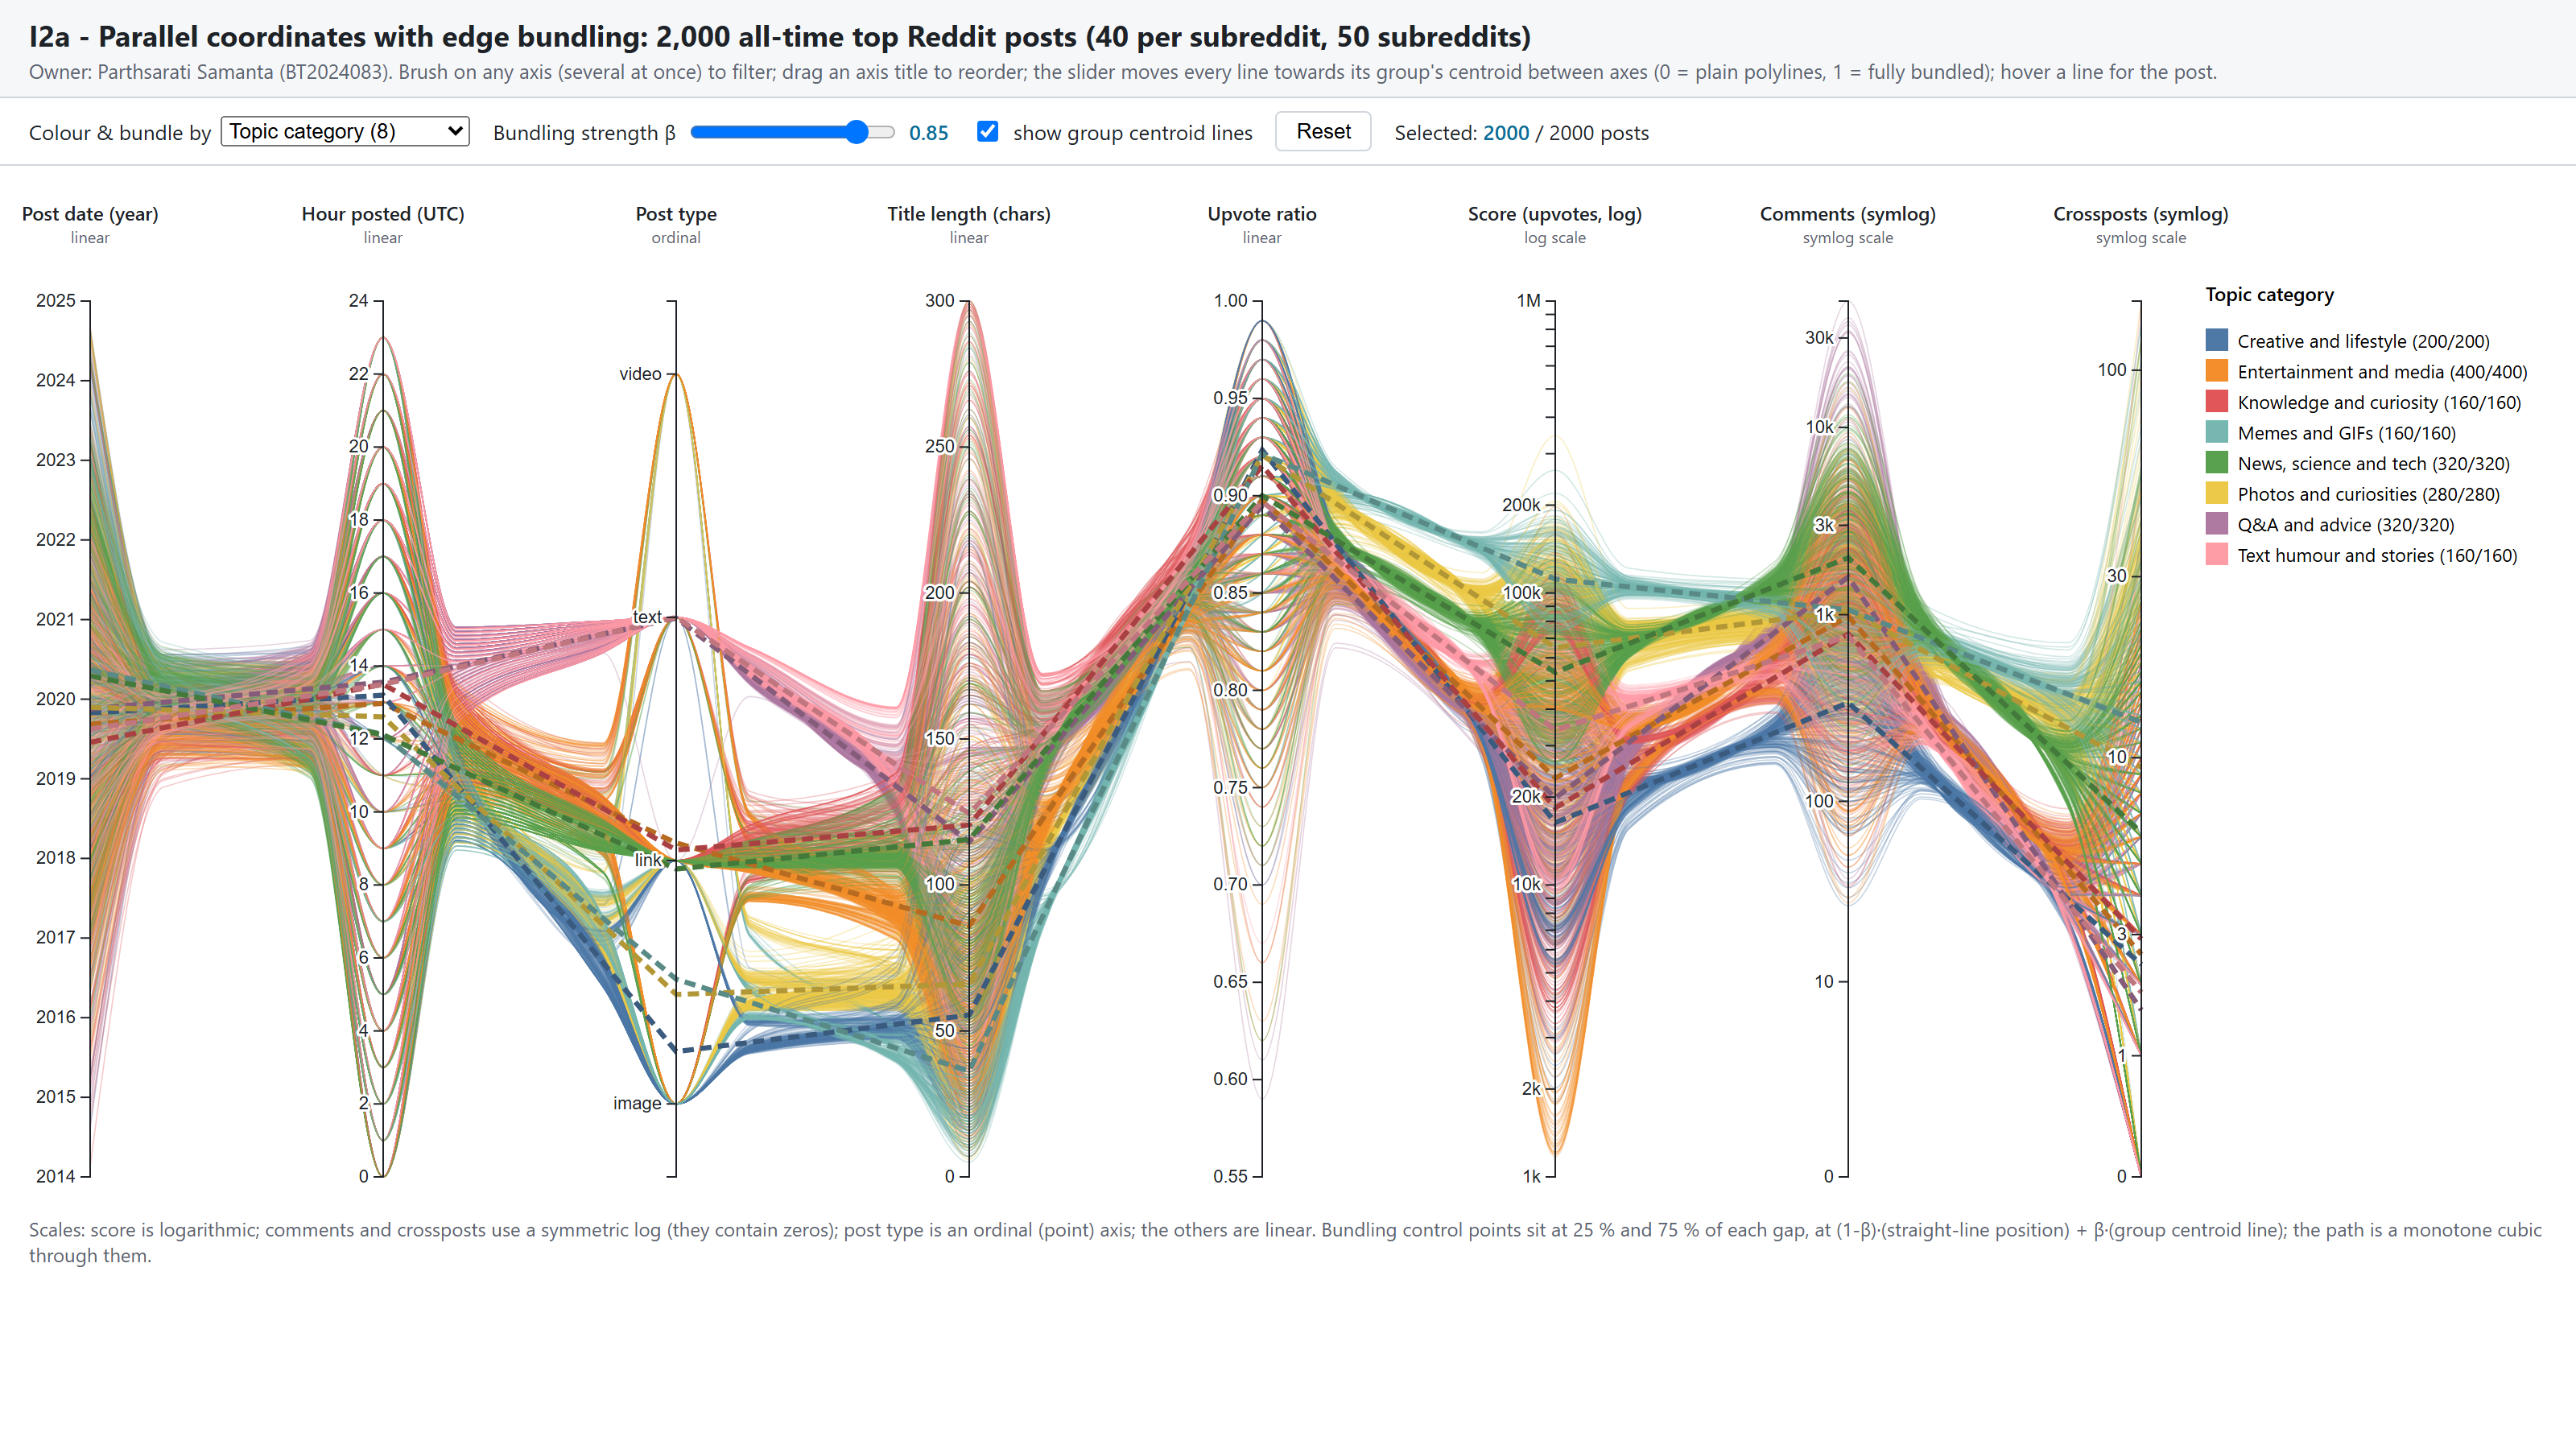
\includegraphics[width=0.495\textwidth]{Fig_31c_parcoords_bundled_topic.png}}
\caption{Parallel coordinates of 2,000 top posts: effect of edge bundling (I2a). Files \fpath{Fig_31a/b/c_*.png}.}
\label{fig:31}
\end{figure*}

\begin{figure*}[!t]
\centering
\subfloat[Brushes: score $\ge$60k AND post type = text; colour = post type]{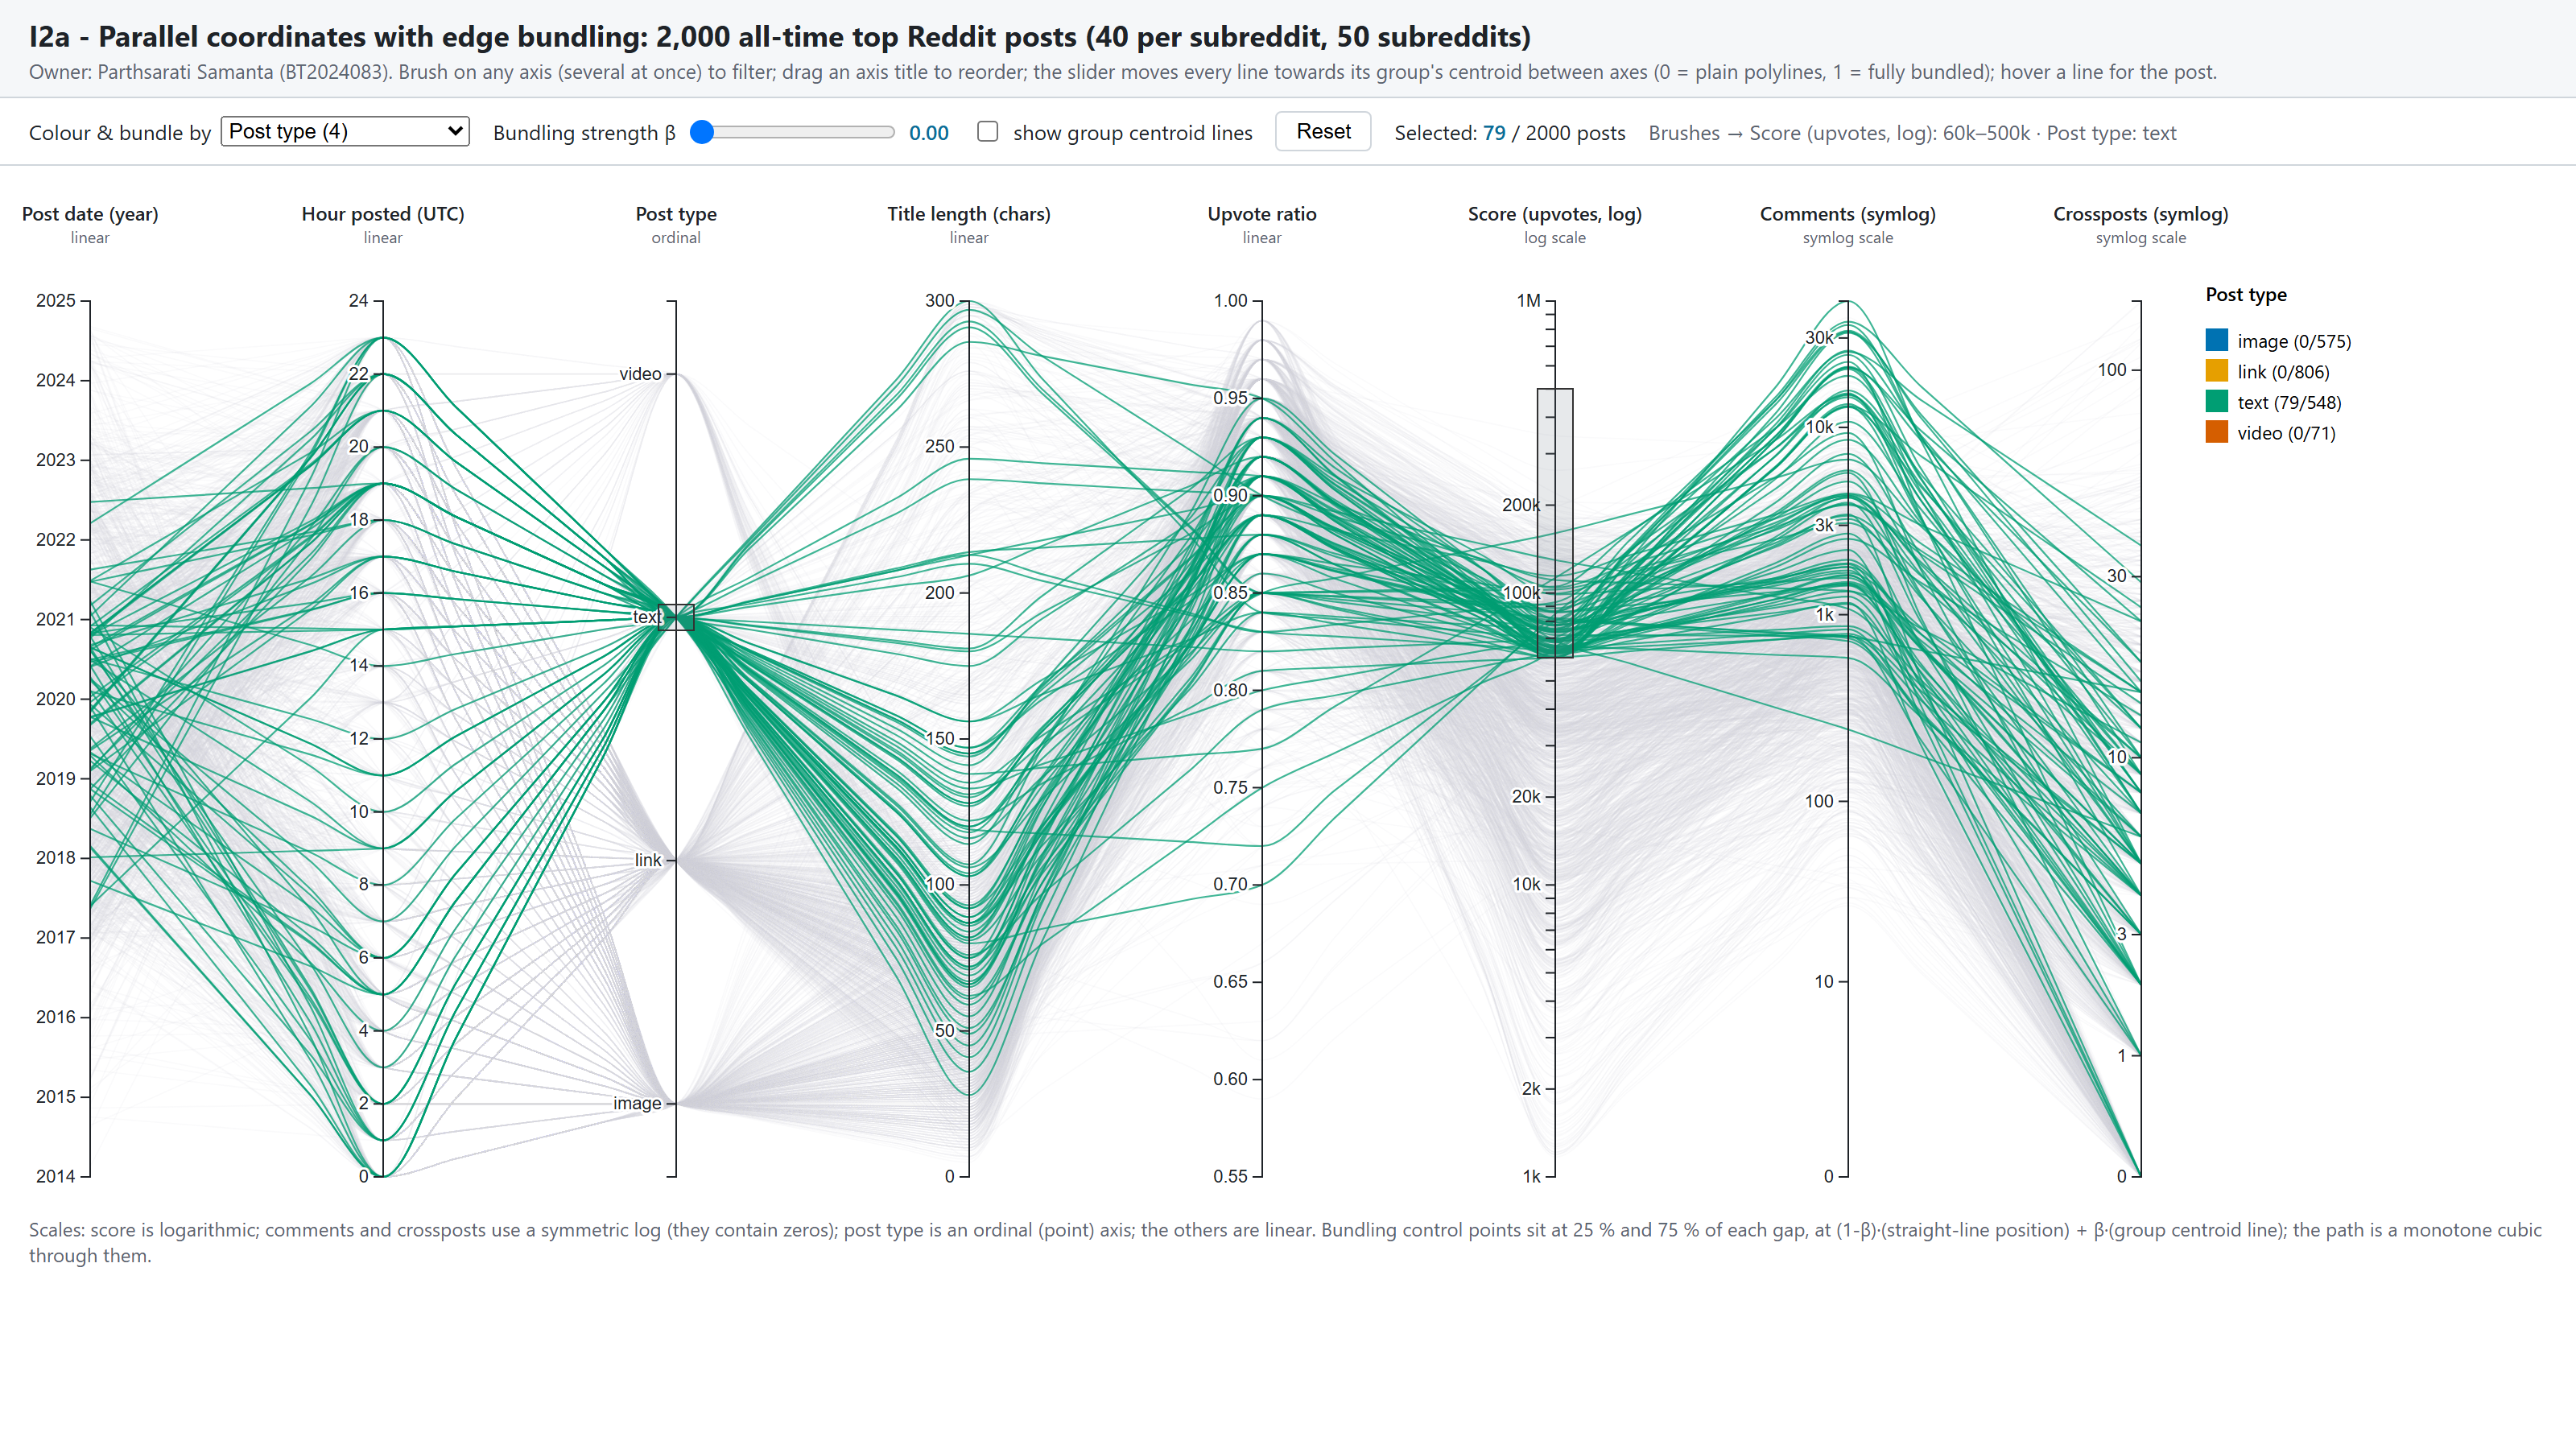
\includegraphics[width=0.495\textwidth]{Fig_32a_parcoords_brush_score_text.png}}\hfill
\subfloat[Brushes: comments $\ge$3,000 AND upvote ratio $\le$0.85; colour = topic]{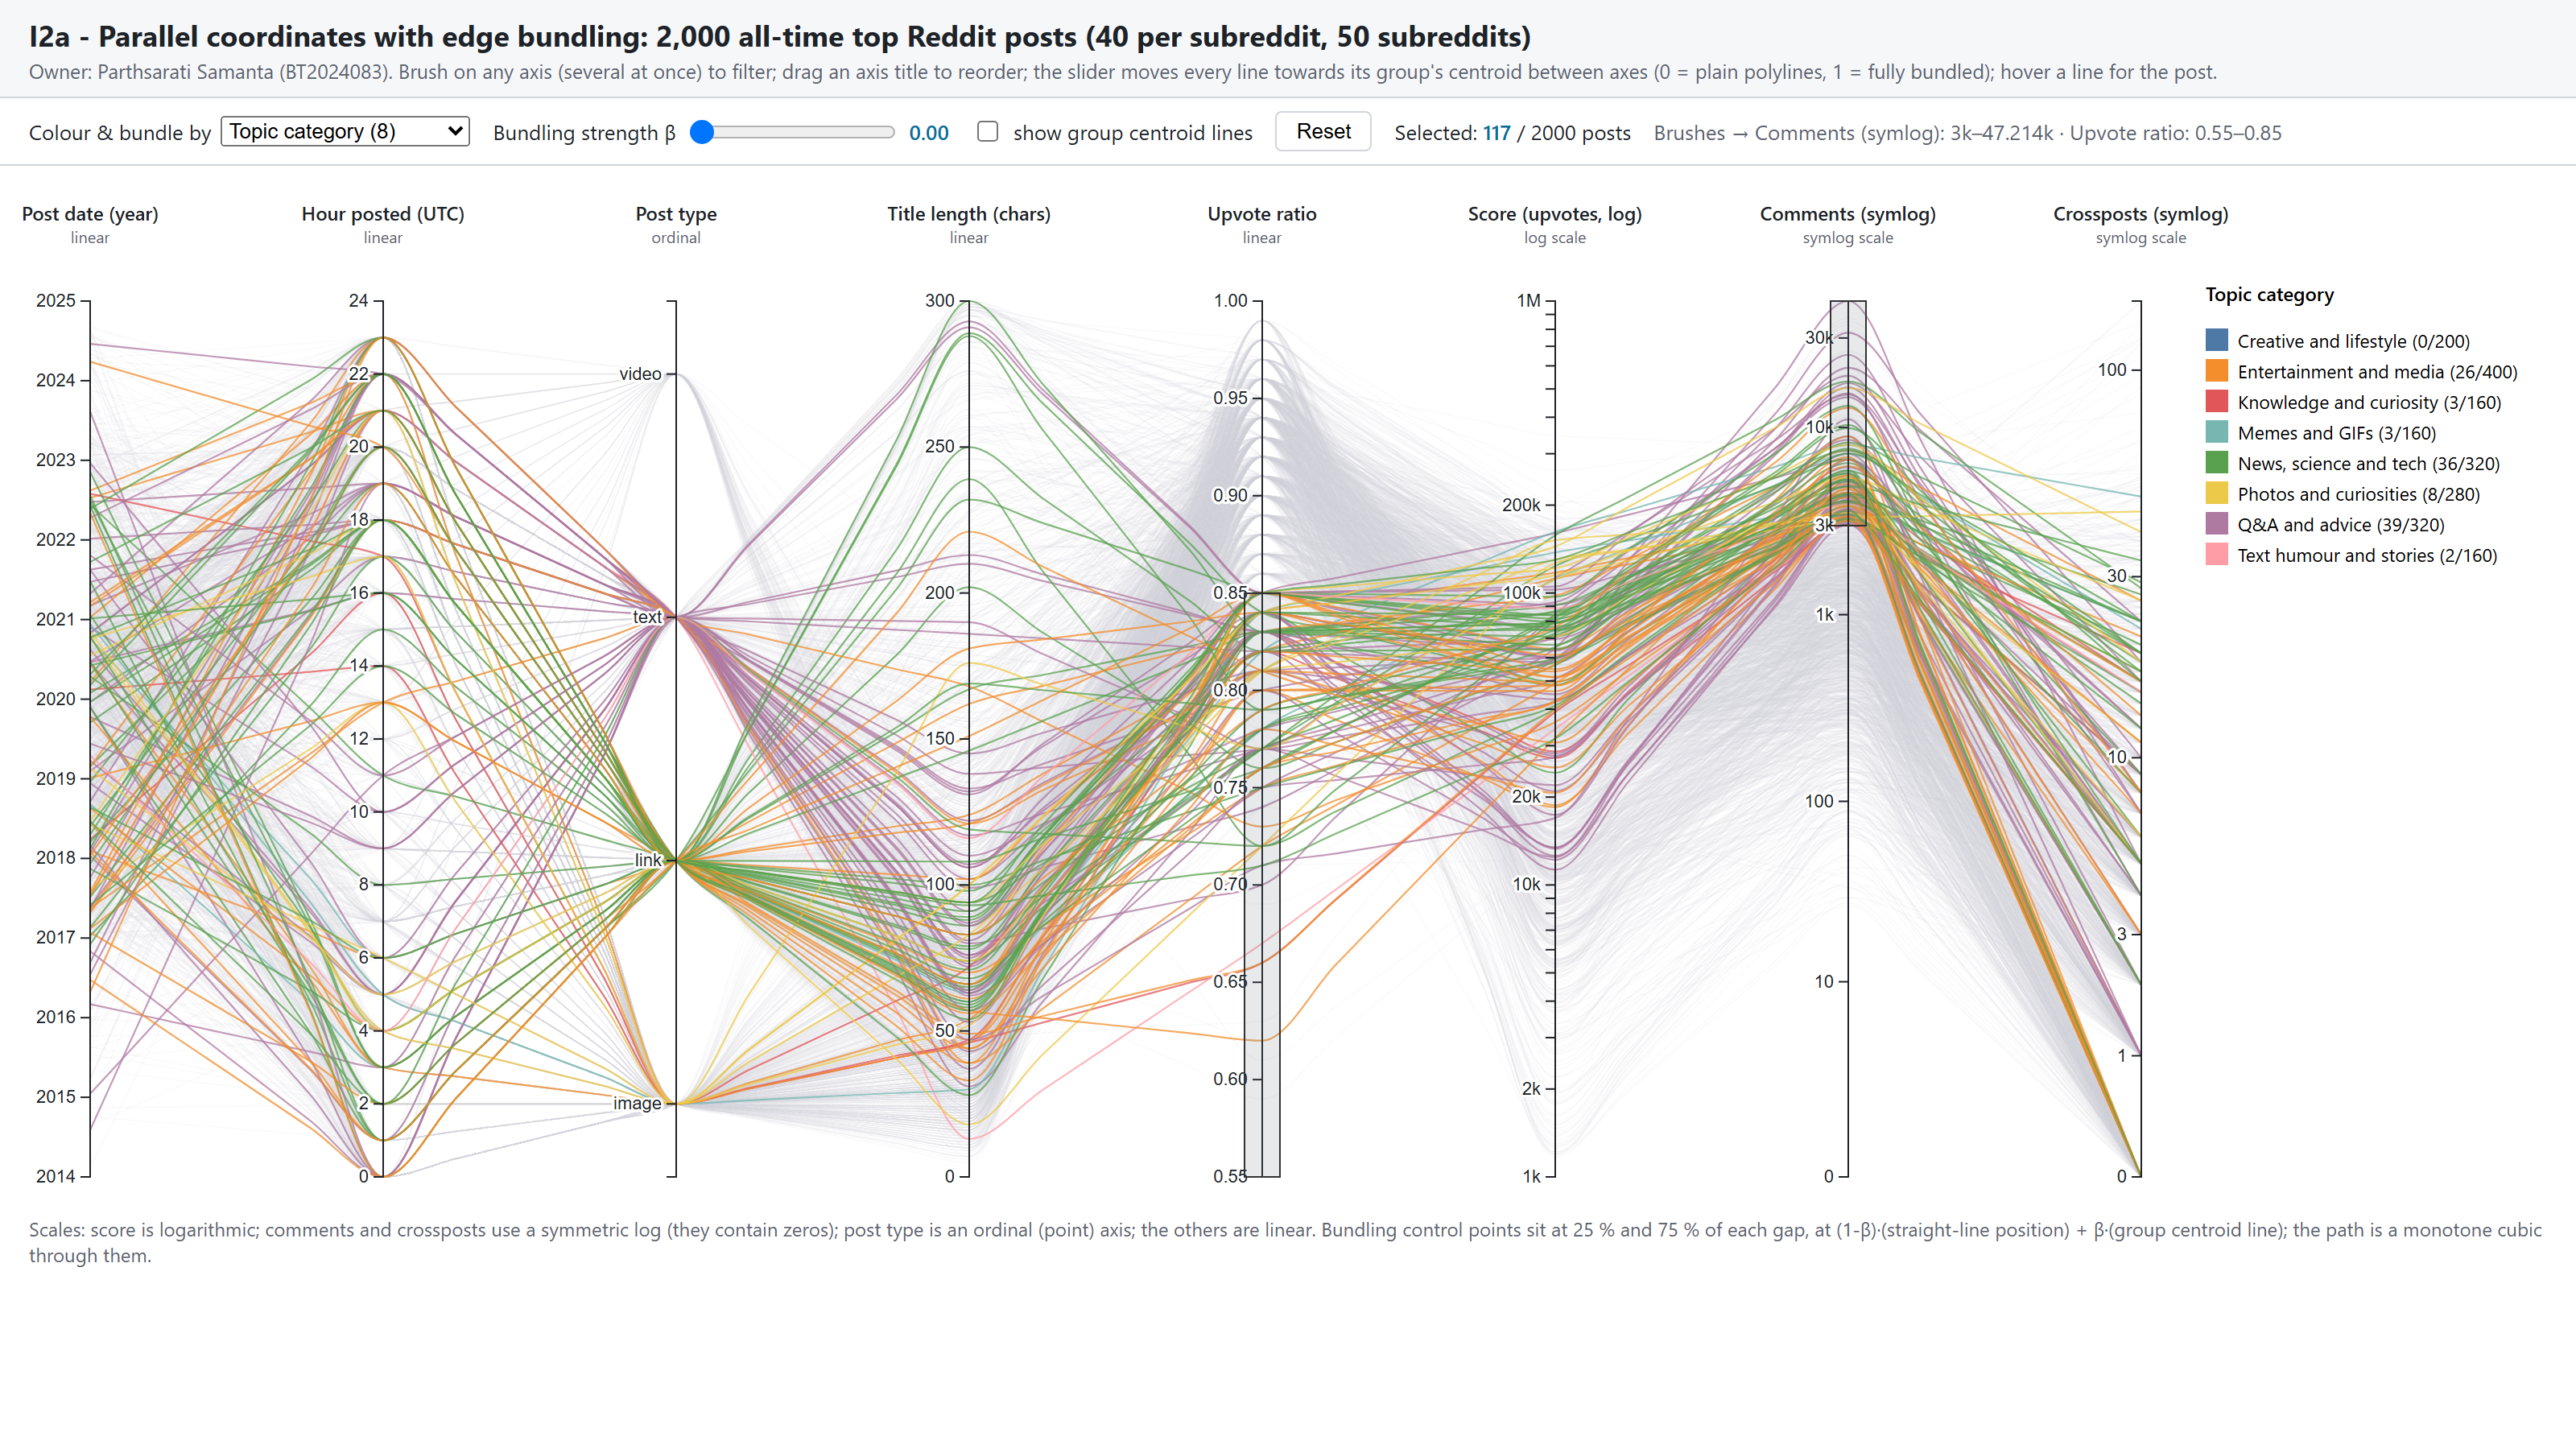
\includegraphics[width=0.495\textwidth]{Fig_32b_parcoords_brush_controversial.png}}\\
\subfloat[Axes reordered (post type first, date last), $\beta=0.5$, brush year $\ge$2021]{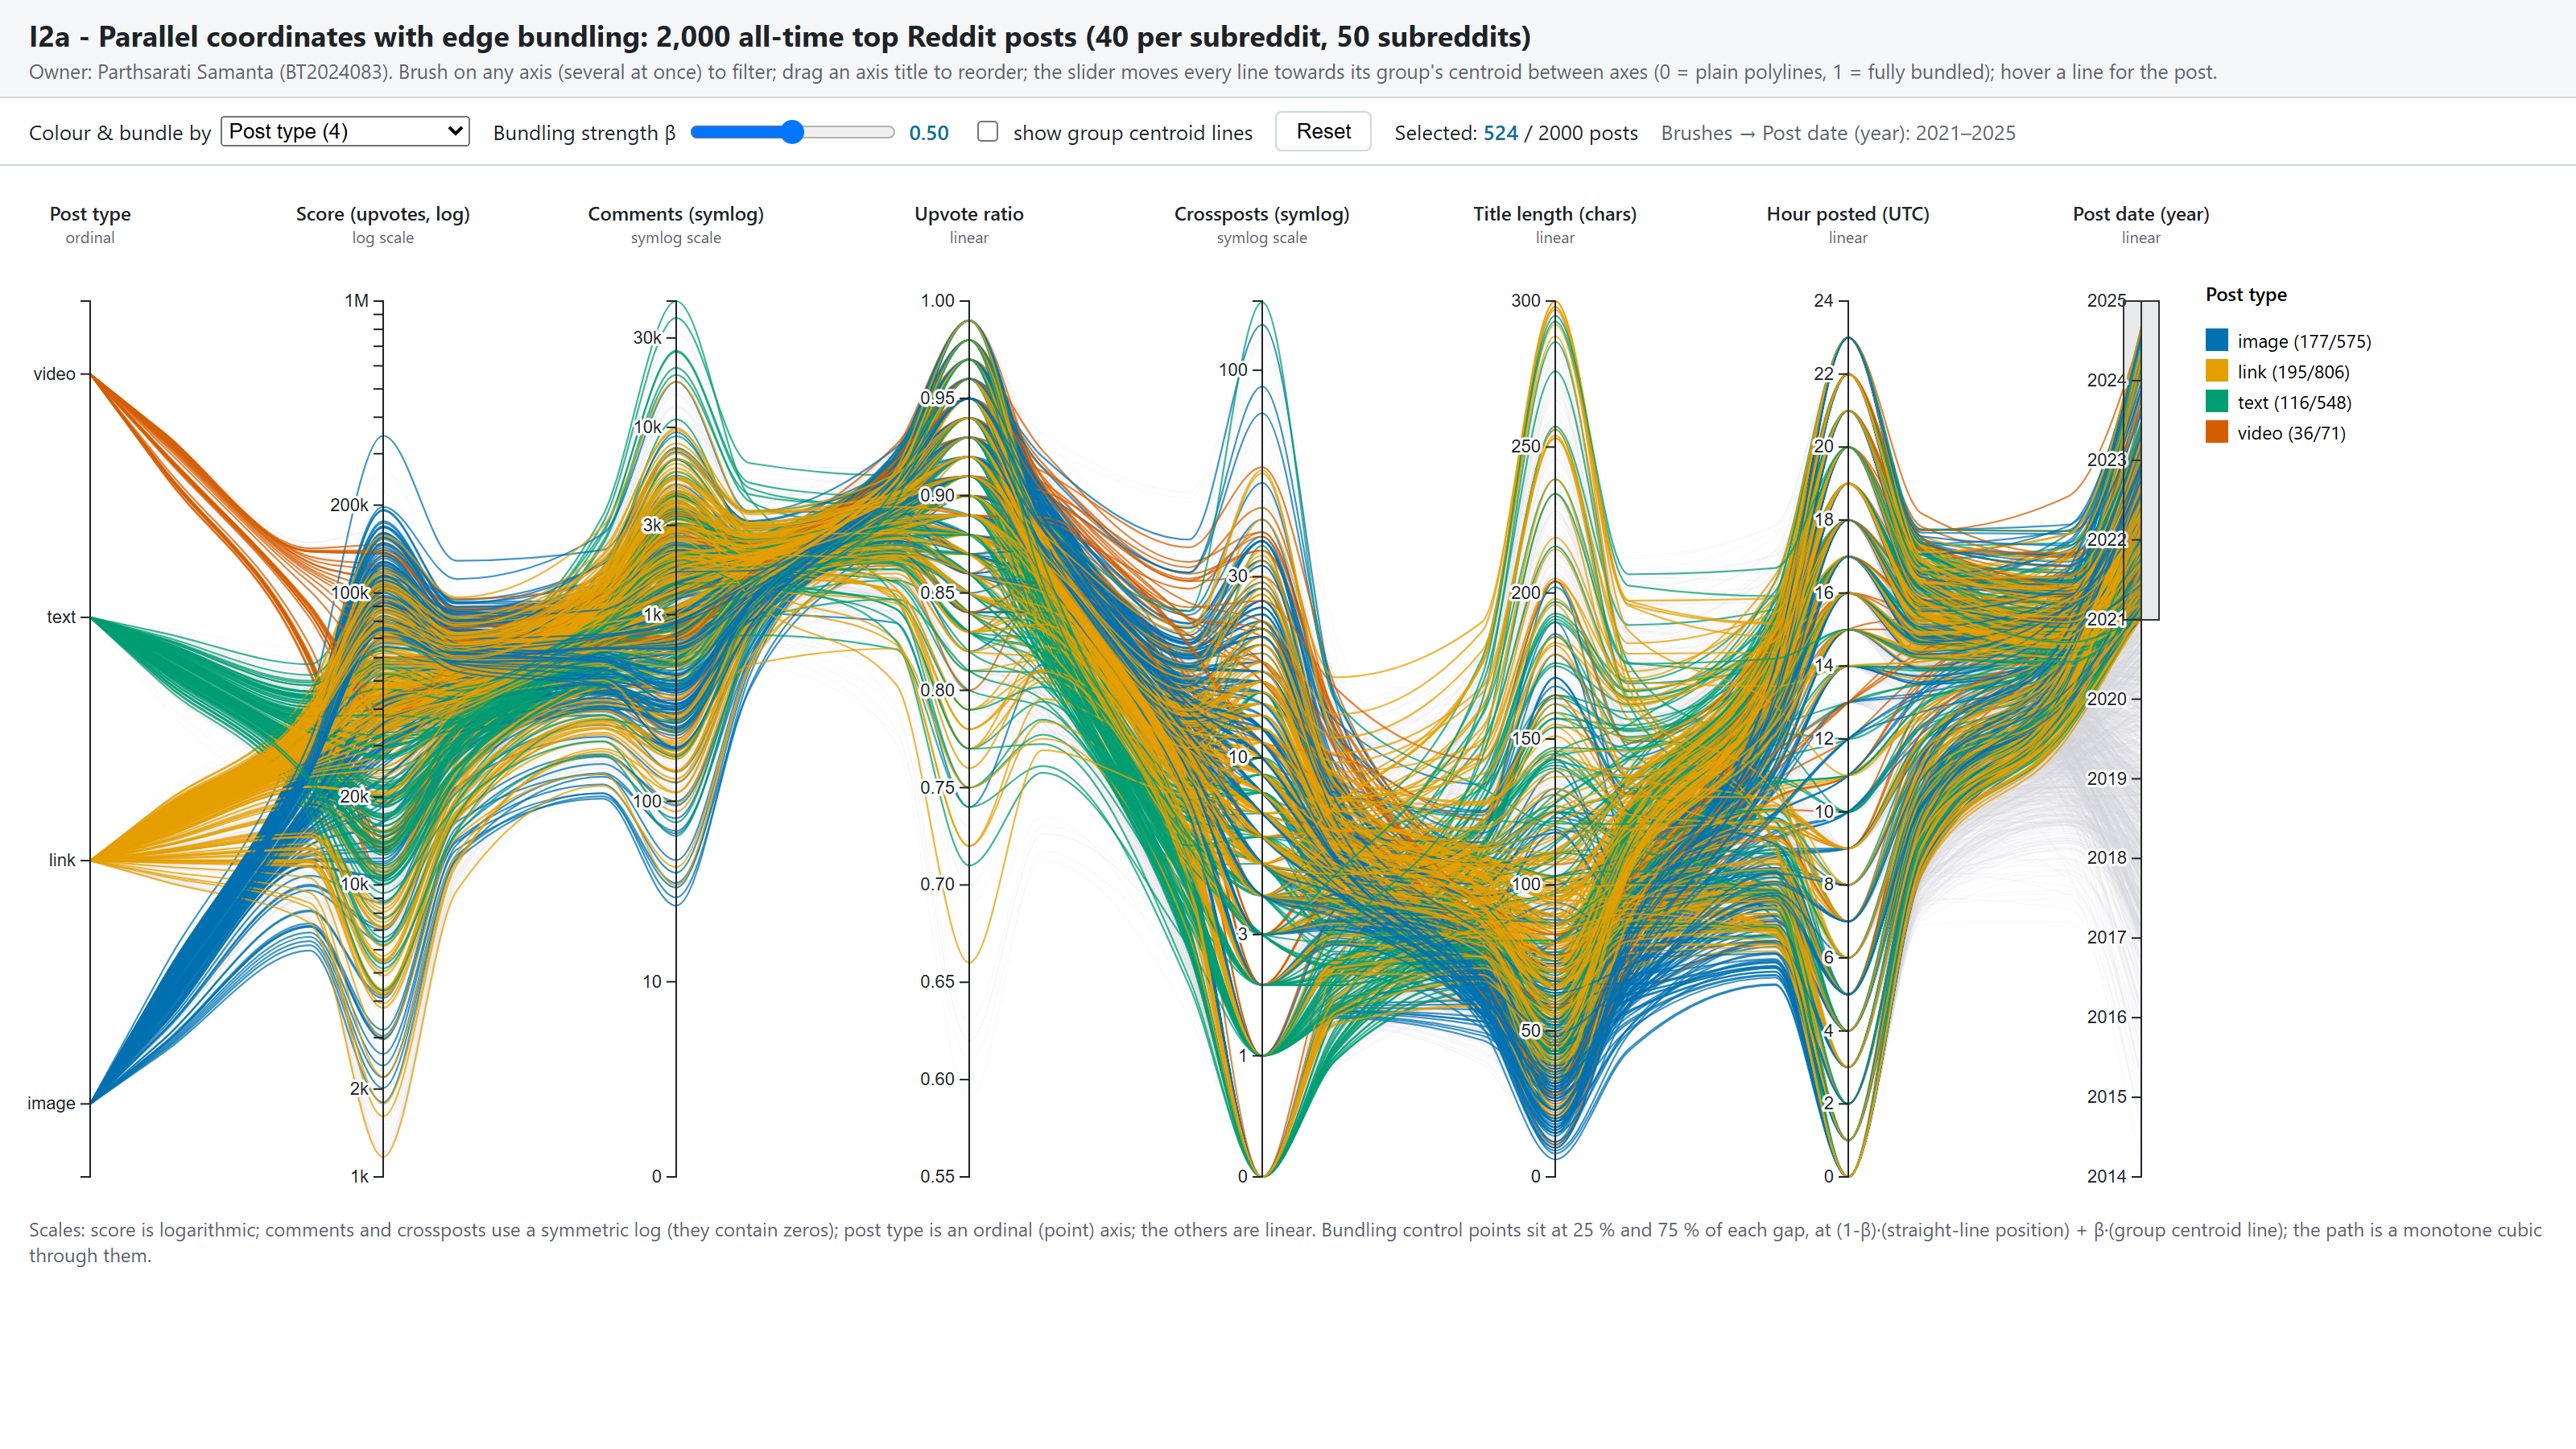
\includegraphics[width=0.495\textwidth]{Fig_32c_parcoords_reordered.png}}
\caption{Brushing and axis reordering (I2a). Files \fpath{Fig_32a/b/c_*.png}.}
\label{fig:32}
\end{figure*}

\input{generated/tab_pcstates}

\textbf{Inferences (bundling, Fig.~\ref{fig:31}).}
(1) Unbundled (Fig.~\ref{fig:31}a), 2,000 lines over eight axes form a dense ``hairball''. Only marginal patterns are
visible: hours cluster at 14--23 and 0--5 UTC (US daytime and evening), scores span 1k--400k, and most upvote ratios sit at
0.85--0.97.
(2) Bundling with $\beta=0.85$ (Fig.~\ref{fig:31}b) turns the four k-means clusters into four readable ribbons. C1 (675
posts) is the \emph{night-UTC} cluster (median hour 3 UTC, i.e.\ US evening) with medium score (median 43.9k). C2 (553) is
the \emph{high-performing evening} cluster (median hour 19 UTC, the highest median score 70.7k, 1,598 comments and 10
crossposts). C0 (552) has the same evening hours but is \emph{low-reach} (median score 14.9k, 0 crossposts). C3 (220) is
the \emph{long-title} cluster (median title of 242 characters against about 65 elsewhere), mostly link and text posts.
Hour and crossposts, not topic, drive the clustering. That explains the low silhouette (0.248): the clusters are bands in a
continuum.
(3) Bundling by topic (Fig.~\ref{fig:31}c) with centroid lines shows that Q\&A and text communities sit at the
\emph{text} position of the post-type axis with low crossposts, while image communities (Photos, Memes) have the highest
centroid scores. Ribbon crossings between axes show negative relations, such as upvote ratio against comments.
(4) The cost of bundling is fidelity between axes. At high $\beta$ the line segments between two axes no longer show the
individual pairwise relation, and outliers within a group are pulled into the ribbon. We therefore keep the slider
and read individual records at $\beta=0$.

\textbf{Inferences (brushing and reordering, Fig.~\ref{fig:32}, Table~\ref{tab:pcstates}).}
(1) Brushing score $\ge$60k selects 654 posts (33\,\%): link 276, image 262, text 79, video 37. Adding post type = text
leaves 79 posts, of which 32 are from AskReddit, 27 from Showerthoughts and 9 from LifeProTips (Fig.~\ref{fig:32}a). Text
posts reach the very top almost only in three ``prompt'' communities, and their titles are short (Showerthoughts and
AskReddit questions).
(2) Brushing comments $\ge$3,000 \emph{and} upvote ratio $\le$0.85 isolates 117 \emph{controversial discussions} (median
ratio 0.82). They come from AskReddit (16), news (12), IAmA (11), videos (9) and Futurology (8). The brush shows the
negative association between agreement and discussion that the data confirm (Spearman $\rho=-0.45$ between upvote ratio
and comments): posts people argue about collect comments but fewer net upvotes.
(3) Reordering the axes to post type, score, comments, ratio, crossposts, title, hour, date (Fig.~\ref{fig:32}c) puts
related axes next to each other. Post type next to score shows that image and link posts dominate the top of the score
axis. Score next to comments shows a positive fan (Spearman 0.55). With year $\ge$2021 brushed on the now-rightmost date
axis, the 524 recent posts are 6.9\,\% video against 3.6\,\% overall, and 33.8\,\% image against 28.8\,\%, while text falls to
22.1\,\% from 27.4\,\%. This is the post-2020 shift towards native media, also seen in the treemap (Fig.~\ref{fig:33}).

\subsection{I2b: Zoomable treemap}
\textbf{Design.} We follow the zoomable-treemap pattern~\cite{shneiderman1992,bostock_zoomtreemap}. Every node's
children are laid out in the \emph{full viewport} with the chosen tiling and then scaled into the parent's rectangle. A
zoomed level therefore keeps the tiling's aspect-ratio behaviour at screen size (code in Appendix~\ref{app:code}).
\begin{itemize}
\item \emph{Zoom}: clicking a node zooms in with a 750\,ms transition; the breadcrumb or the header bar zooms out.
\item \emph{Next level}: thin white outlines show the next level inside each child.
\item \emph{Labels}: fitted (truncated with an ellipsis) and placed on opaque label plates so outlines never cross text.
\item \emph{Tooltips}: value, share of the parent and share of the whole.
\item \emph{Dropdowns}: three hierarchy remodels (H1--H3), three size measures (posts, total score, total comments), five
  tilings (squarify~\cite{bruls2000}, binary, slice, dice, slice-dice) and two sort orders (by size, by name).
\item \emph{Colour}: stable across remodels. Topic, post type, hosting class and era each have a fixed palette, years use
  viridis, and subreddits use shades of their topic colour.
\item \emph{Metrics line}: the mean, median and maximum aspect ratio of the current view, and the Kendall $\tau$ between
  the sort order and the reading order, as a measure of order preservation.
\end{itemize}

\begin{figure*}[!t]
\centering
\subfloat[H1 topic$\rightarrow$subreddit$\rightarrow$type, size = posts]{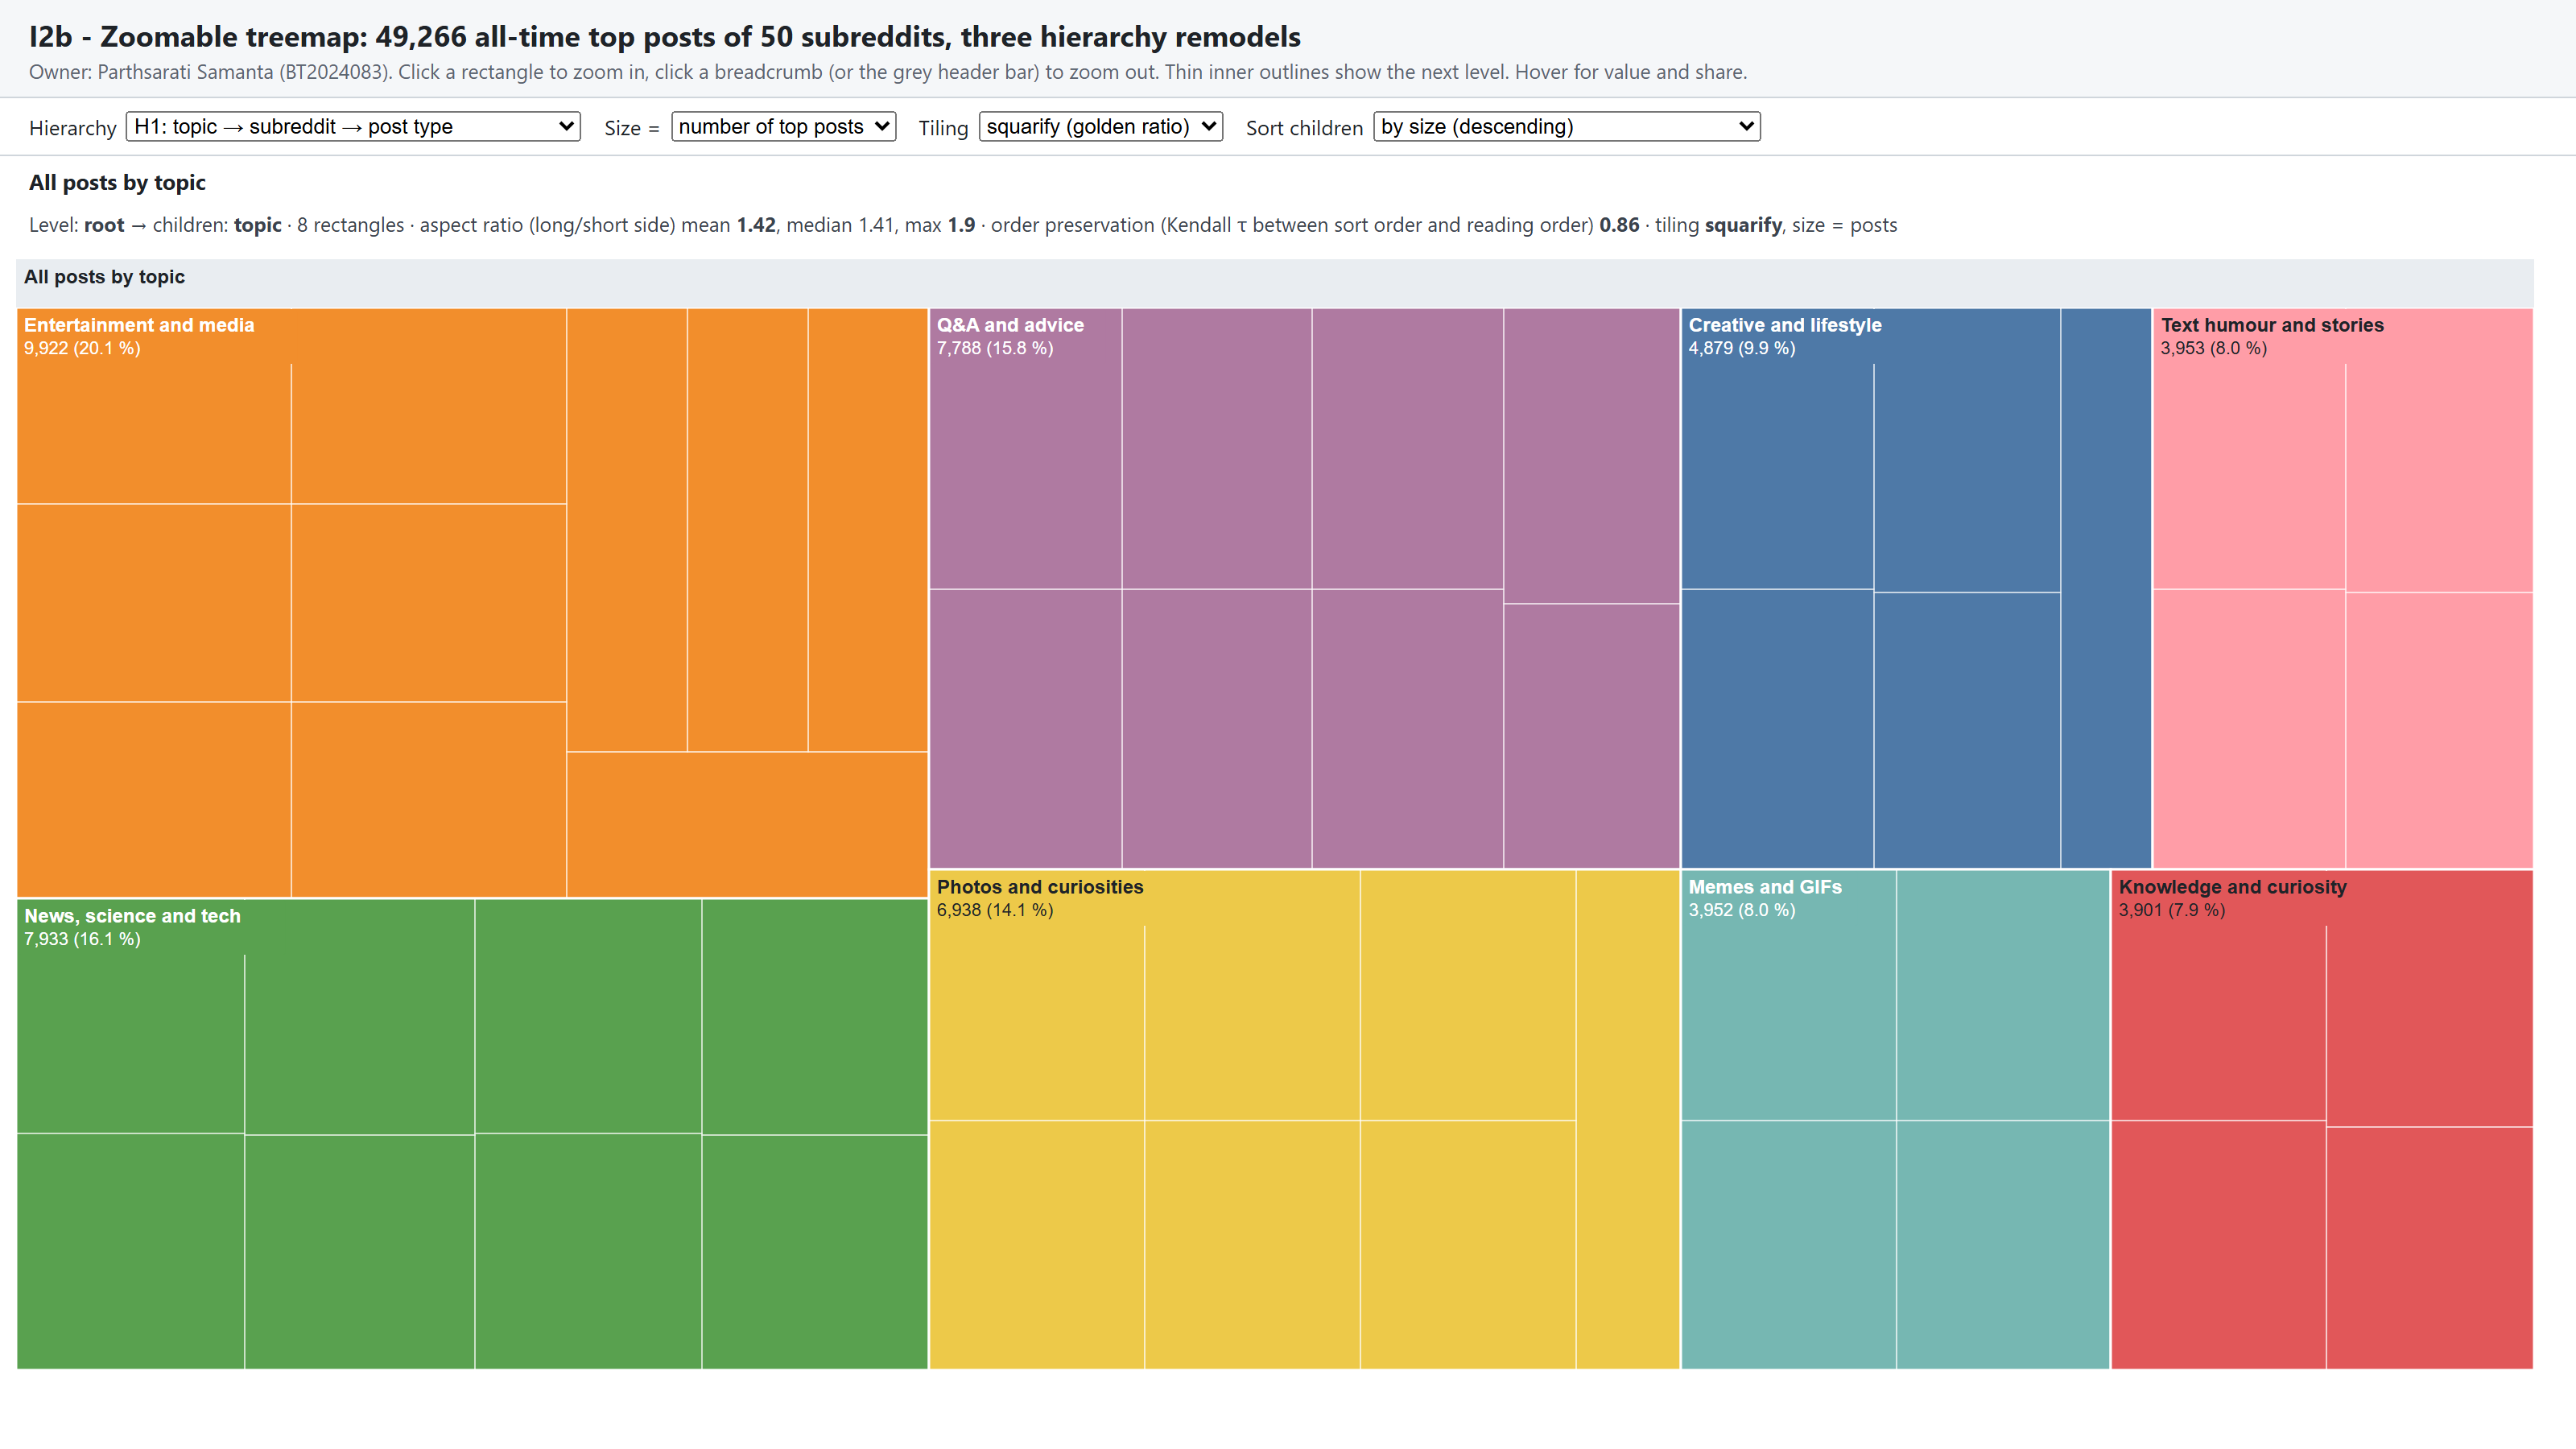
\includegraphics[width=0.495\textwidth]{Fig_33a_treemap_h1_topic.png}}\hfill
\subfloat[H2 post type$\rightarrow$hosting$\rightarrow$topic$\rightarrow$subreddit, size = posts]{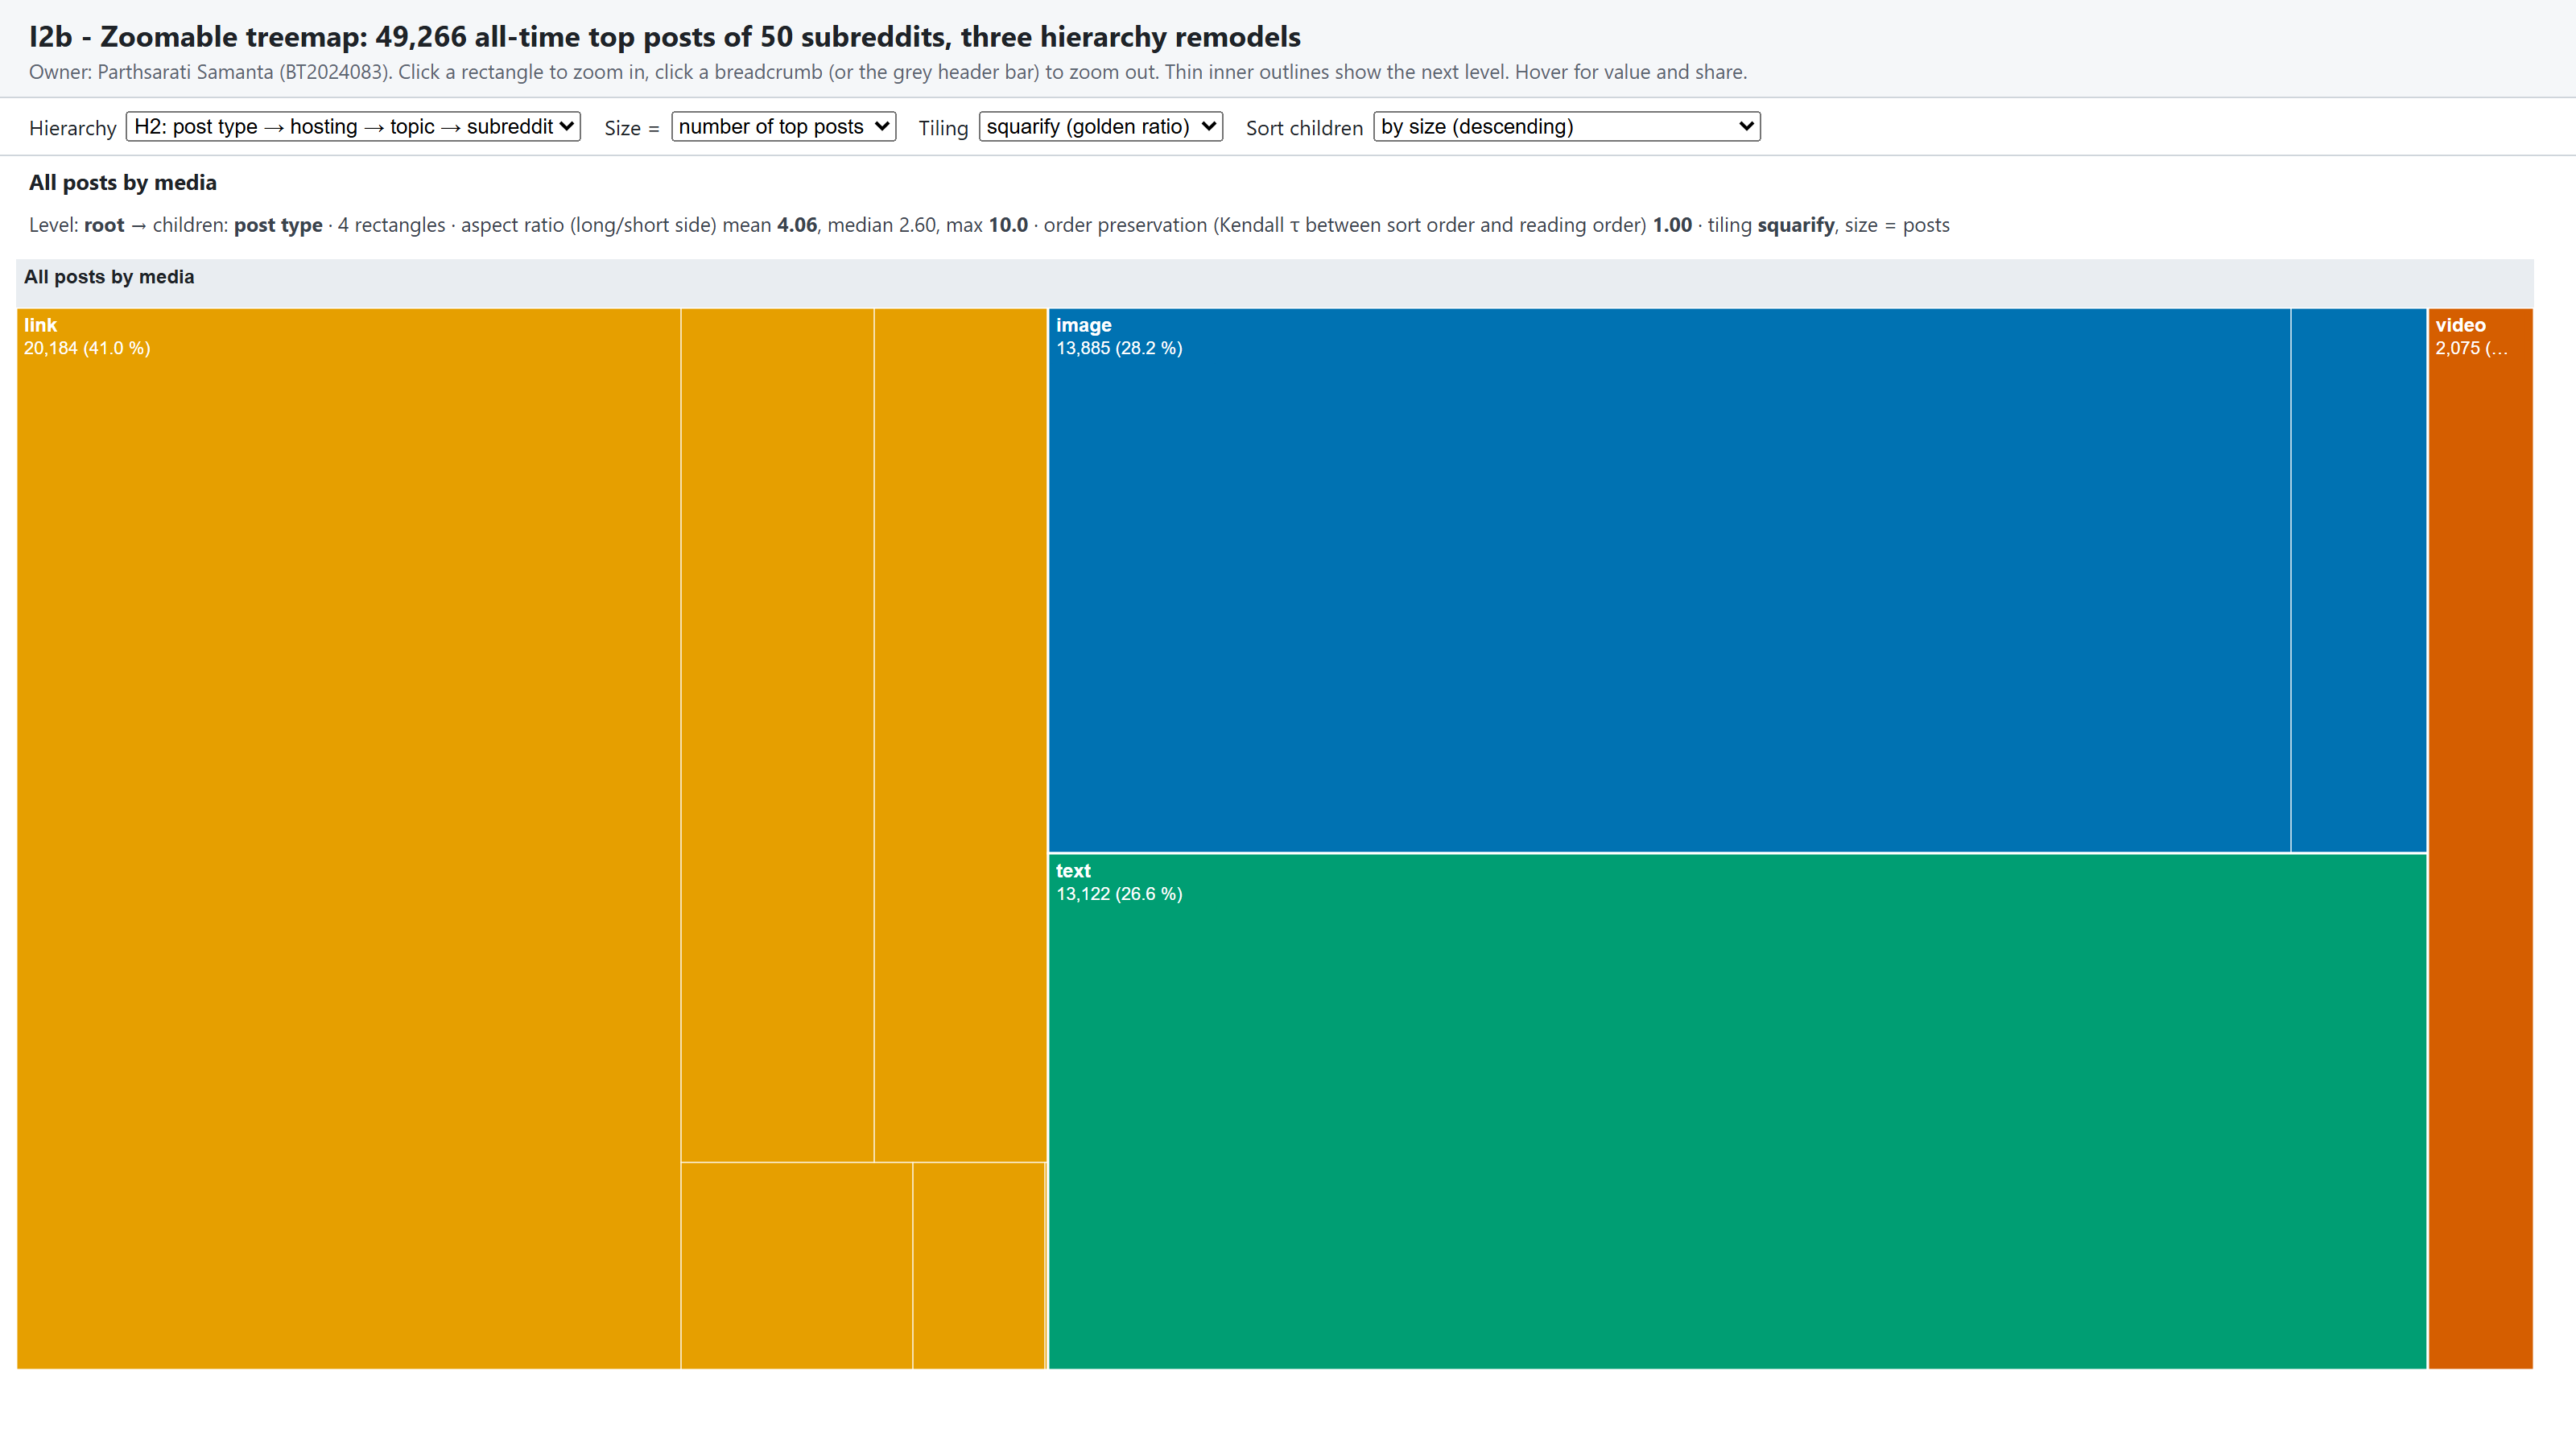
\includegraphics[width=0.495\textwidth]{Fig_33b_treemap_h2_media.png}}\\
\subfloat[H3 era$\rightarrow$year$\rightarrow$topic$\rightarrow$subreddit, size = posts]{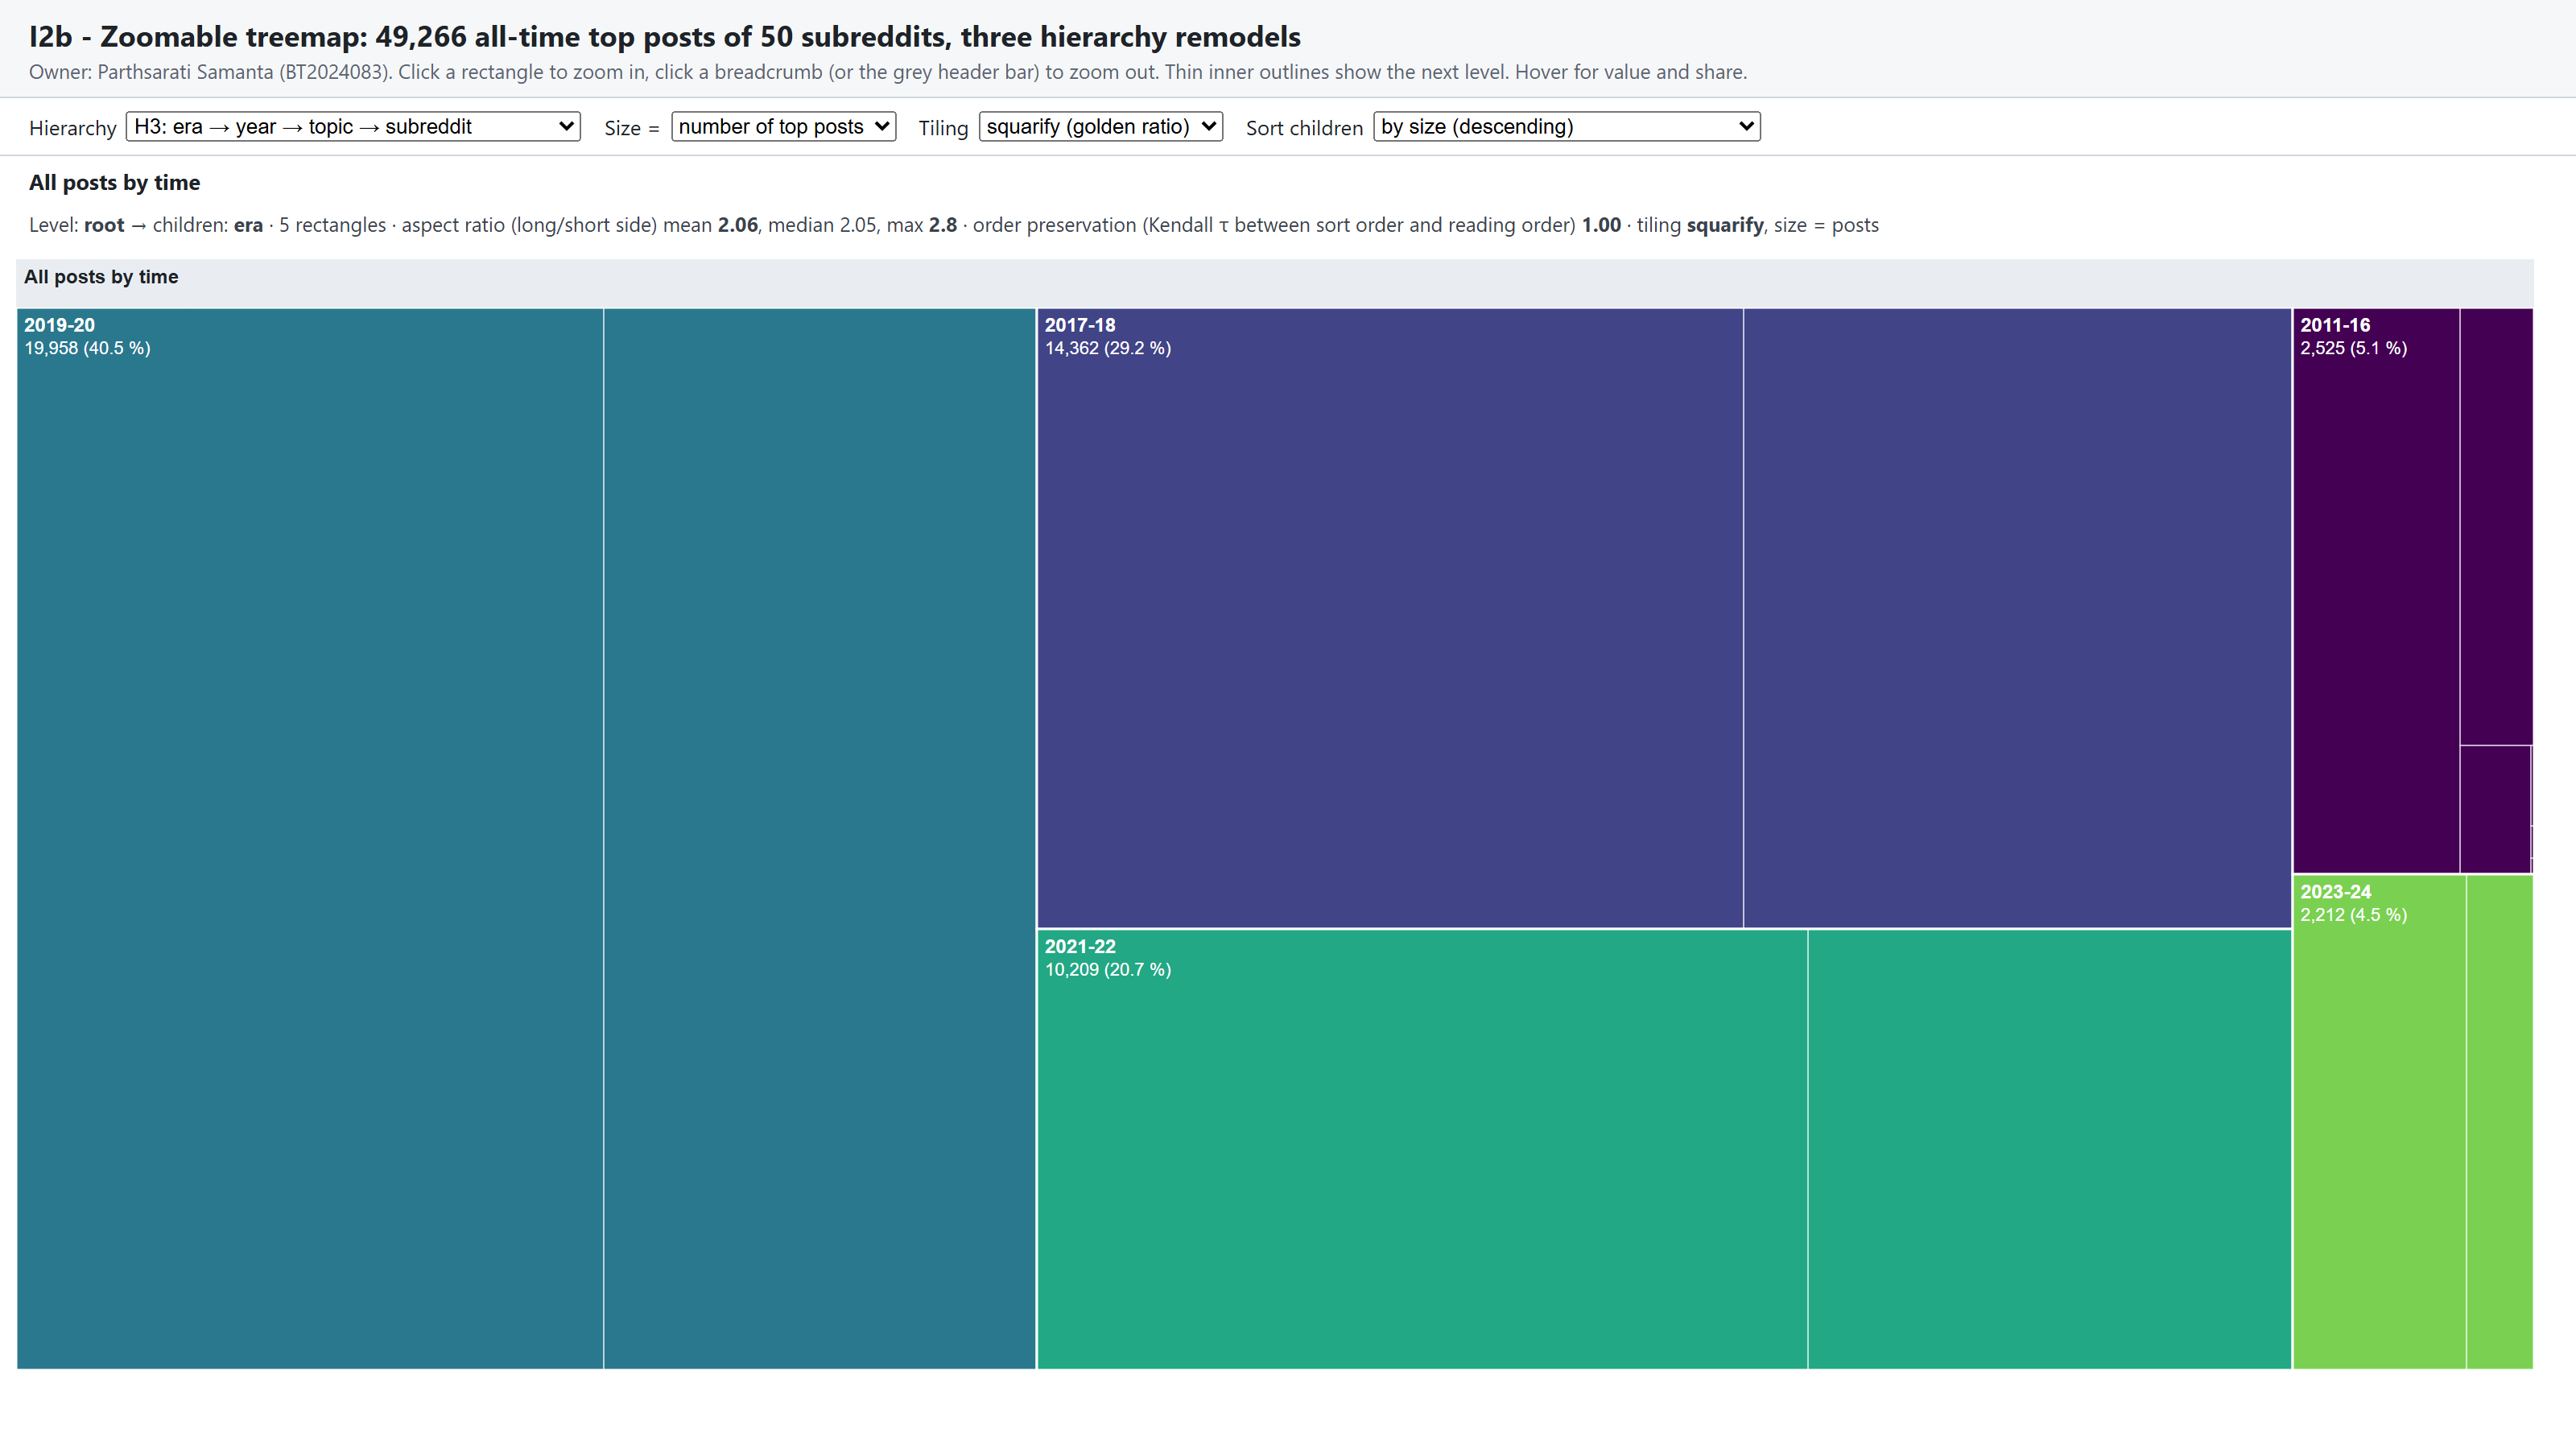
\includegraphics[width=0.495\textwidth]{Fig_33c_treemap_h3_time.png}}\hfill
\subfloat[H1 zoomed into Entertainment and media]{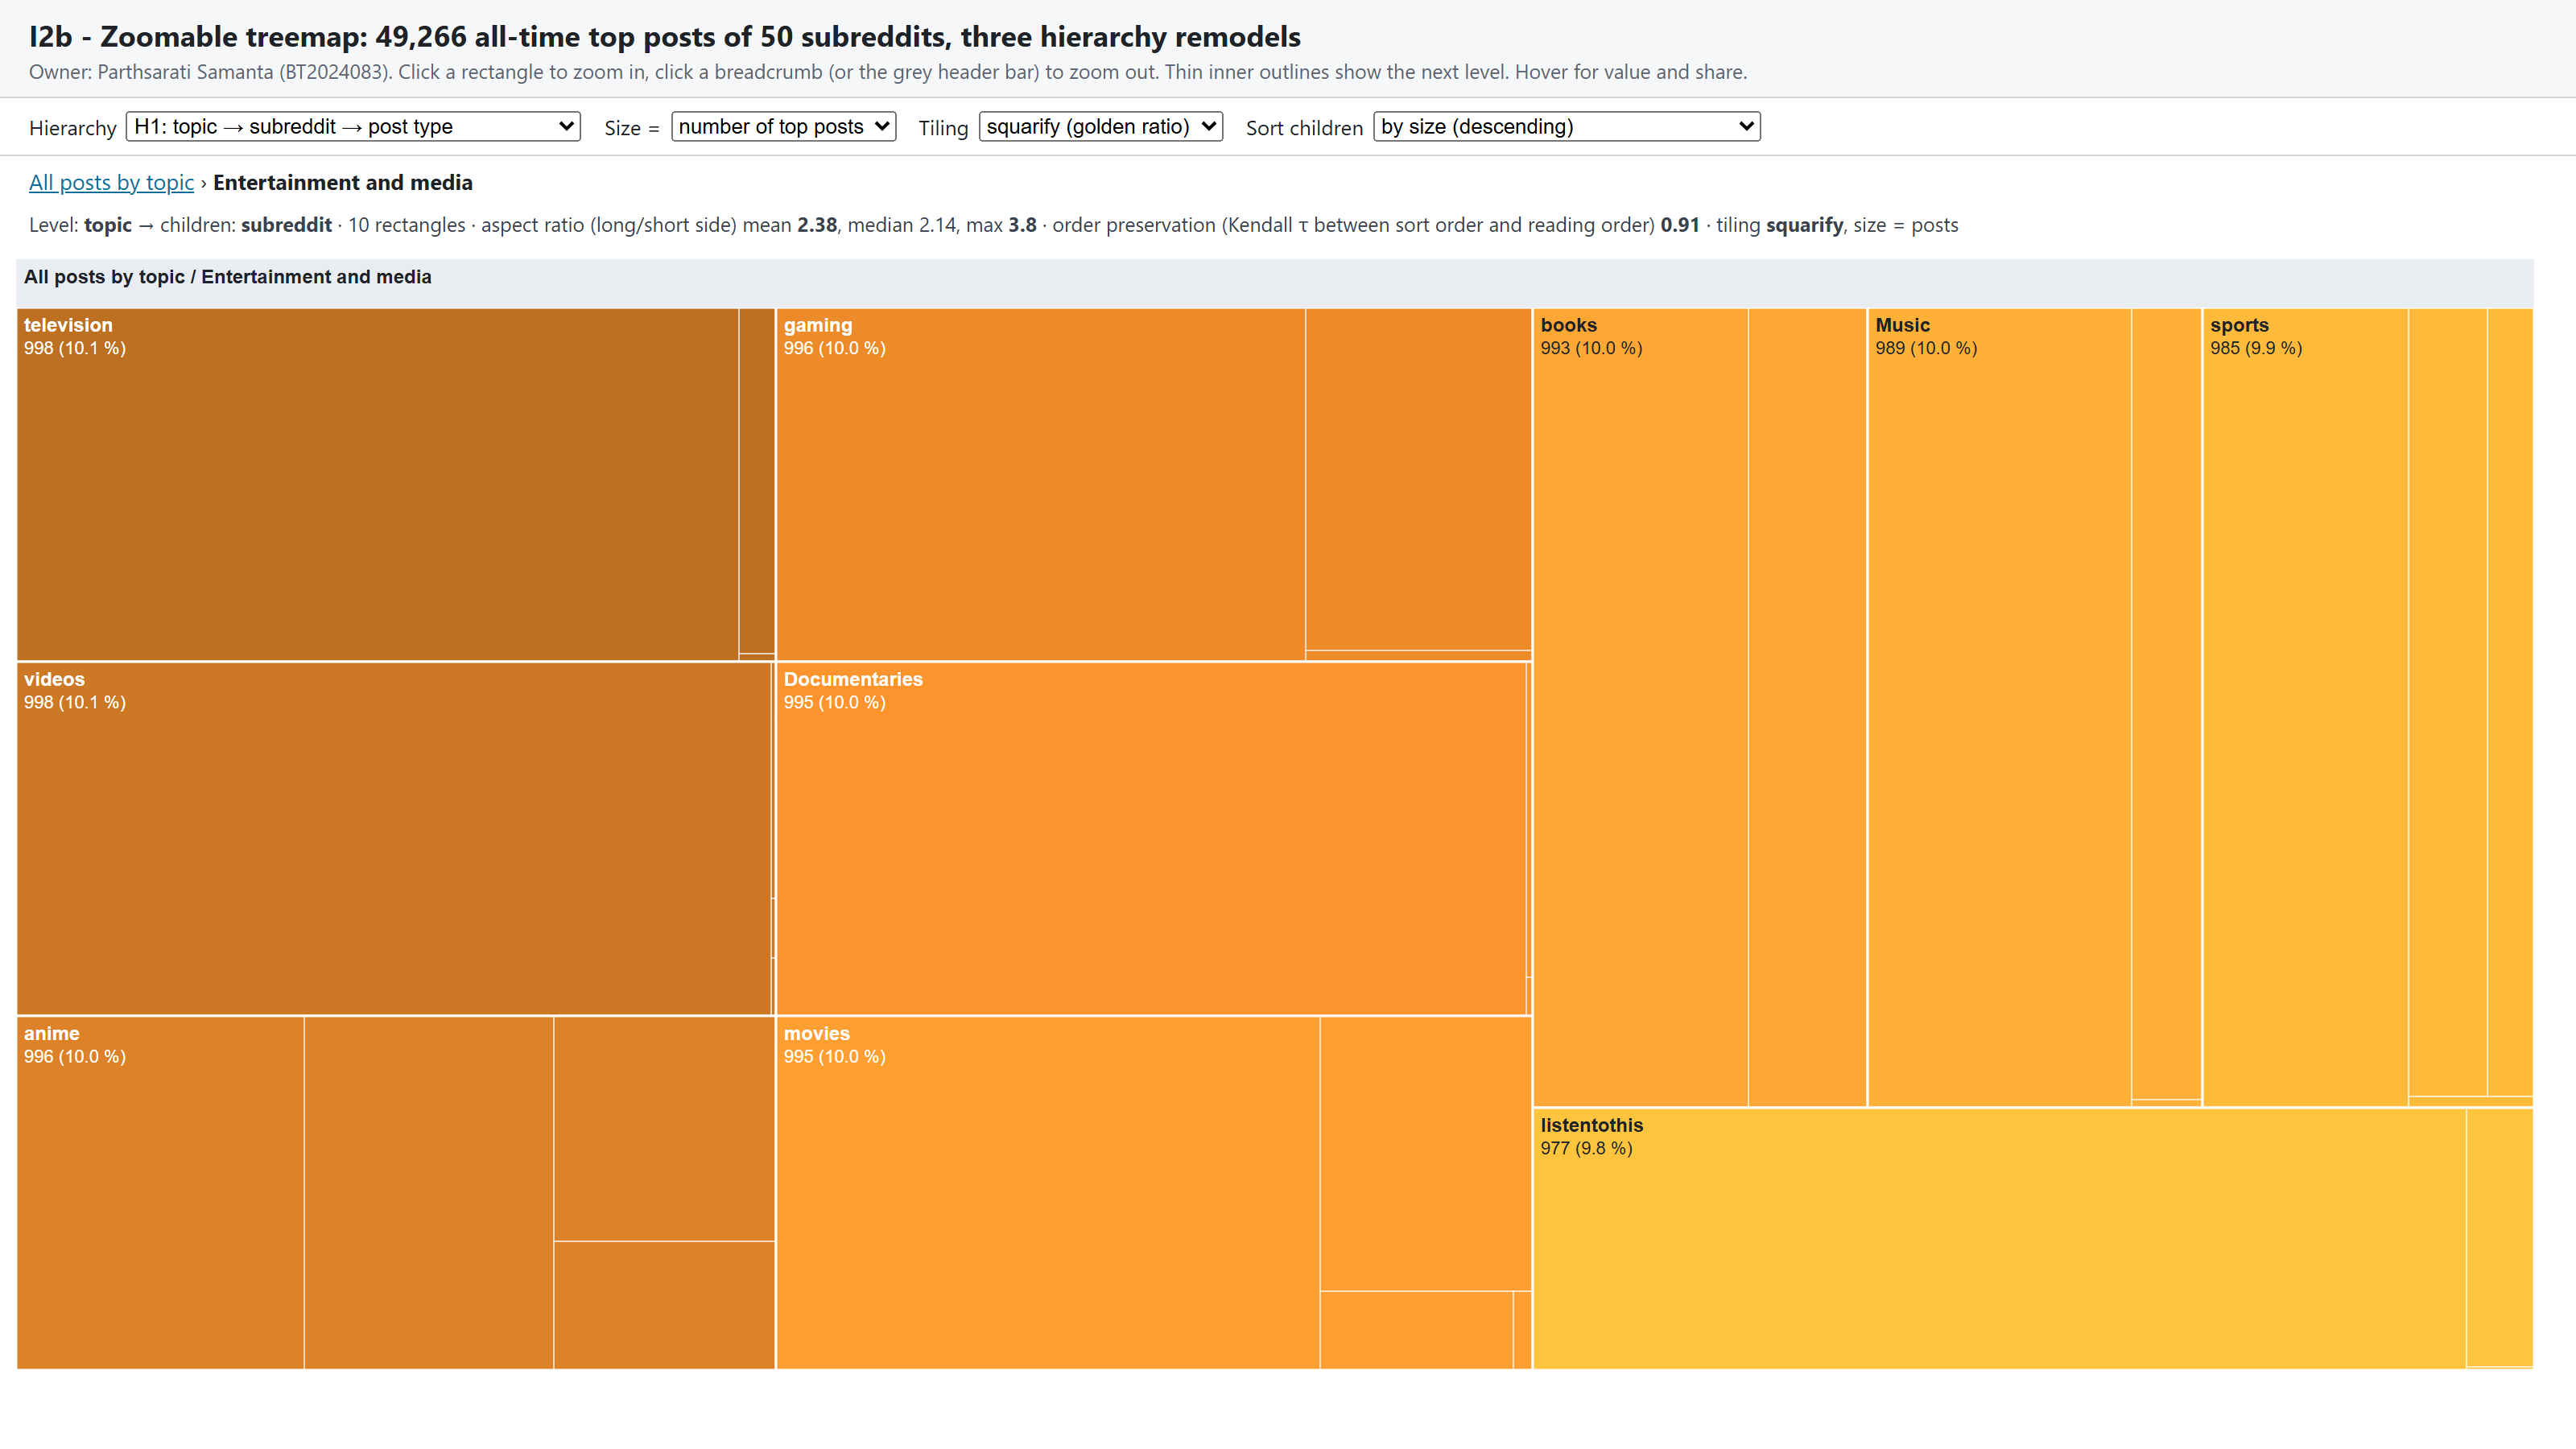
\includegraphics[width=0.495\textwidth]{Fig_33d_treemap_zoom_entertainment.png}}\\
\subfloat[H3 zoomed to 2019--20 / 2020, size = comments, sorted by name]{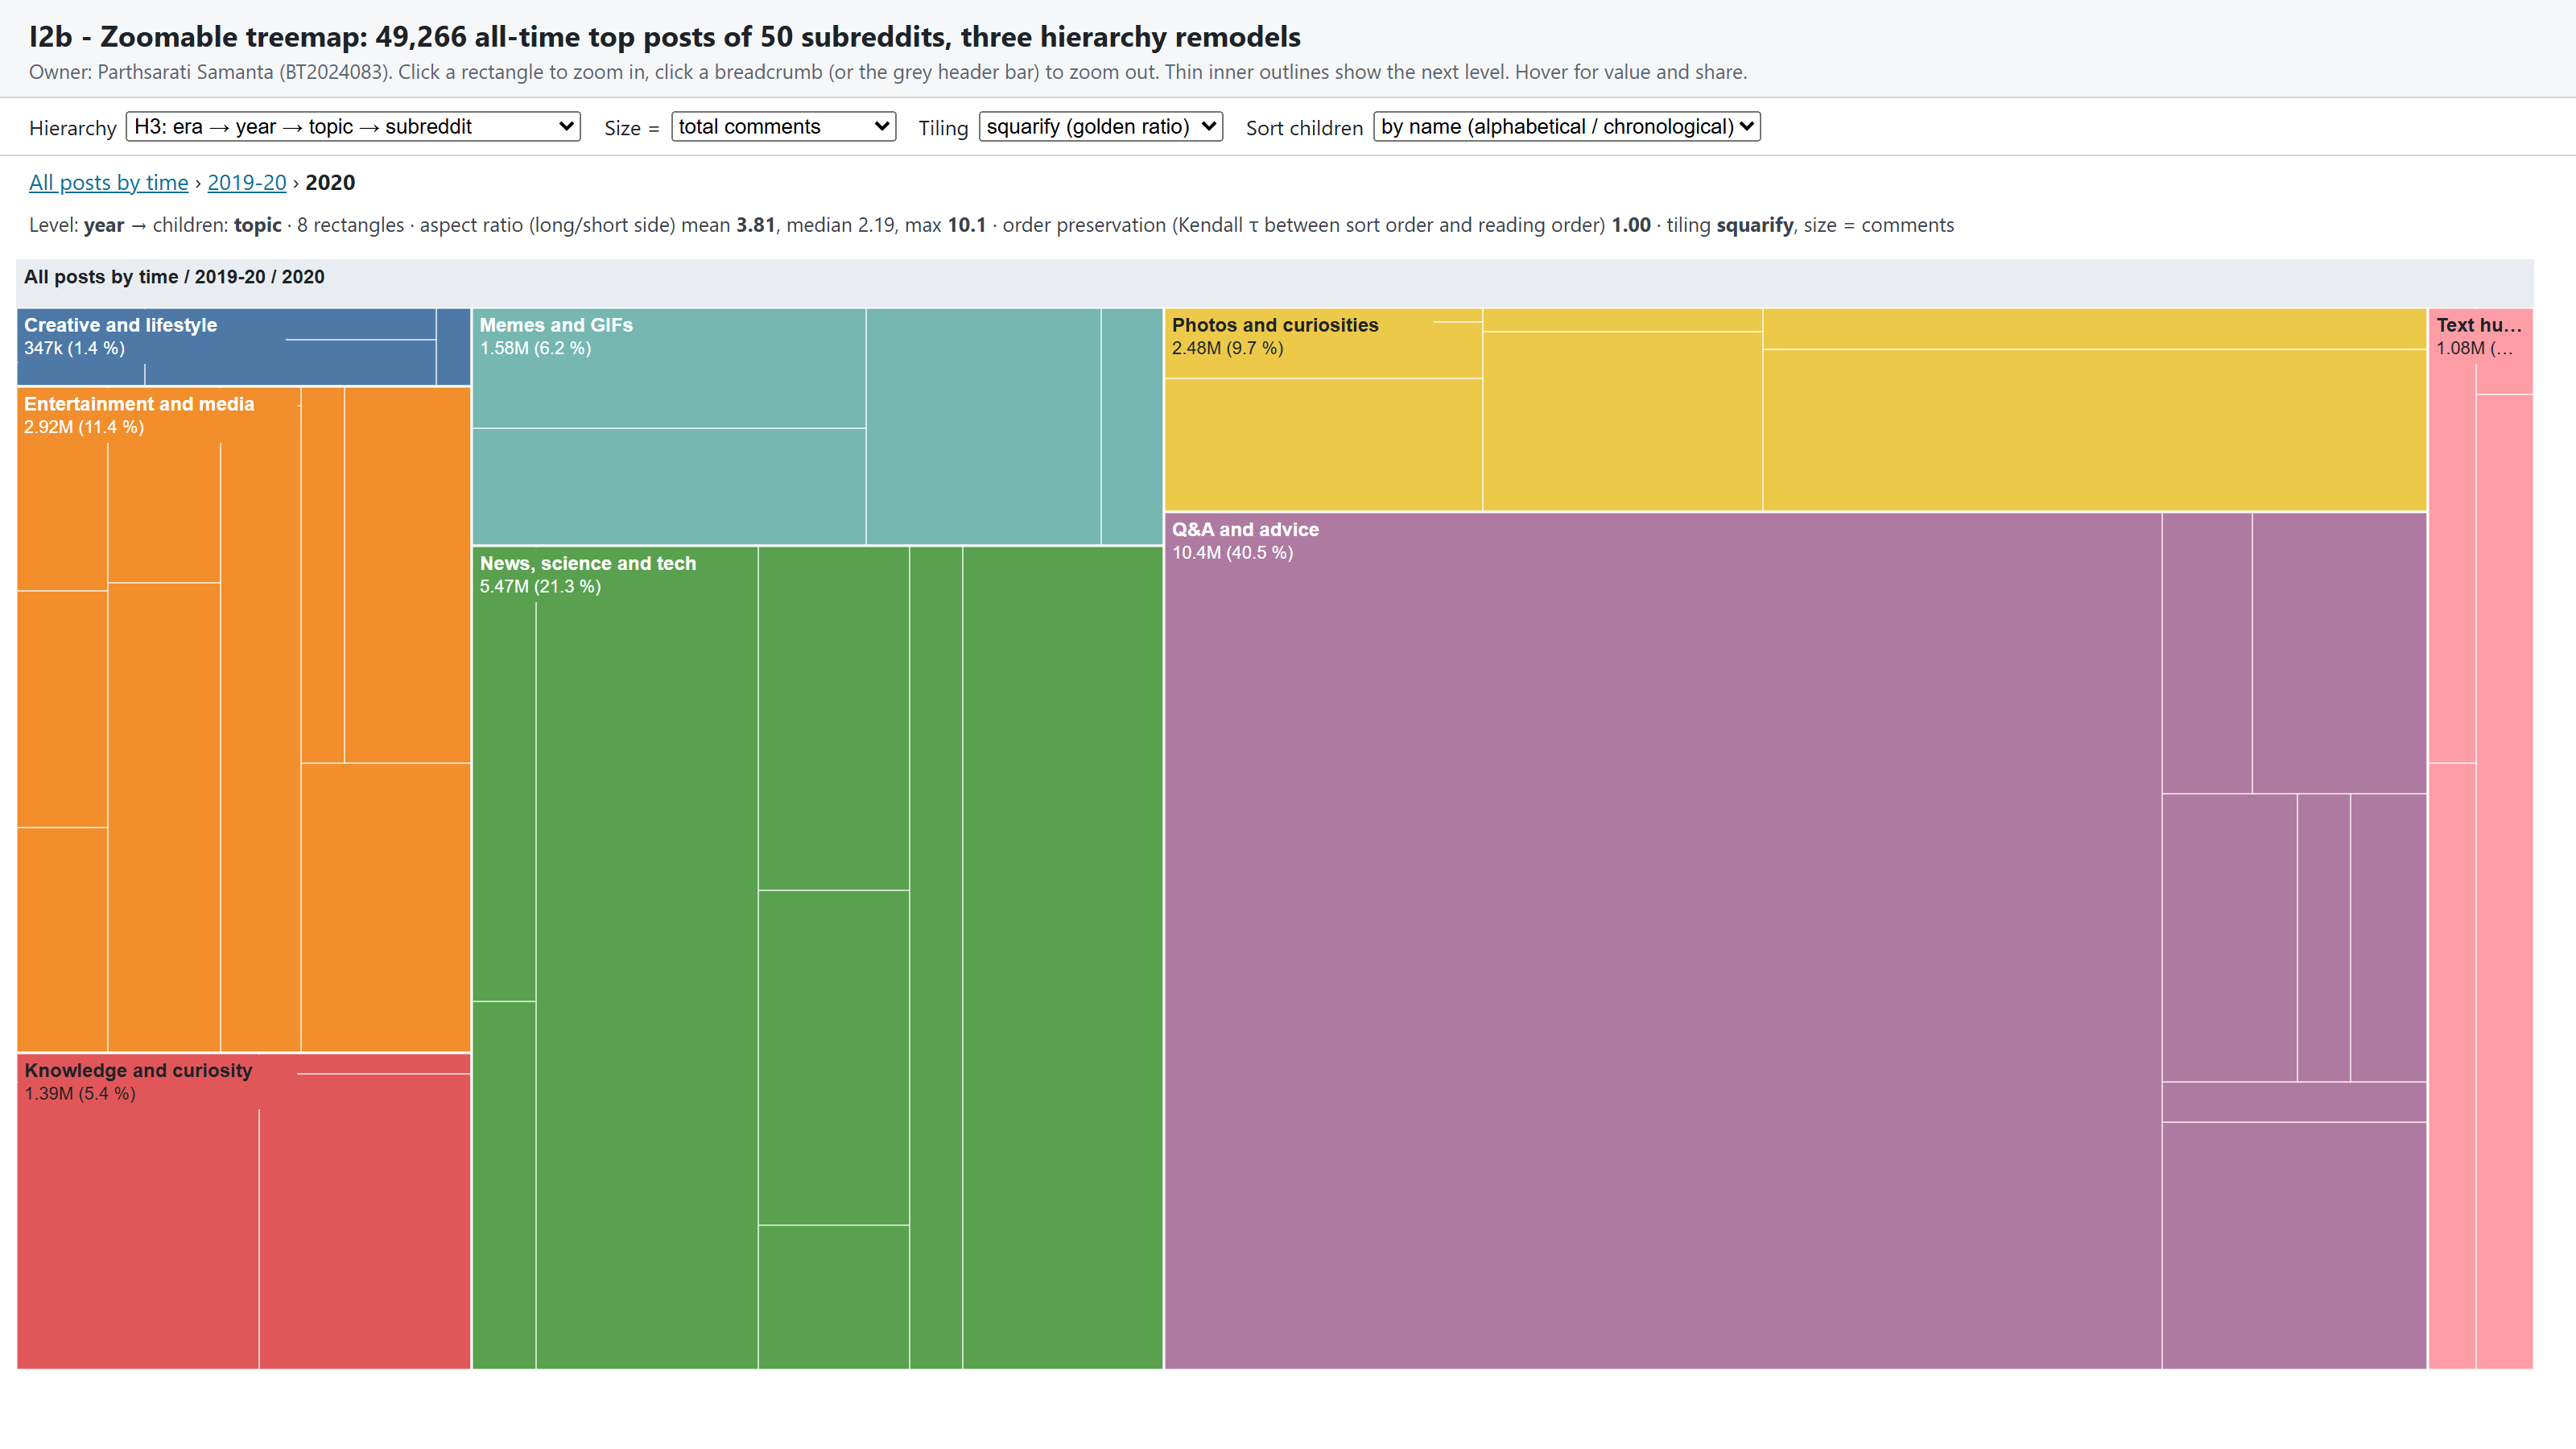
\includegraphics[width=0.495\textwidth]{Fig_33e_treemap_zoom_2020_comments.png}}\hfill
\subfloat[H2 zoomed into link posts, size = total score]{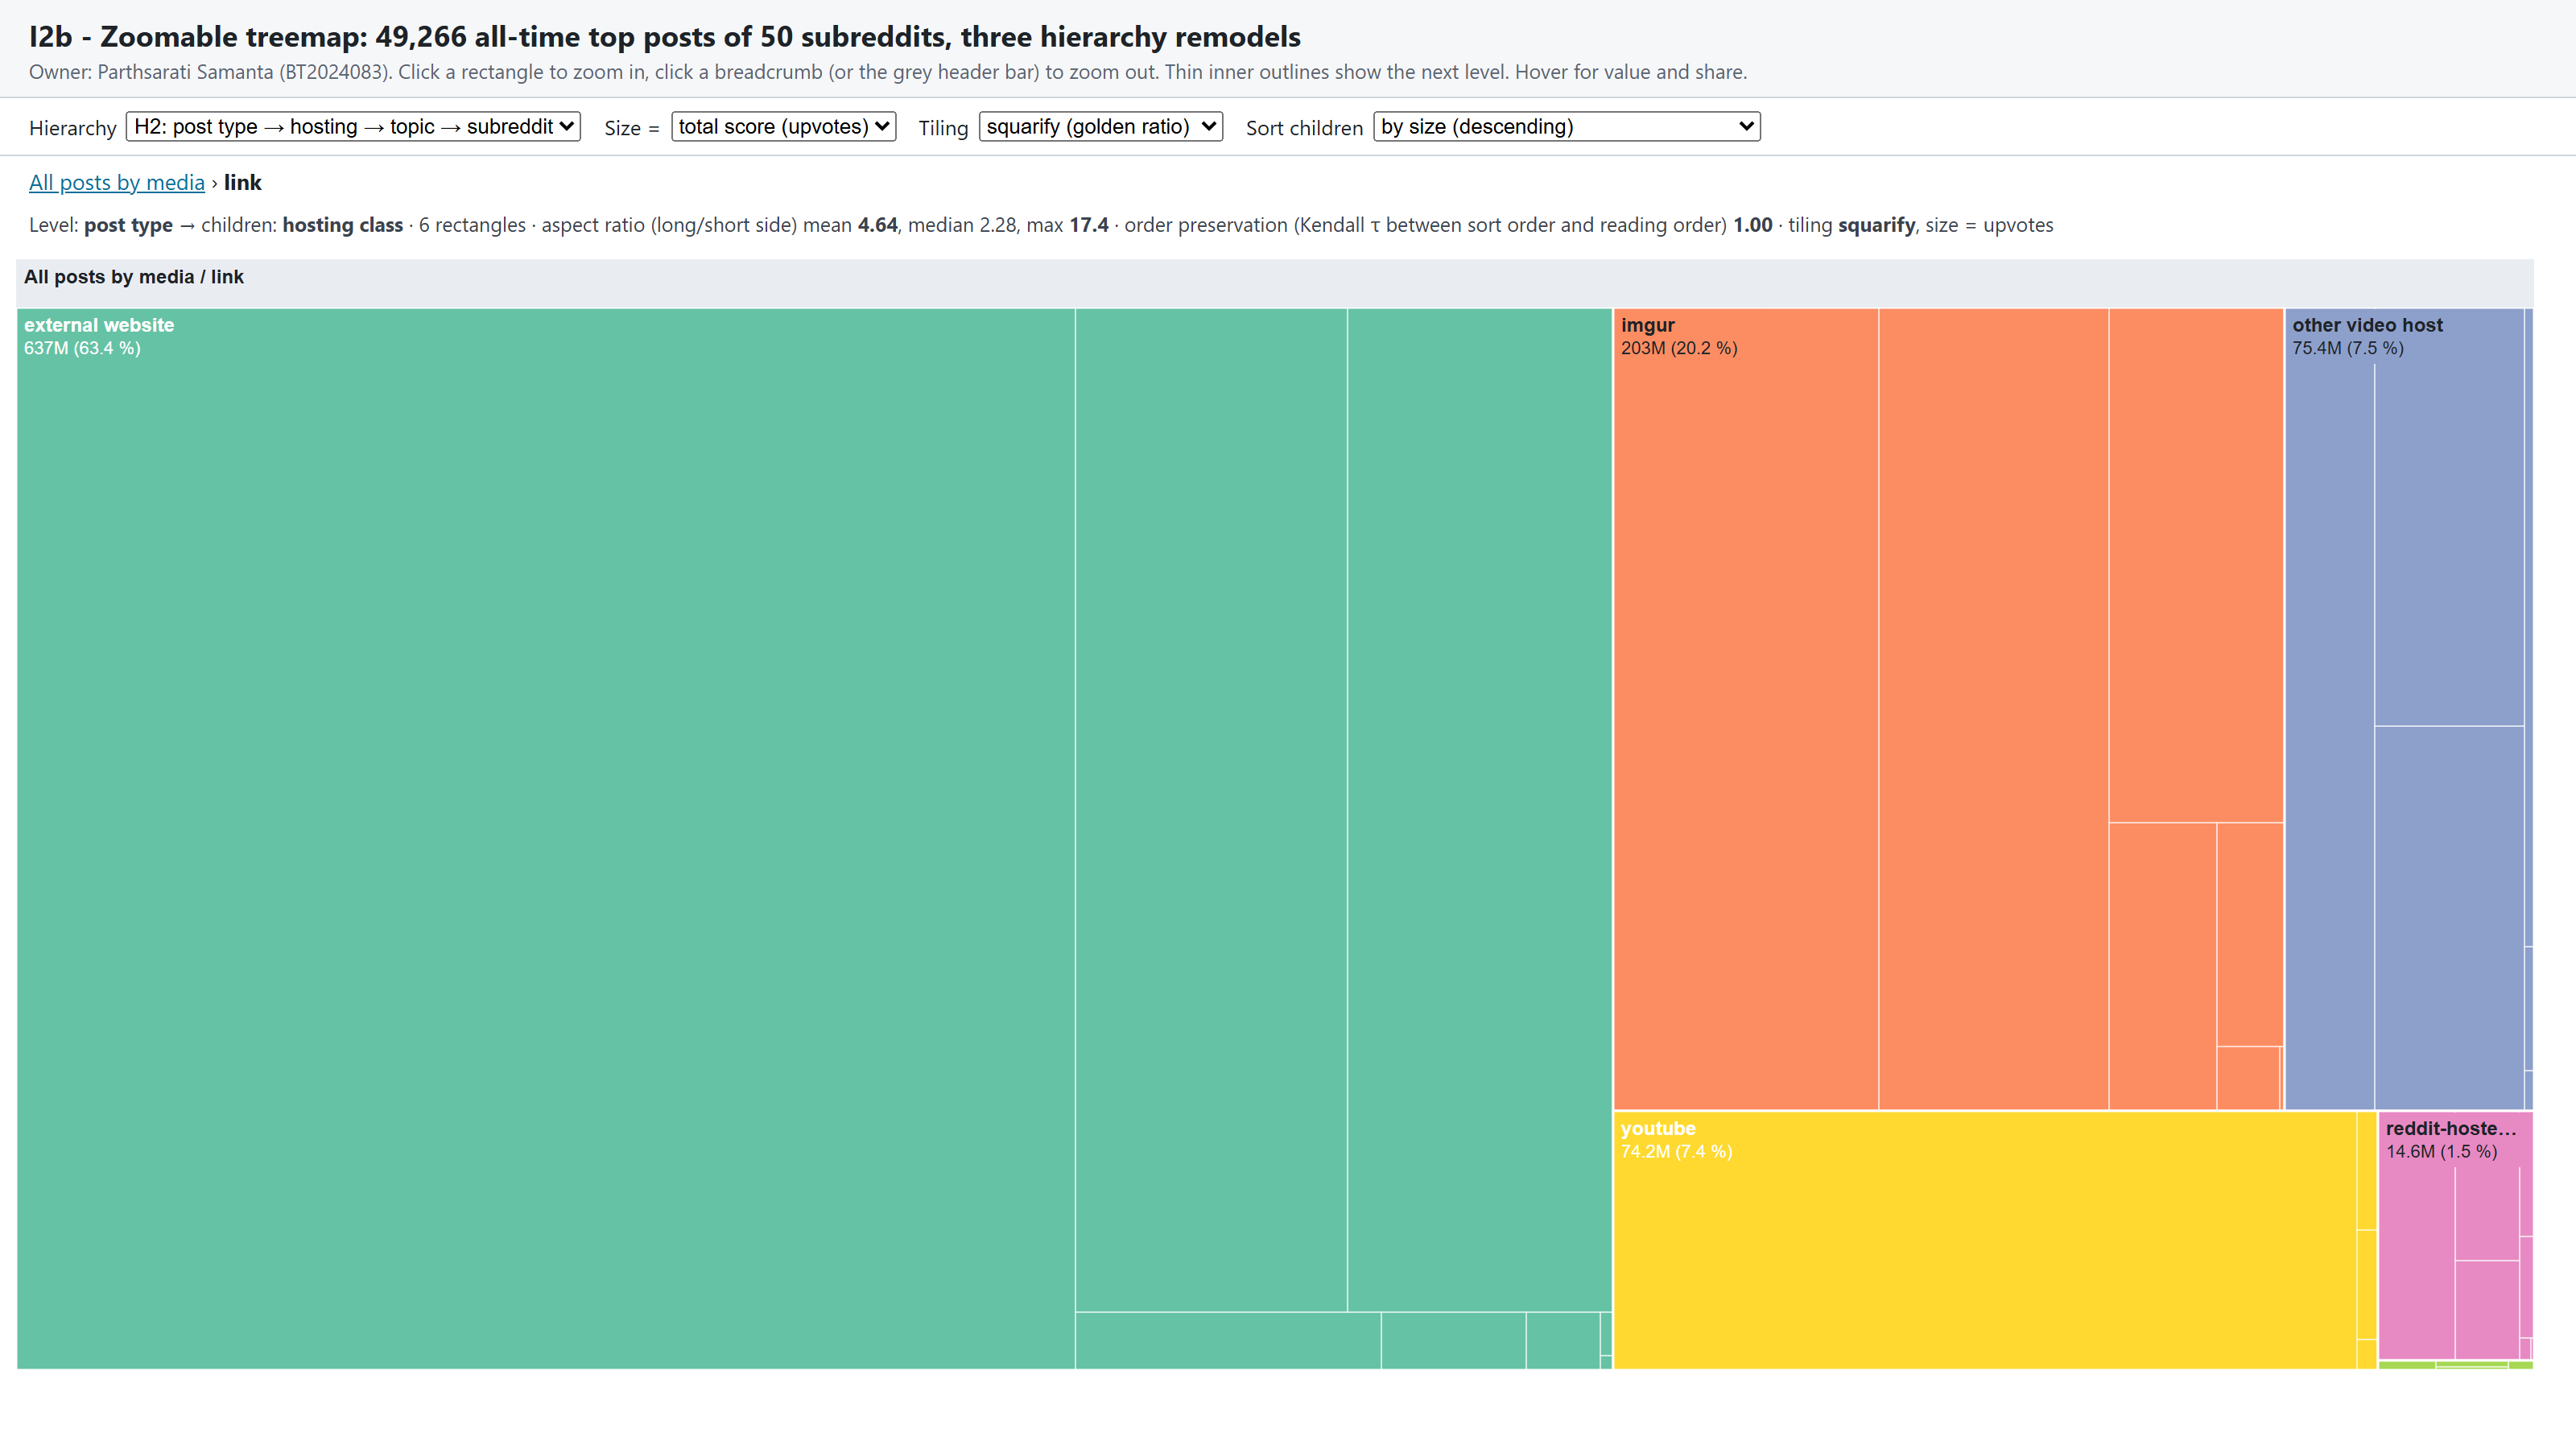
\includegraphics[width=0.495\textwidth]{Fig_33f_treemap_zoom_link_score.png}}
\caption{Zoomable treemap: three hierarchy remodels of the same 49,266 posts (a--c) and three zoom states (d--f), all with
squarify tiling. Files \fpath{Fig_33a..f_*.png}.}
\label{fig:33}
\end{figure*}

\textbf{Inferences (remodels and zoom, Fig.~\ref{fig:33}).}
(1) \textbf{H1 by posts} (Fig.~\ref{fig:33}a) is nearly uninformative at the subreddit level, because the dataset samples
about 1,000 posts per subreddit. Topic areas are proportional to how many subreddits each topic has, e.g.\
Entertainment 20.1\,\% with 10 subreddits. Zooming into Entertainment (Fig.~\ref{fig:33}d) confirms ten rectangles of
9.8--10.1\,\% each. The treemap thus exposes a \emph{sampling artefact}, and the measure must be changed before it can
answer a question about popularity.
(2) Switching the measure answers different questions. By \emph{total score}, Photos and curiosities lead with 22.6\,\%,
followed by News (18.8\,\%) and Memes (18.3\,\%), while Q\&A drops to 8.8\,\%. By \emph{total comments}, Q\&A leads with
29.6\,\% and News has 23.6\,\%, while Memes shrink to 6.0\,\%. Visual communities win upvotes and discussion communities
win comments, which repeats the A1 finding in a different visual form.
(3) \textbf{H2} (Fig.~\ref{fig:33}b) shows that links are the largest post type (41.0\,\%), followed by images (28.2\,\%),
text (26.6\,\%) and video (4.2\,\%). Zooming into links weighted by score (Fig.~\ref{fig:33}f) shows that external websites
take 63.4\,\% of link upvotes, imgur 20.2\,\%, other video hosts 7.5\,\% and YouTube 7.4\,\%. Text posts are always self
posts by definition, so H2's hosting level is degenerate for them, which is itself a validation of the classification.
(4) \textbf{H3} (Fig.~\ref{fig:33}c) shows the temporal skew of the corpus: 2019--20 holds 40.5\,\% of the posts, 2017--18
29.2\,\%, 2021--22 20.7\,\%, and the oldest and newest eras only 5.1\,\% and 4.5\,\%. Zooming to 2020 sized by comments
(Fig.~\ref{fig:33}e) shows that Q\&A alone produced 40.5\,\% of 2020's comments (10.4\,M), twice its post share. This is
consistent with heavy discussion during the 2020 lockdowns.
(5) Comparing remodels shows that the first level of the hierarchy decides what can be compared directly. Topics are
adjacent in H1, media types in H2 and time in H3. The same subreddit appears as one rectangle in H1 but is split
across four post types in H2 and across up to 14 years in H3.

\begin{figure*}[!t]
\centering
\subfloat[squarify]{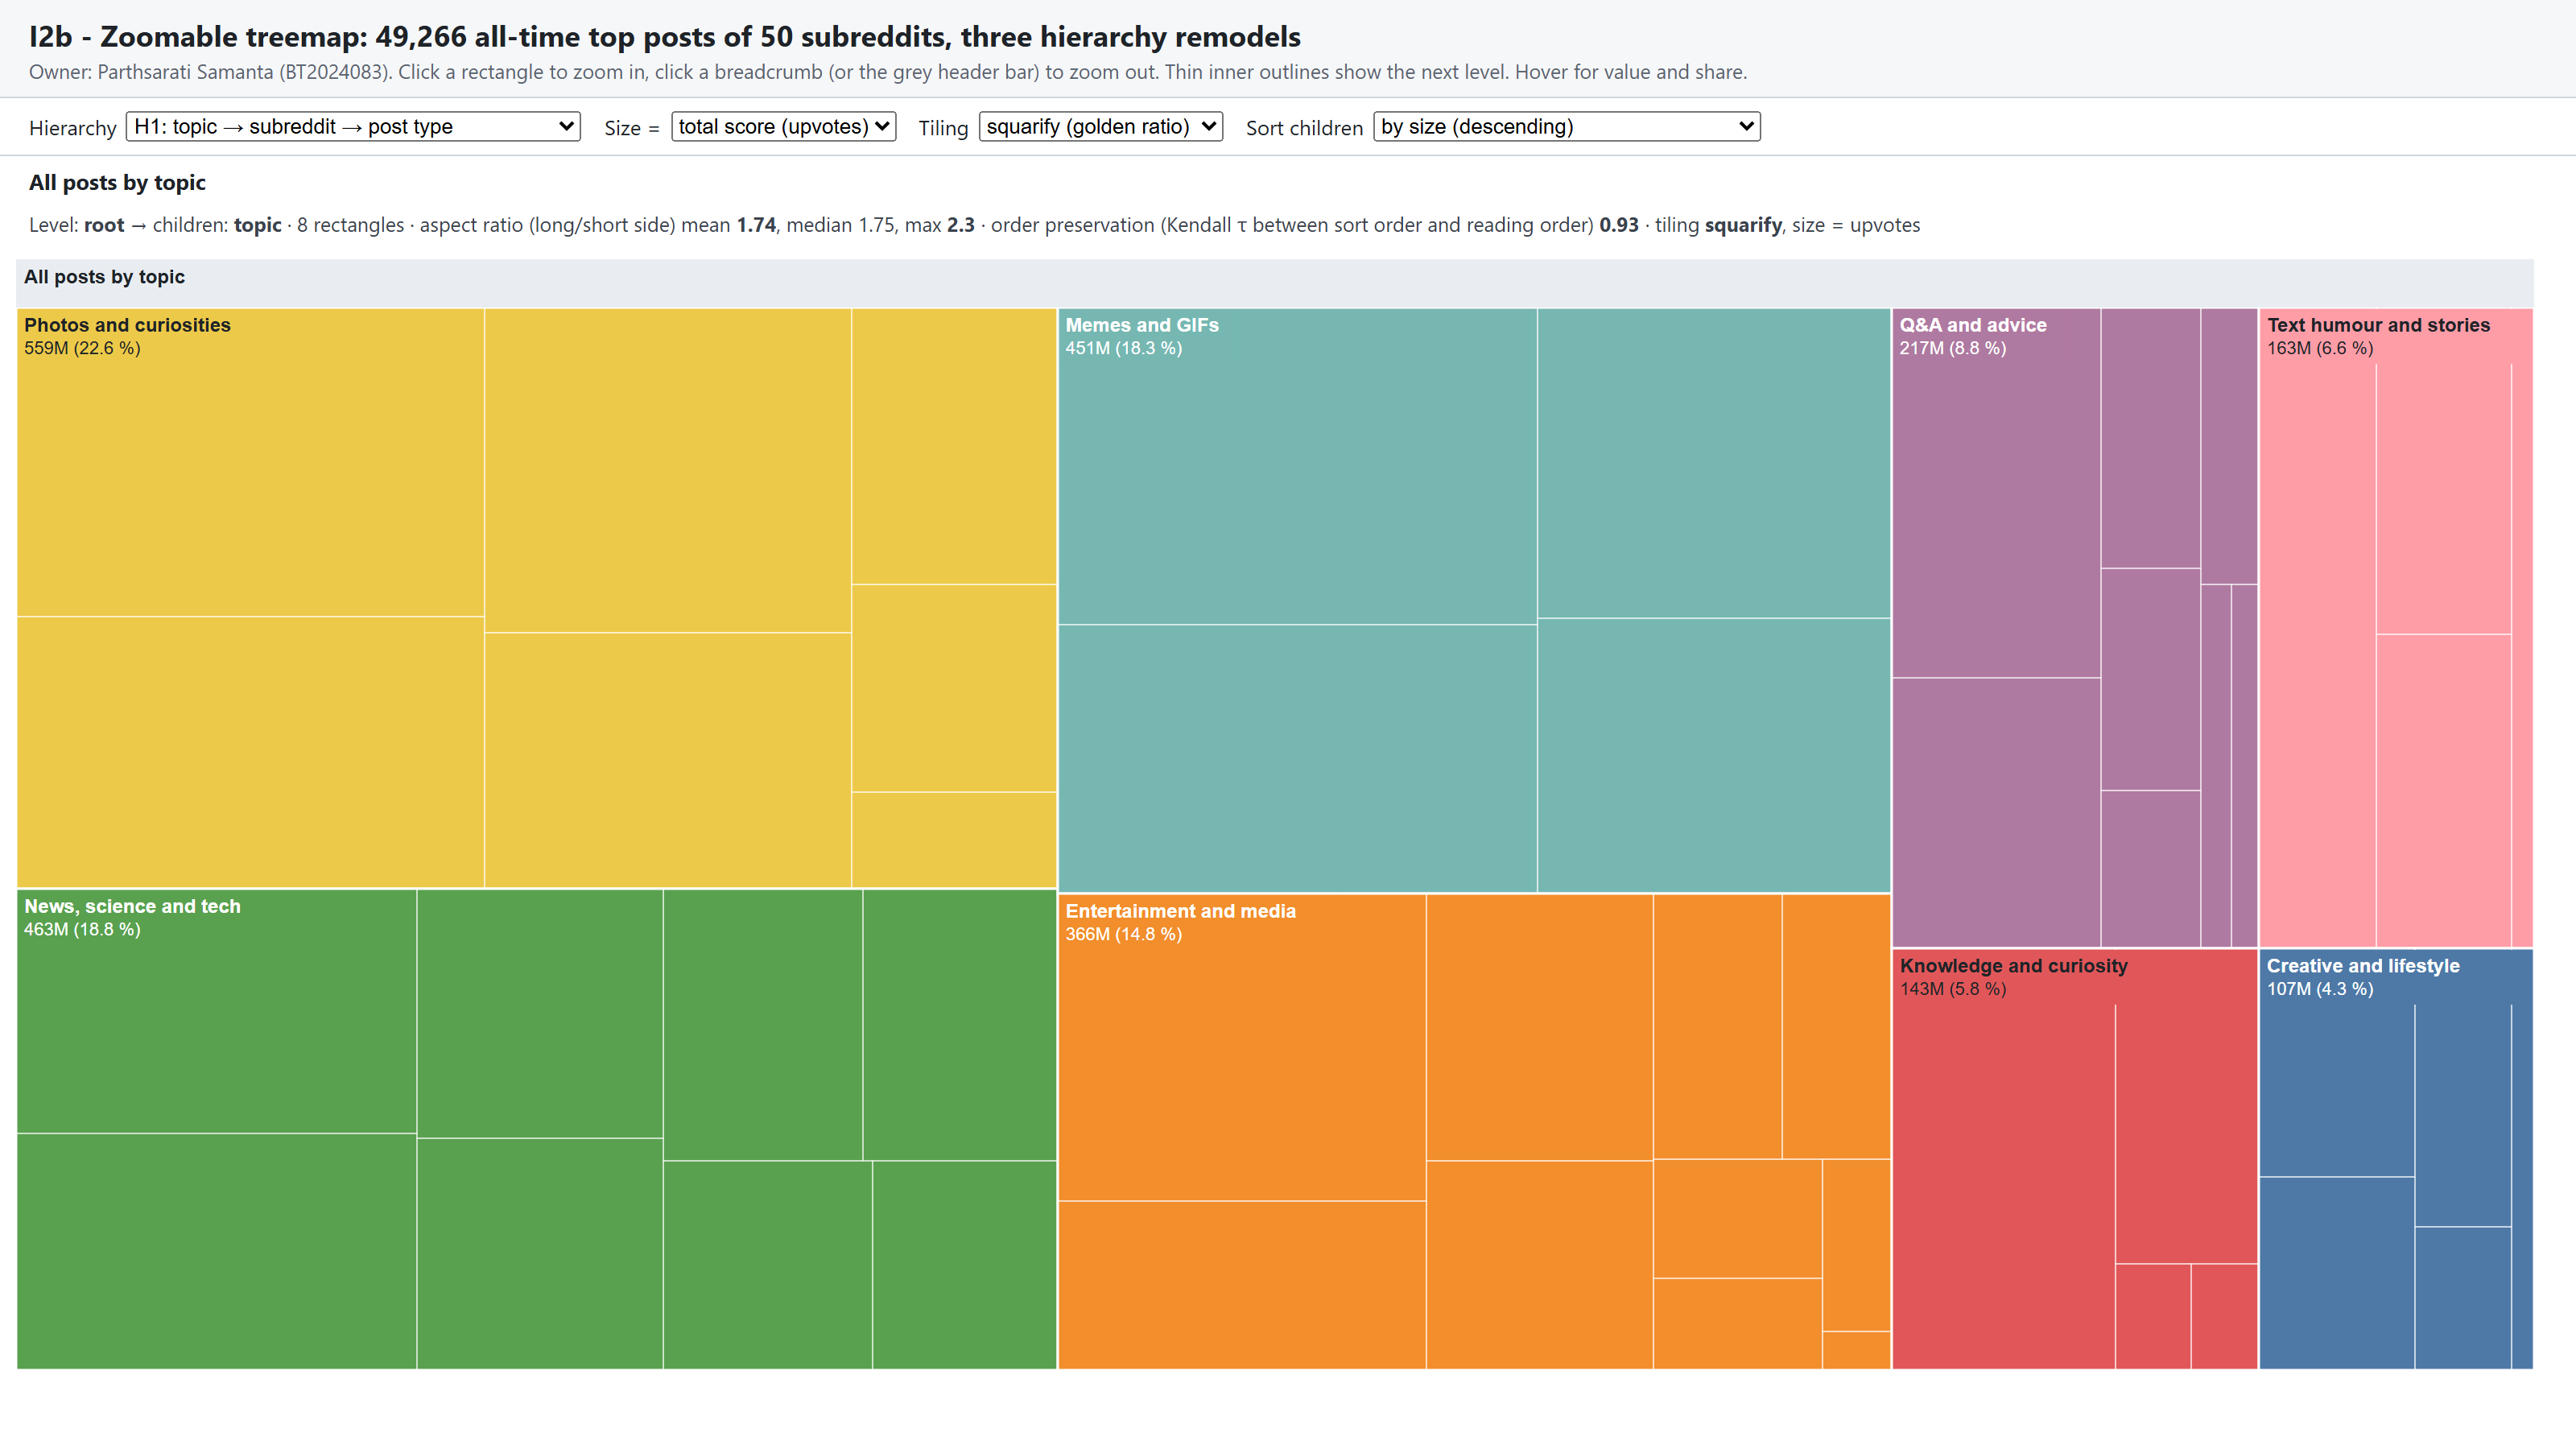
\includegraphics[width=0.33\textwidth]{Fig_34a_treemap_tiling_squarify.png}}\hfill
\subfloat[binary]{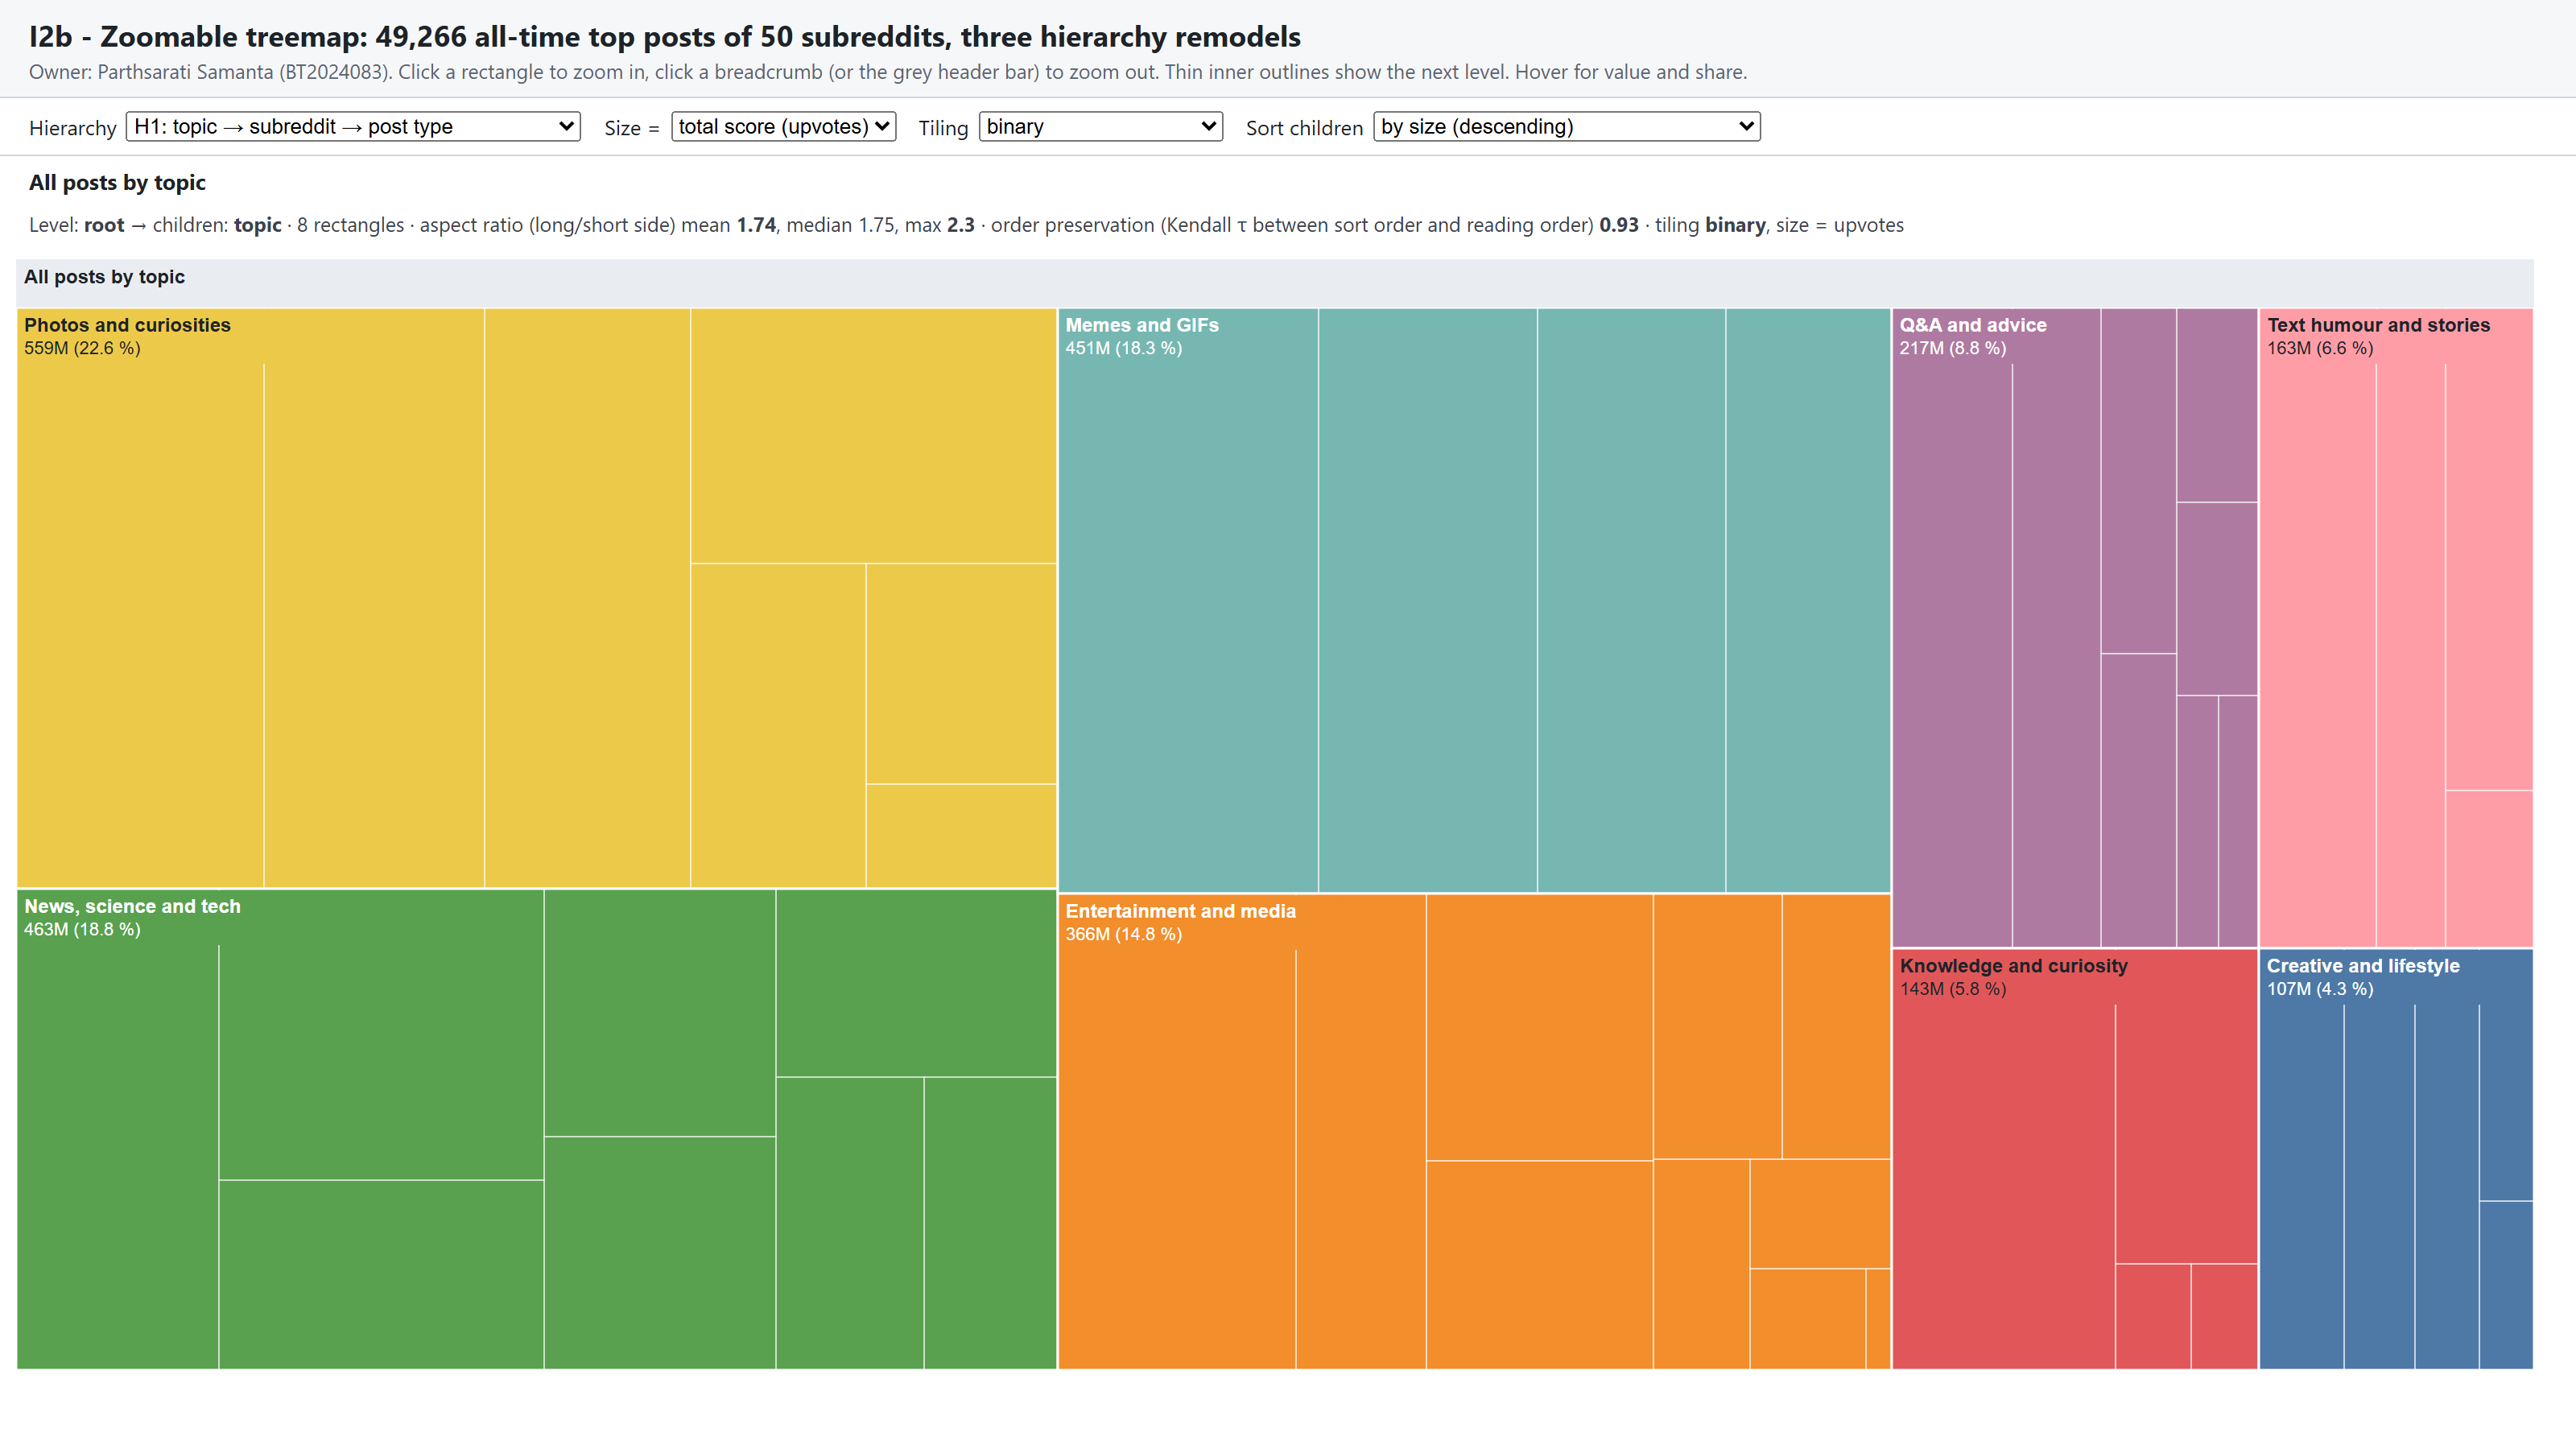
\includegraphics[width=0.33\textwidth]{Fig_34b_treemap_tiling_binary.png}}\hfill
\subfloat[slice]{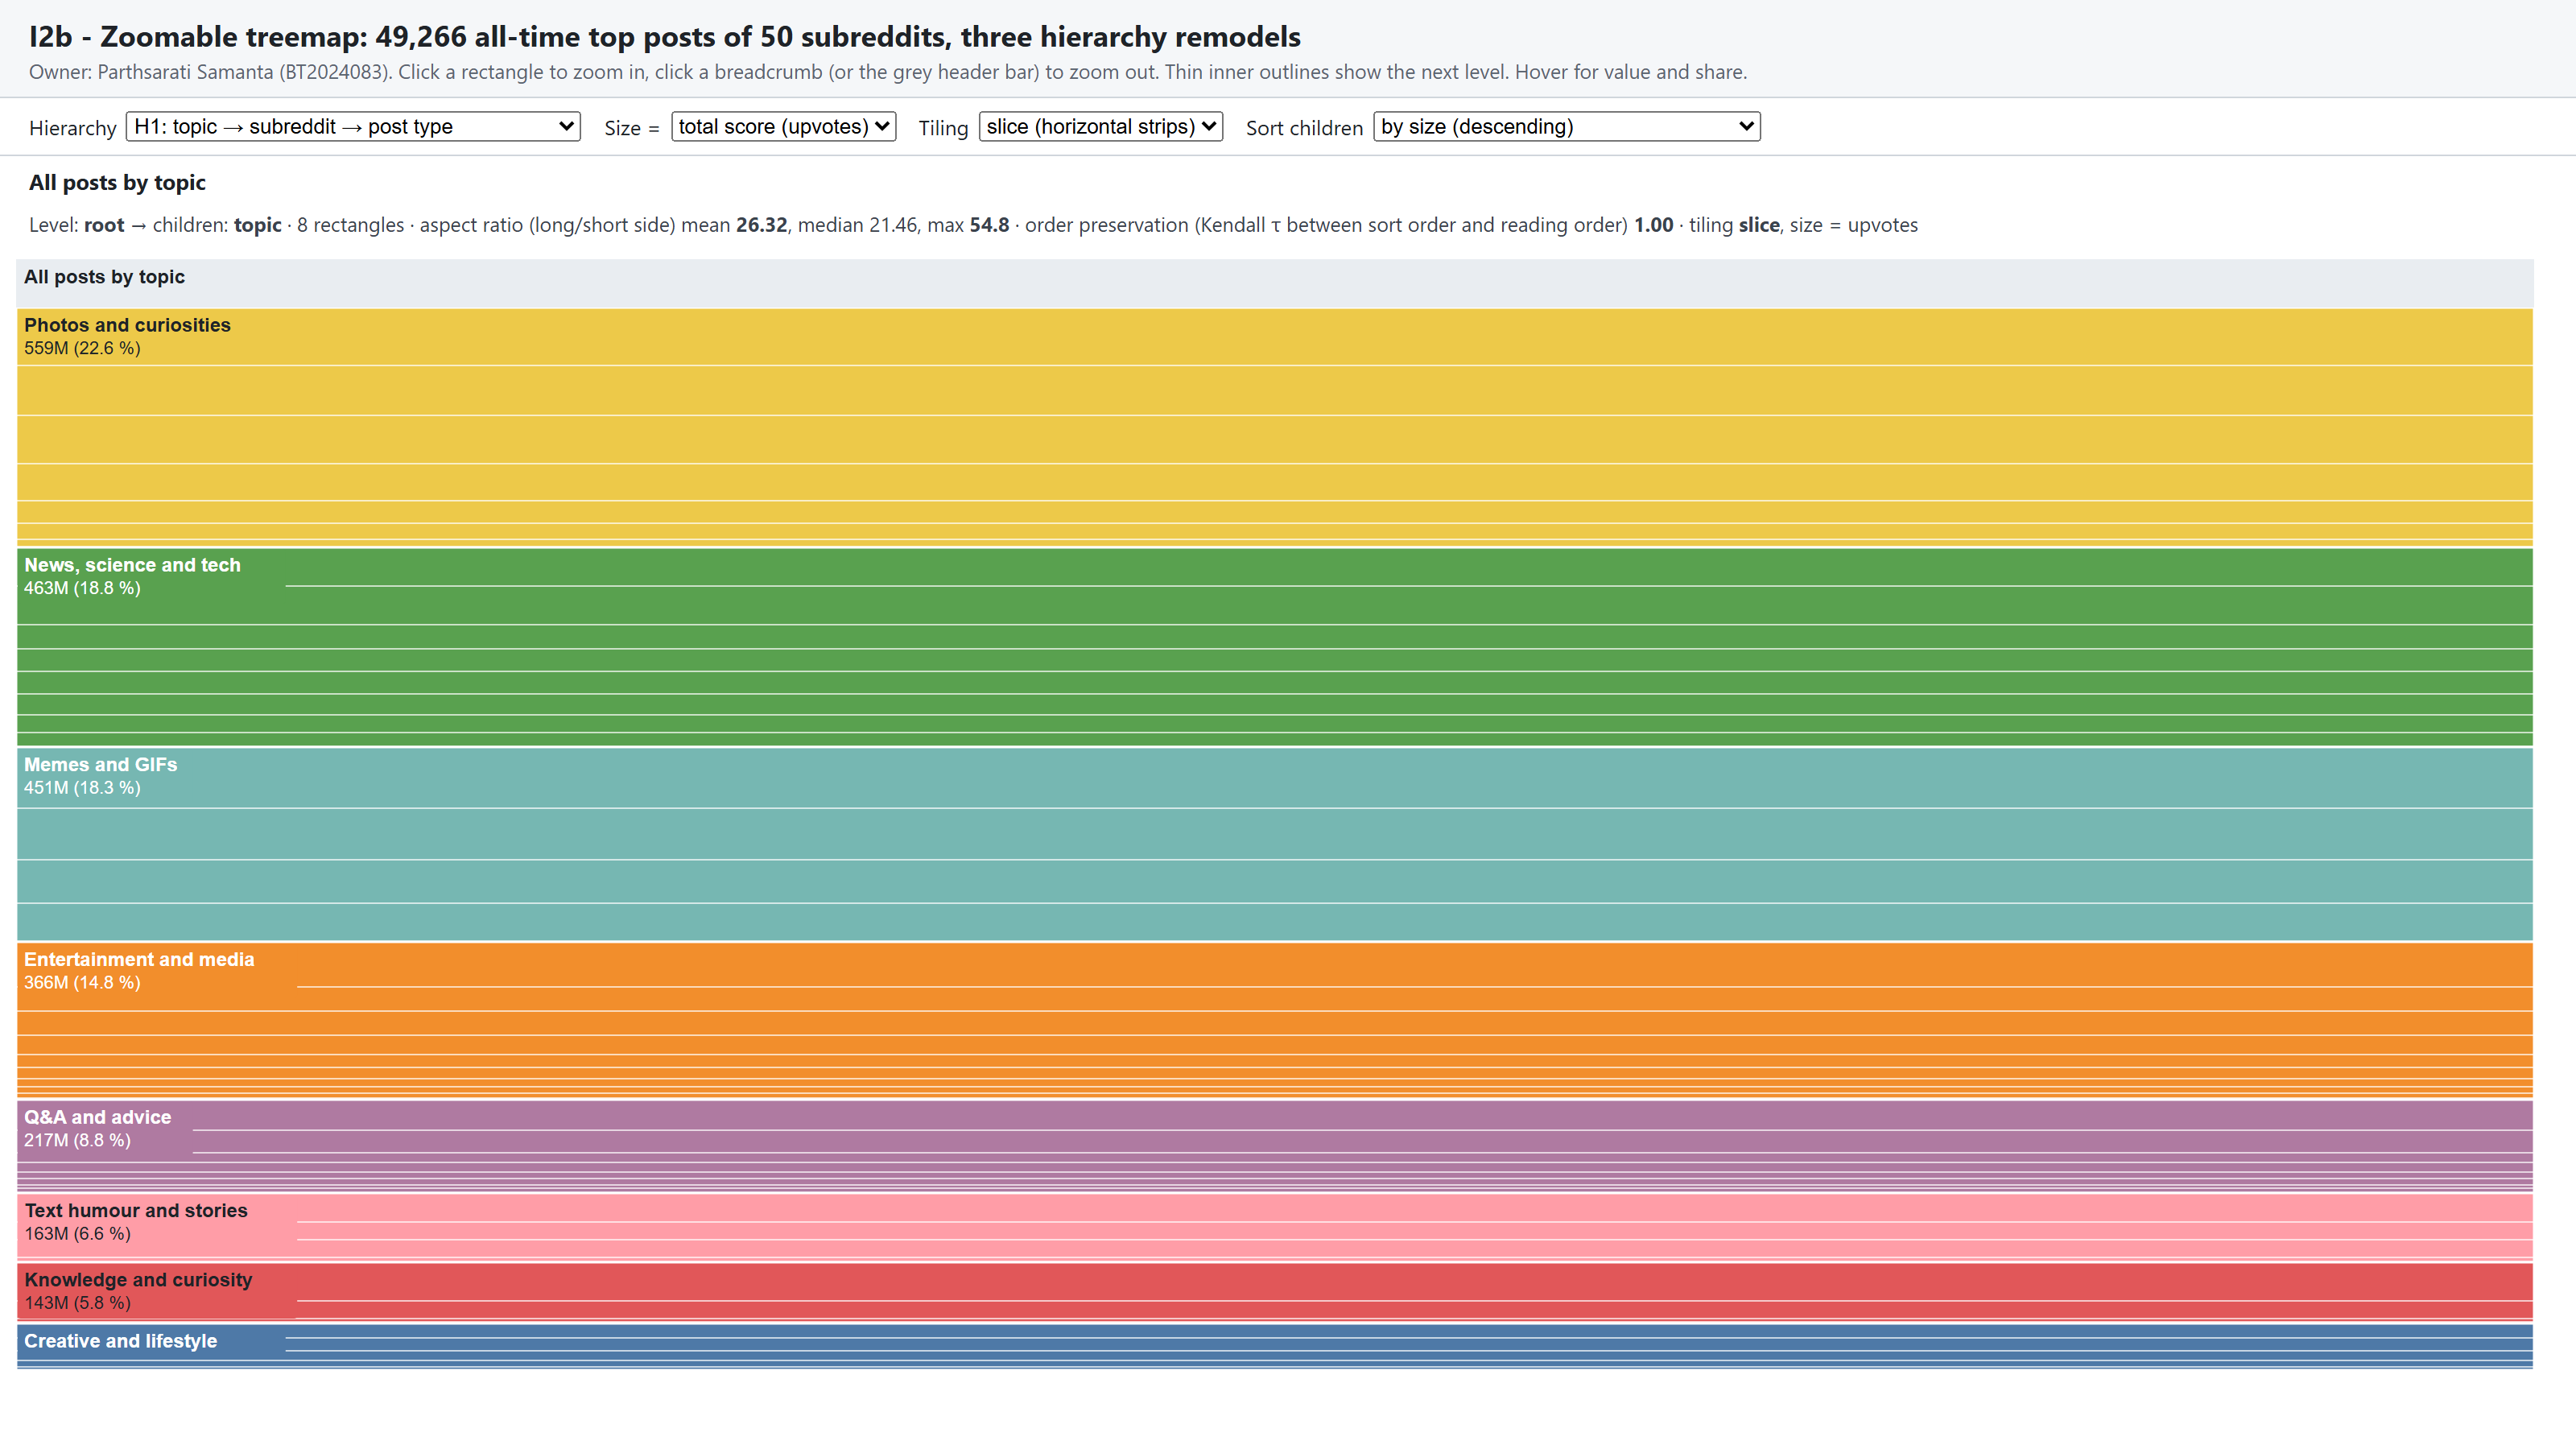
\includegraphics[width=0.33\textwidth]{Fig_34c_treemap_tiling_slice.png}}\\
\subfloat[dice]{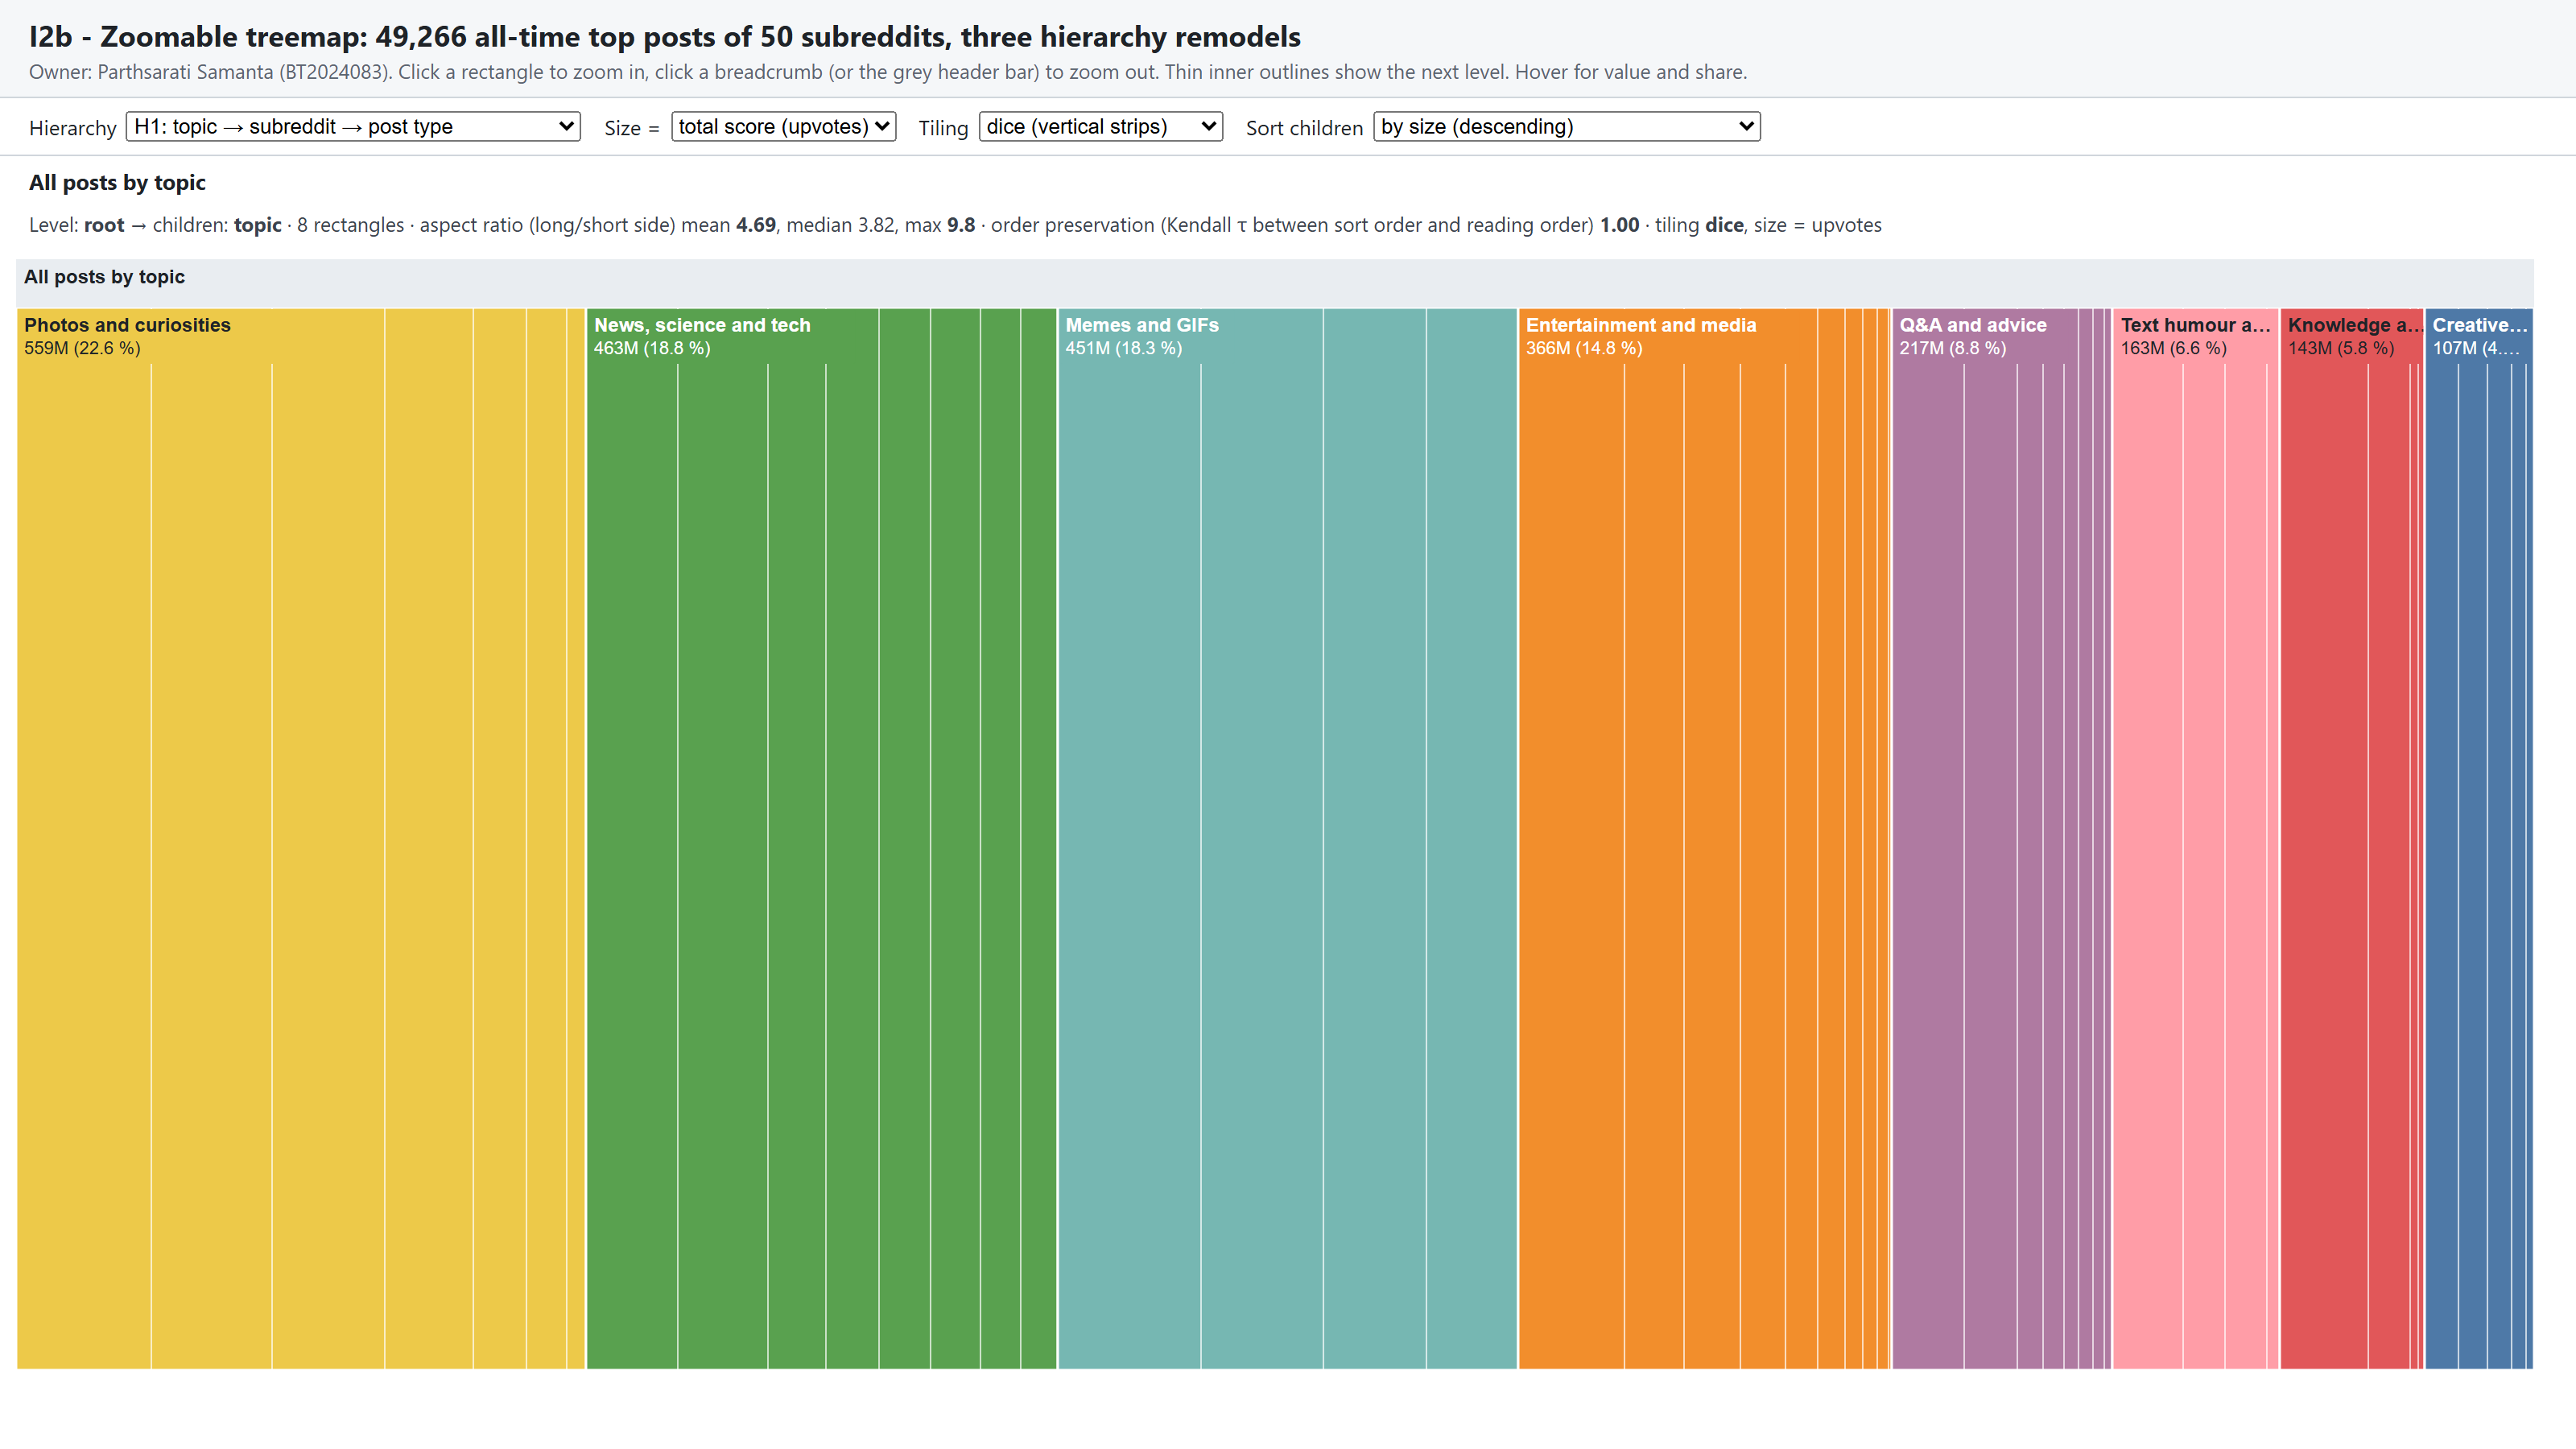
\includegraphics[width=0.33\textwidth]{Fig_34d_treemap_tiling_dice.png}}\hspace{0.02\textwidth}
\subfloat[slice-dice]{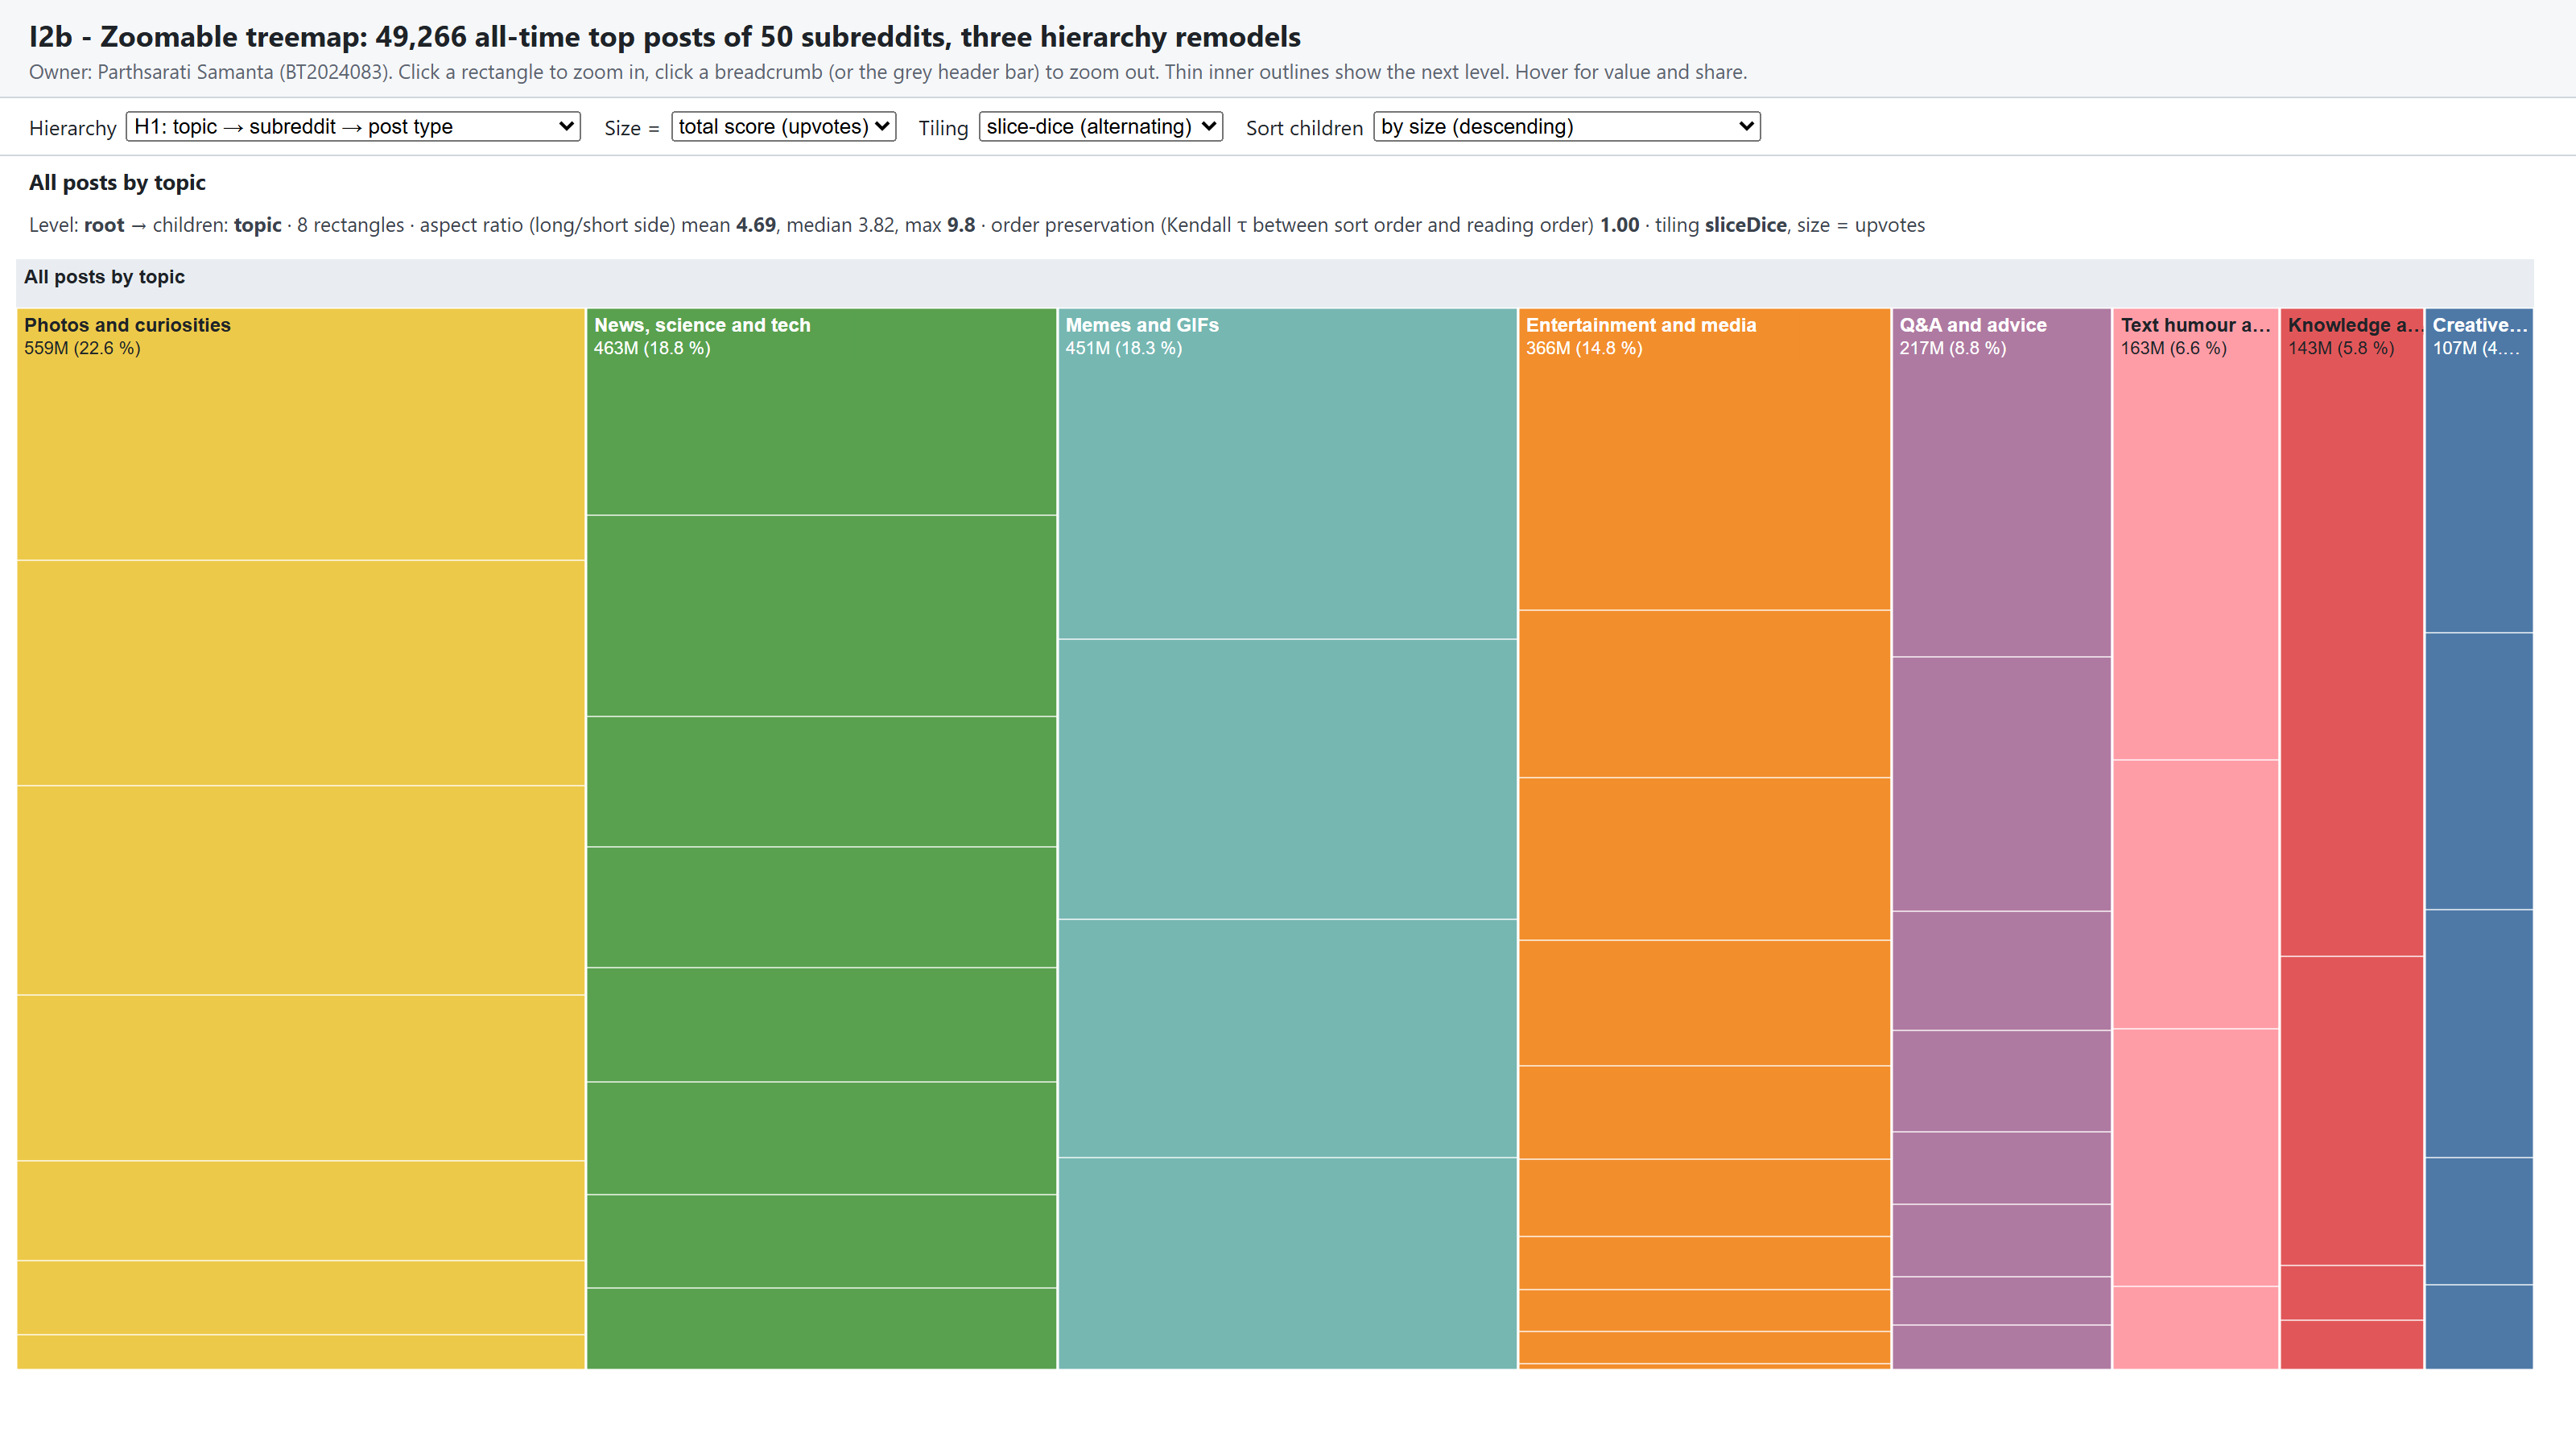
\includegraphics[width=0.33\textwidth]{Fig_34e_treemap_tiling_sliceDice.png}}
\caption{The five tiling strategies on the same view (H1 root, size = total score, children sorted by size). Files
\fpath{Fig_34a..e_*.png}.}
\label{fig:34}
\end{figure*}
\input{generated/tab_tiling}

\textbf{Inferences (tiling, Fig.~\ref{fig:34}, Table~\ref{tab:tiling}).}
(1) Squarify and binary give near-square rectangles (mean aspect ratio 1.6--2.2), which makes areas easy to compare and
leaves room for labels. Their worst cases (5.4--10.0) all occur in the H2 root, where the video category holds only
4\,\% of posts and must become a strip. Binary is the most balanced overall (mean 1.56 when sorted by size).
(2) Slice and dice keep the sort order perfectly ($\tau=1$) but produce extreme slivers: slice has a mean aspect ratio of
18.9 and a worst case of 56.3. In Fig.~\ref{fig:34}c the eight topics
become thin full-width strips. That is fine for ordered categories such as eras or years, but small items such as
Creative and lifestyle cannot be labelled.
(3) Slice-dice alternates direction by depth. It is good at the root (mean 3.8) but inherits slice's slivers one level
down (23.7 in the Entertainment view), and it preserves order.
(4) Squarify is the only tiling whose order preservation is below 1 ($\tau$ = 0.95--0.97). Its greedy rows place items out
of reading order, so ``what is next to what'' carries no meaning. Binary keeps $\tau\approx1$ with good aspect ratios.
For the chronological H3 hierarchy sorted by name, binary or slice-dice are therefore preferable, while squarify is best
for comparing magnitudes.

\subsection{Observations and limitations (I2)}
Bundling makes cluster structure readable in a 2,000-line plot, brushing turns it into a query tool, and reordering exposes
pairwise relations; the bundled view should be confirmed in the unbundled one. The treemap's value depends on choosing the
hierarchy and the measure deliberately; it also revealed the per-subreddit sampling design. Limitations: the
parallel-coordinates sample is 4\,\% of the corpus, and SVG rendering becomes sluggish beyond about 5,000 lines (canvas
would be needed). Treemaps cannot show negative or non-additive measures such as medians.

% ============================================================================================
\section{I3: Horizon and Ridgeline Plots (Owner: Shrey Modi, BT2024125)}
\label{sec:i3}
Both techniques are implemented by hand in Matplotlib (\fpath{infovis/i3_horizon_ridgeline/run.py}); no horizon or ridgeline
library is used.

\subsection{Horizon plot construction}
Horizon graphs~\cite{saito2005,heer2009} fold a time series into a compact band:
\begin{enumerate}
\item centre the series on a baseline $b$ (the row's mean or median): $d_t=x_t-b$;
\item choose $N$ bands of height $h=\max|d|/N$, shared by all rows of a figure so that rows are comparable;
\item slice the positive part into bands $p_t^{(k)}=\mathrm{clip}(d_t-kh,0,h)$ and the negative part into
  $n_t^{(k)}=\mathrm{clip}(-d_t-kh,0,h)$, for $k=0..N{-}1$;
\item \emph{fold} the negative bands upward onto the same $[0,h]$ strip and overlay all bands, drawing band $k$ in the
  $k$-th saturation of a diverging palette (reds above the baseline, blues below; RdBu).
\end{enumerate}
Fig.~\ref{fig:35} shows each step on the monthly ``Q\&A and advice'' series and compares $N=1,2,3,4,6$.

\begin{algorithm}[!t]
\caption{Horizon band folding for one row}
\label{alg:horizon}
\begin{algorithmic}[1]
\REQUIRE series $x_{1..T}$, baseline $b$, band height $h$, bands $N$, palettes $C^+_{1..N}$, $C^-_{1..N}$
\STATE $d_t\leftarrow x_t-b$
\FOR{$k=0$ \TO $N-1$}
  \STATE $p_t\leftarrow\min(\max(d_t-kh,0),h)$; \ fill area $[0,p_t]$ with $C^+_{k+1}$
  \STATE $n_t\leftarrow\min(\max(-d_t-kh,0),h)$; \ fill area $[0,n_t]$ with $C^-_{k+1}$
\ENDFOR
\STATE set $y$-limits to $[0,h]$ \COMMENT{values beyond $Nh$ saturate in the darkest band}
\end{algorithmic}
\end{algorithm}

\figfull{Fig_35_horizon_construction.png}{Horizon construction for ``Q\&A and advice'' monthly top-post counts. (a) Raw
series and mean baseline; (b) deviation split into 3 bands; (c) negative bands mirrored up and all bands collapsed onto
$[0,h]$; (d--h) the same series with $N=1,2,3,4,6$ bands at the same row height; (i) rationale for the band count.}{fig:35}

\textbf{Band count (Fig.~\ref{fig:35}d--h).} With $N=1$ the row is a two-colour area chart squeezed to one band: the
2019--20 surge flattens and small dips vanish. With $N=2$--3, each band covers a third or half of the range, so the
peak of September~2020 (238 posts against a mean of 72.7) reads as dark red and the 2023--24 deficit as mid blue. With
$N\ge4$ the vertical resolution grows, but four or more shades of one hue are hard to tell apart, and Heer et al.\ found that
estimation accuracy drops as the number of layers increases~\cite{heer2009}. We use $N=3$ throughout.

\subsection{Variation 1: monthly top posts per topic}
\figfull{Fig_36_horizon_topics_monthly.png}{Horizon plot of monthly all-time-top posts for the eight topic categories, Jan
2016--Aug 2024 (104 months), baseline = row mean, $h=55.1$ posts/month, $N=3$. Dotted lines: Mar~2020 (COVID-19 lockdowns)
and Jun~2023 (Reddit API protest).}{fig:36}

\textbf{Inferences.}
(1) Every topic follows the same skeleton: blue (below mean) in 2016, red (above mean) between about 2017 and early 2021, and
blue again from mid-2021. This is the \emph{survivorship} structure of an all-time-top corpus, not a change in Reddit
activity. Older posts were made when communities were smaller; the newest have had less time to collect votes.
(2) The \emph{timing} of the red phase differs by topic. Entertainment and media peaks earliest (dark red in
2017--2018; its top month is March~2018 with 185 posts). Creative and lifestyle peaks in early 2019 (113 posts in
January~2019). The discussion topics peak during the pandemic: Q\&A and advice reaches the darkest band in mid-2020 (238
posts in September~2020), News, science and tech has repeated dark peaks through 2020 to January~2021 (224 posts; the timing coincides
with the US election period, though the data alone cannot show the cause), and Memes, Photos and Text humour all peak in
July--August~2020.
(3) The March~2020 line marks the start of the strongest red period for Q\&A, Memes and Photos. That is consistent with
higher time spent on Reddit during lockdowns producing more posts that later counted as all-time tops.
(4) After the June~2023 API-protest line, Entertainment, News and Photos drop into the mid-blue band. Their recent output is
well below their own means, while Creative and lifestyle stays near its mean. The protest and blackout coincide with, but
cannot alone explain, the decline, because survivorship also penalises recent months.
(5) News has a short red spike in early 2022 that no other topic has (February--March~2022). Its timing matches the start of
the war in Ukraine, a plausible but untested explanation.
The horizon makes this visible because each row is judged against its own baseline.

\subsection{Line chart vs.\ horizon: vertical space efficiency}
\figfull{Fig_37_line_vs_horizon.png}{The same eight monthly series in equal vertical space: (a) overlapping line chart;
(b) small-multiple line charts on a shared 0--238 scale; (c) horizon rows with $h=55.1$ posts and 3 bands.}{fig:37}

\textbf{Inferences.}
(1) The overlapping line chart (Fig.~\ref{fig:37}a) shows the shared 2020 peak but hides individual topics: eight lines
cross repeatedly between 40 and 150 posts per month.
(2) Small multiples on a shared scale (Fig.~\ref{fig:37}b) separate the series, but each row has only one eighth of the
height for a 0--238 range. Low-volume topics such as Knowledge and curiosity become thin slivers.
(3) The horizon row uses the same height but only needs to resolve one band of 55.1 posts. Its effective vertical
resolution is $238/55.1\approx4.3$ times higher than the small multiple's. Above- versus below-mean phases are also coded
by hue, so they are visible pre-attentively. The trade-off is learnability: folded negatives and band shading must be
explained (the legend gives the band limits).

\subsection{Variation 2: temporal granularity (quarterly vs.\ yearly)}
\figfull{Fig_38_horizon_topics_quarter_year.png}{Granularity comparison: (a) quarterly counts, $h=150.3$ posts/quarter; (b)
yearly counts, $h=469$ posts/year (step rendering; the last bin is partial, data end 11~Sep~2024).}{fig:38}

\textbf{Inferences.}
(1) Quarterly aggregation (Fig.~\ref{fig:38}a) removes month-to-month noise while keeping turning points. Q\&A's darkest
band is now a single quarter (Q3~2020), and Entertainment's two separate peaks (2018 and 2020) remain distinct.
(2) Yearly aggregation (Fig.~\ref{fig:38}b) shows the long-run regime most clearly. 2020 is the darkest year for Q\&A,
News, Photos and Memes. Entertainment is dark red from 2017 to 2020 and Text humour in 2019--2020. All topics are blue in
2014--2016 and 2023--2024. The yearly view also loses information: it cannot show that News peaked in January~2021 or
that Entertainment dipped in mid-2019.
(3) Granularity therefore sets the question. Use monthly rows to attribute peaks to events and yearly rows to compare
eras. The band height scales roughly with the bin length (55, 150, 469 posts), which is why a common colour does not mean
a common count \emph{across} panels.

\subsection{Variation 3: 50 subreddits, score anomaly}
\figfull{Fig_39_horizon_subreddits_monthly.png}{Horizon plot of the monthly median $\log_{10}$(score) of each subreddit's top
posts relative to the subreddit's overall median, for all 50 subreddits (rows grouped by topic, label colour = topic).
$h=0.15$ dex (a factor of 1.41); deviations beyond 0.45 dex saturate. Months without a top post are blank.}{fig:39}

\textbf{Inferences.}
(1) Fifty series fit on one page only because each row is about 4\,mm high. A horizon plot is the only practical way to
show this many series at monthly resolution.
(2) The share of subreddits whose yearly median is above their own median peaks in 2017 (60\,\%) and 2020 (64\,\%) and falls
to 18\,\% in 2023 and 16\,\% in 2024. The most recent top posts are both fewer \emph{and} lower-scoring, again an effect of
survivorship plus declining engagement.
(3) Individual communities stand out. Art's 2023--24 top posts are a full order of magnitude below its usual score (median
deviation $-1.08$ dex), and GetMotivated, askscience, personalfinance and Showerthoughts are 0.3--0.5 dex below theirs.
These communities lost reach after 2022. AskReddit and travel were above their medians in 2016.
(4) Blank stretches carry information too: 18\,\% of subreddit-months have no top post. memes (53\,\%) and
relationship\_advice (52\,\%) have the most gaps because their top posts are concentrated in a few years. A missing month is
a gap, not ``average'', and the plot deliberately leaves it white.

\subsection{Ridgeline plots}
Each ridge is a Gaussian kernel density estimate~\cite{silverman1986}
\begin{equation}
\hat f_g(x)=\frac{1}{n_g h}\sum_{i\in g}\phi\!\left(\frac{x-x_i}{h}\right),
\end{equation}
with \textbf{one fixed bandwidth for all groups} ($h=0.06$ dex for $\log_{10}$ score and $h=0.08$ for $\log_{10}$(comments+1)).
Shapes are therefore comparable, which would not be the case with a separate Scott or Silverman bandwidth per group. All
groups share the $x$-axis. Heights are scaled by the global maximum density with overlap factor 1.6--2.2, and a white tick
marks each median. We show three variations with different groupings and orderings.

\figfullw{Fig_40_ridgeline_subreddits_score.png}{Ridgeline of $\log_{10}$(score) for the ~1,000 top posts of each of the 50
subreddits, ordered by median (highest at top), colour = topic, bandwidth 0.06.}{fig:40}{0.75}

\textbf{Inferences (Fig.~\ref{fig:40}).}
(1) Medians span 1.9 orders of magnitude, from memes ($10^{5.13}\approx135$k) and pics (125k) down to listentothis
($10^{3.24}\approx1.7$k). Being a ``top post'' means very different things in different communities.
(2) The top of the ranking is dominated by image and meme communities (memes, pics, funny, aww, interestingasfuck, gaming,
gifs), the middle by news and discussion, and the bottom by niche-interest communities (history, travel,
InternetIsBeautiful, personalfinance, askscience, Documentaries), which matches the topic colours.
(3) Shapes differ, not just positions. The largest default communities have extremely narrow ridges: todayilearned, aww and
memes have a standard deviation of only 0.07 dex, so all their top 1,000 posts lie within a factor of about 1.4 of each
other. AskReddit is similarly tight, with 80\,\% of its top posts between $10^{4.76}$ and $10^{4.96}$. At the other end, Art
(0.49 dex), relationship\_advice (0.26) and InternetIsBeautiful (0.25) have wide, skewed ridges, where a few viral posts
sit far above a modest bulk.

\figfullw{Fig_41_ridgeline_years_score.png}{Ridgeline of $\log_{10}$(score) of all top posts by posting year, 2015--2024,
ordered by time, bandwidth 0.06 (2011--14 omitted: 176 posts).}{fig:41}{0.75}

\textbf{Inferences (Fig.~\ref{fig:41}).}
(1) The median score rises from $10^{4.07}$ (11.7k, 2015) to a maximum of $10^{4.68}$ (47.4k, 2020) and then falls to
$10^{4.23}$ (17.1k, 2024). The distributions shift right until 2020 and left after it, the same arc as the horizon
counts.
(2) The 2020, 2021 and 2022 ridges are almost identical (standard deviation 0.41--0.42 dex, 10th percentile
$10^{4.02}$--$10^{4.03}$). This is the plateau of engagement in the corpus. 2015--16 have the same width but are shifted
left by about 0.5 dex, because their communities were smaller when they were posted.
(3) 2023 and especially 2024 are wider (standard deviation 0.52 and 0.56) and the 2024 ridge is \emph{bimodal}: a low mode at
$10^{3.3}$--$10^{3.4}$ (about 2k) next to the usual mode at $10^{4.1}$--$10^{4.6}$. Recent posts in niche communities reach
the top 1,000 with few votes, while mass-audience recent posts have not yet accumulated theirs. This is a censoring effect
the reader must keep in mind.

\figfullw{Fig_42_ridgeline_topics_comments.png}{Ridgeline of $\log_{10}$(comments+1) per post by topic category, ordered by
median, bandwidth 0.08 (all 49,266 posts).}{fig:42}{0.75}

\textbf{Inferences (Fig.~\ref{fig:42}).}
(1) News, science and tech generates the most comments per top post (median 2,145), then Q\&A (1,263), Entertainment (1,201),
Memes (1,136) and Photos (1,105). Creative and lifestyle is far behind (373), because people upvote art, food and DIY but
rarely debate it.
(2) Q\&A has the widest ridge (standard deviation 0.53 dex): AskReddit threads collect 6k--34k comments (10th to 90th
percentile), while advice posts in LifeProTips or personalfinance receive hundreds. Its right tail is the longest of all
topics, with a 99th percentile of $10^{4.57}\approx37$k comments.
(3) Compared with Fig.~\ref{fig:40}, where Memes and Photos lead on score, the comment ranking reverses the visual
communities. Score and discussion are different kinds of engagement, consistent with the negative ratio--comments relation
found by brushing in I2a.

\subsection{Observations and limitations (I3)}
Horizon plots compress many series about 4$\times$ more efficiently than line charts and make above/below-baseline phases
pre-attentive. Granularity and baseline must be chosen to match the question. Ridgelines with a fixed bandwidth allow
honest comparison of distribution shape and location across 50 groups. Limitations: the counts reflect survivorship in an
all-time-top sample, not posting volume. KDEs smooth the hard lower bound of the corpus (each subreddit's top-1,000
threshold), so the left tails are slightly widened. Horizon plots need a legend to be read correctly.

% ============================================================================================
\section{Discussion: Cross-Task Insights}
\label{sec:discussion}
\textbf{Heat, moisture and wind on the same dates.} Using the same eight dates in S1--S3 lets us read the three fields
together.
\begin{itemize}
\item \emph{D1 (8~Jul).} The western heat wave ($\Tmax$ up to 53\,\degC, Fig.~\ref{fig:07}) coincides with VPD of
  4--10\,kPa over the same deserts (Fig.~\ref{fig:16}). Meanwhile Beryl's circulation (Fig.~\ref{fig:21}a) pumps saturated
  Gulf air inland. Texas and Arkansas are hot (33--38\,\degC) but have low VPD and heavy rain (Fig.~\ref{fig:09}a). Heat
  stress there is humid heat, not drought stress.
\item \emph{D2 (24~Jul).} The warm anomaly over Montana and the Dakotas (+10 to +15\,\degC, Fig.~\ref{fig:06}) matches the
  season's largest $\ge$2\,kPa VPD area (34.2\,\%, Table~\ref{tab:evol}). The cool anomaly band from Texas to Tennessee is
  where Fig.~\ref{fig:09} shows rain. Temperature anomalies largely follow cloud and rain.
\item \emph{D3 (5~Aug).} Debby's closed vortex over the Big Bend (strongest vorticity of the four storms) coincides with
  the season's wettest cell (331\,mm on D3; 401\,mm on the previous day) and a sub-1\,kPa VPD footprint over the Southeast.
  The slow storm translated little, so wind, rain and moisture overlap.
\item \emph{D7--D8 (26--27~Sep).} Helene drives the largest rain area (93.5\,mm box mean), the strongest daily winds
  (16.1\,m/s), a $-10$ to $-13$\,\degC{} daytime anomaly under its rain shield (Fig.~\ref{fig:06}), and a moist VPD
  footprint over the whole Southeast. Between D7 and D8 the wind vortex moves to Kentucky and Tennessee (Fig.~\ref{fig:24}h)
  and the heaviest rain moves to the southern Appalachians (Fig.~\ref{fig:09}h). This is the vortex-to-rain chain behind
  the inland flooding.
\item \emph{Season.} Mean $\Tmax$ falls by about 4\,\degC{} from D1--D2 to D6--D8, the land share with VPD $\ge$2\,kPa halves,
  and mean wind speed rises by about 40\,\% (2.8 to 3.9--4.0\,m/s). Summer heat gives way to more energetic early-autumn
  circulation.
\end{itemize}

\textbf{Method-level insights.}
(1) Normalisation and level choice repeat across tasks. Global vs.\ local colour scaling (S1), uniform vs.\ quantile vs.\
domain contour levels (S2) and proportional vs.\ uniform arrows (S3) are the same decision: \emph{comparability across
items vs.\ contrast within an item}.
(2) Aggregation is both necessary and a source of error: block averaging of vectors (S3), Gaussian smoothing of contours
(S2), monthly vs.\ yearly bins (I3) and k-means bundles (I2a). In each case we quantified what was lost (aliasing angles,
isoline length, missing turning points, silhouette).
(3) On the InfoVis side, the same structure appears through four lenses. The pandemic peak and the post-2021 decline show
in the treemap (H3), the horizon plots and the year ridgelines. The visual-vs.\ discussion split shows in the treemap
measures (score vs.\ comments), the parallel-coordinates brushing, the comment ridgelines and the network blocs (image
hosts vs.\ news outlets). Each technique alone gives one view; together they triangulate the finding.

\section{Conclusion}
We built a reproducible pipeline: one command per task, every preprocessing decision logged, and every table generated from
data. With it we produced 42 report figures (55 image files including sub-figures, plus five GIFs) covering colour mapping,
contouring with an exactly validated Marching Squares and asymptotic decider, vector-field sampling and streamline seeding,
five network layouts with quantitative comparison, D3 parallel coordinates with bundling, brushing and reordering, a
zoomable treemap with three remodels and five tilings, and hand-built horizon and ridgeline plots. The SciVis results show
how the 2024 hurricanes and the western heat wave appear in, and are distorted by, different encodings of daily 4\,km
fields. The InfoVis results show how Reddit's largest communities divide into link ecosystems and engagement styles, and
how strongly an all-time-top sample is shaped by survivorship. Future work: hourly data (e.g.\ ERA5) to resolve
hurricane winds, canvas or WebGL rendering for parallel coordinates on all 49k posts, and a multi-decade gridMET baseline for
anomalies.


\appendices
% ============================================================================================
\section{Figure index}
\label{app:figindex}
Table~\ref{tab:figindex} maps every report figure to its high-resolution file in \fpath{images/}: PNG at 300\,dpi, browser
screenshots at 2$\times$ device scale. GIFs share the number of their multi-panel still. Every file in \fpath{images/}
appears in the report; no extra figures were left out.
\input{generated/tab_figindex}

\section{Gephi screenshots}
\label{app:gephi}
The GEXF files in \fpath{infovis/i1_network/gexf/} reproduce the network in Gephi, following the README, Sec.~5. Figures
\ref{fig:43}--\ref{fig:45} are reserved for the team's Gephi exports. They are included automatically once the files exist.

\newcommand{\gephislot}[3]{%
\begin{figure*}[!t]\centering
\IfFileExists{../images/#1}{\includegraphics[width=0.9\textwidth]{#1}}{%
\fbox{\parbox[c][5cm][c]{0.85\textwidth}{\centering Placeholder: export from Gephi and save as \fpath{images/#1}\\
(see README Sec.~5). This box is replaced automatically on recompilation.}}}
\caption{#2}\label{#3}\end{figure*}}
\gephislot{Fig_43_gephi_forceatlas2.png}{Gephi ForceAtlas2 layout of the subreddit--domain network (colour = Louvain
community, size = strength).}{fig:43}
\gephislot{Fig_44_gephi_fruchterman_reingold.png}{Gephi Fruchterman--Reingold layout of the same network.}{fig:44}
\gephislot{Fig_45_gephi_yifanhu.png}{Gephi Yifan Hu layout of the same network.}{fig:45}

\section{Key code listings}
\label{app:code}
The excerpts below are extracted automatically from the code base (\fpath{report/build_report_assets.py}).

\noindent\textbf{Wind decomposition} (\fpath{scivis/common/load_gridmet.py}):
\lstinputlisting[language=Python]{generated/code_wind.py}
\textbf{Marching Squares} (\fpath{scivis/s2_contours/marching_squares.py}):
\lstinputlisting[language=Python]{generated/code_ms.py}
\textbf{Mask-aware Gaussian smoothing} (\fpath{scivis/s2_contours/run.py}):
\lstinputlisting[language=Python]{generated/code_gauss.py}
\textbf{Vector block averaging} (\fpath{scivis/s3_quiver_streamlines/run.py}):
\lstinputlisting[language=Python]{generated/code_block.py}
\textbf{Parallel-coordinates bundling} (\fpath{infovis/i2_web/parcoords/parcoords.js}):
\lstinputlisting[language=Java]{generated/code_bundle.js}
\textbf{Zoomable-treemap tiling} (\fpath{infovis/i2_web/treemap/treemap.js}):
\lstinputlisting[language=Java]{generated/code_tile.js}
\textbf{Horizon band folding} (\fpath{infovis/i3_horizon_ridgeline/run.py}):
\lstinputlisting[language=Python]{generated/code_horizon.py}
\textbf{Tabular-to-tree remodel} (\fpath{infovis/common/a1_preprocess.py}):
\lstinputlisting[language=Python]{generated/code_tree.py}

\section{Full preprocessing log}
\label{app:log}
Reproduced from \fpath{notes/preprocessing_log.md}, with non-ASCII symbols transliterated.
\lstinputlisting[numbers=none,basicstyle=\ttfamily\tiny]{generated/preprocessing_log.txt}


\bibliographystyle{IEEEtran}
\bibliography{references}

\end{document}
